\pdfoutput=1
\pdfcompresslevel=9
\pdfinfo
{
    /Author (Autor)
    /Title (Tytul)
    /Subject (Tematyka)
    /Keywords (Slowa kluczowe)
}
%\documentclass[a4paper,polish,onecolumn,oneside,floatssmall,11pt,titleauthor,wide,openright]{mwrep}
%\usepackage[scale={0.7,0.8},paper=a4paper,twoside]{geometry}
\documentclass[a4paper,onecolumn,oneside,11pt,wide,floatssmall]{mwrep}
% \usepackage{polish}
\usepackage{amsmath}
\usepackage{amsfonts}
\usepackage{amssymb}
\usepackage{amsthm}
\usepackage{bookman}

\usepackage{geometry}
\usepackage{capt-of}
\usepackage[utf8x]{inputenc}
\usepackage[T1]{fontenc}
% \usepackage{t1enc}
% \usepackage[pdftex, bookmarks]{hyperref}
\usepackage[pdftex, bookmarks=false]{hyperref}
\def\url#1{{ \tt #1}}

\usepackage{listings}
\usepackage{float}

\linespread{1.3} % interlinia
% marginesy
\textwidth\paperwidth
\advance\textwidth -55mm
\oddsidemargin-0.9in
\advance\oddsidemargin 33mm
\evensidemargin-0.9in
\advance\evensidemargin 33mm
\topmargin -1in
\advance\topmargin 25mm
\setlength\textheight{48\baselineskip}
\addtolength\textheight{\topskip}
\marginparwidth15mm

\clubpenalty=10000 % to kara za sierotki
\widowpenalty=10000 % nie pozostawia wdów
\brokenpenalty=10000 % nie dzieli wyrazów pomiędzy stronami
\sloppy

\tolerance4500
\pretolerance250
\hfuzz=1.5pt
\hbadness1450

% ŻYWA PAGINA
\renewcommand{\chaptermark}[1]{\markboth{\scshape\small\bfseries \
#1}{\small\bfseries \ #1}}
\renewcommand{\sectionmark}[1]{\markboth{\scshape\small\bfseries\thesection.\
#1}{\small\bfseries\thesection.\ #1}}
\newcommand{\headrulewidth}{0.5pt}
\newcommand{\footrulewidth}{0.pt}
\pagestyle{uheadings}

\usepackage[pdftex]{color,graphicx}
\usepackage[polish]{babel}

% \textheight232mm
% \setlength{\textwidth}{\textwidth}
% \setlength{\oddsidemargin}{\evensidemargin}
% \setlength{\evensidemargin}{0.3cm}
\usepackage[sort, compress]{cite}
\usepackage{pdfpages}
%\usepackage{multibib}
%\newcites{bk,st,doc,web}{Książki i~artykuły,Standardy i~zalecenia,Dokumentacja produktów,Publikacje i~serwisy internetowe}

\theoremstyle{definition}
\newtheorem{defn}{Definicja}[section]
\newtheorem{conj}{Teza}[section]
\newtheorem{conjmain}{Teza}
\newtheorem{exmp}{Przykład}[section]

\theoremstyle{plain}% default
\newtheorem{thm}{Twierdzenie}[section]
\newtheorem{lem}[thm]{Lemat}
\newtheorem{prop}[thm]{Hipoteza}
\newtheorem*{cor}{Wniosek}

\theoremstyle{remark}
\newtheorem*{rem}{Uwaga}
\newtheorem*{note}{Uwaga}
\newtheorem{case}{Przypadek}

\definecolor{ListingBackground}{rgb}{0.95,0.95,0.95}

\begin{document}

% kody źródłowe wplatane w tekst
\lstdefinestyle{incode}
{
basicstyle={\footnotesize},
keywordstyle={\bf\footnotesize\color{blue}},
commentstyle={\em\footnotesize\color{magenta}},
numbers=left,
stepnumber=5,
firstnumber=1,
numberfirstline=true,
numberblanklines=true,
numberstyle={\sf\tiny},
numbersep=10pt,
tabsize=2,
xleftmargin=17pt,
framexleftmargin=3pt,
framexbottommargin=2pt,
framextopmargin=2pt,
framexrightmargin=0pt,
showstringspaces=true,
backgroundcolor={\color{ListingBackground}},
extendedchars=true,
% title=\lstname,
captionpos=b,
% abovecaptionskip=1pt,
% belowcaptionskip=1pt,
frame=tb,
framerule=0pt,
}

% kody źródłowe z podpisem
\lstdefinestyle{outcode}
{
basicstyle={\footnotesize},
keywordstyle={\bf\footnotesize\color{blue}},
commentstyle={\em\footnotesize\color{magenta}},
numbers=left,
stepnumber=5,
firstnumber=1,
numberfirstline=true,
numberblanklines=true,
numberstyle={\sf\tiny},
numbersep=10pt,
tabsize=2,
xleftmargin=17pt,
framexleftmargin=3pt,
framexbottommargin=2pt,
framextopmargin=2pt,
framexrightmargin=0pt,
showstringspaces=true,
backgroundcolor={\color{ListingBackground}},
extendedchars=true,
% title=\lstname,
captionpos=b,
% abovecaptionskip=1pt,
% belowcaptionskip=1pt,
frame=tb,
framerule=0.1pt,
}

\renewcommand*\lstlistingname{Wydruk}
\renewcommand*\lstlistlistingname{Spis wydruków}

\pagenumbering{roman}
\renewcommand{\baselinestretch}{1.0}
\raggedbottom


\includepdf[pages=-]{pierwsze_strony}

\tableofcontents
% \addcontentsline{toc}{chapter}{{Przedmowa1}{vii}}{vii}

% \chapter*{Spis tablic, rysunków i~wydruków}
% \listoftables
% \listoffigures
% \lstlistoflistings

%\setlength{\baselineskip}{7mm}
\newpage
\pagenumbering{arabic}
\setcounter{page}{1}

% \chapter{Wprowadzenie}

Szblon ten jest propozycją składu pracy dyplomowej inżynierskiej lub
magisterskiej. Poniżej znajdują się przykłady pozwalające na
szybkie zapoznanie się z podstawowymi elementami dokumentu takimi jak
tablice, rysunki, wyliczenia itp.

Przed oddaniem tego dokumentu prawidłowo wypełnić jego początkowe strony
tj.:
\begin{itemize}
\item stronę tytułową: rocznik, typ (magisterska/inżynierska),
imię i~nazwisko autora, tytuł, imię i~ nazwisko promotora pracy,
\item życiorys: data urodzenia, datę rozpoczęcia studiów, zdjęcie i~
życiorys autora,
\item streszczenie oraz słowa kluczowe w~języku polskim i~angielskim.
\end{itemize}

Szczegółowe opcje klasy {\tt mwrep}, którą wykorzystuje ten dokument,
opisane są w~dokumentacji.

\section[Tytuł w paginie][Tytuł w spisie treści]{Przykład pierwszy}

Pozostałe pliki (w głównej gałęzi katalogu 5015) reprezentują logikę struktury
PKCS~\#15 oraz certyfikaty (pliki 4545, 4546, 4547). Jej szczegółowy
opis zamieszczono w~\cite[130-140]{bk:ipki}. W~
tablicy \ref{tab:card} zebrano podstawowe dane o~wszystkich plikach.
Rozmiar niektórych plików może być różny dla innych danych wejściowych.
Dotyczy to w~szczególności certyfikatów.

Należy przyjąć, że aplikacja PKCS~\#15 w~karcie zajmuje do 6kB. W~karcie
{\it Cryptoflex 32K} pozsostaje więc około 26 kB możliwych do wykorzystania
przez inne aplikacje. W~szczególności mogą to być kolejne aplikacje PKCS~\#15
o~innym profilu zastosowań.

\begin{table}
\centering
\caption{Wykaz plików karty {\it Cryptoflex 32K} z~aplikacją PKCS~\#15}
\label{tab:card}
\begin{minipage}{.9\textwidth}
\setlength{\baselineskip}{2mm}
\centering
\begin{tabular}{c|c|c|c}
FID\footnote{ang. {\em file identifier} -- identyfikator pliku} & Rozmiar\footnote{rozmiar plików zawierających certyfikaty może być inny (w zależności od umieszczonego certyfikatu)} & Rodzaj pliku & Podstawowe prawa\\
 & (w bajtach) & & dostępu\footnote{stosowane oznaczenia: R~(ang. {\em read}) -- odczyt, U~(ang. {\em update}) -- zmiana, C~-- operacje kryptograficzne, NEV (ang. {\em never}) -- nigdy, CHV1 (ang. {\em cardholder verification}) -- kod uwierzytelniający użytkownika, ALW (ang. {\em always}) -- zawsze, AUT (ang. {\em authenticate}) -- uwierzytelnienie z~użyciem klucza}\\ \hline
3F00		    & --		   & DF\footnote{ang. {\em dedicated file} -- plik dedykoway, katalog}	& -- \\ \hline
0011		    & 27		   & EF\footnote{ang. {\em elementary file} -- plik elementarny}	& R: NEV, U: AUT \\ \hline
0002		    & 8			   & EF, TR\footnote{ang. {\em transparent} -- struktura transparentna, przeźroczysta} & R: ALW, U: NEV \\ \hline
5015		    & --		   & DF		    & -- \\ \hline
4401\footnote{identyfikatory podano bez pełnych ścieżek, zobacz rysunek \ref{ppkcs15fs}}	    & 255		   & EF, TR		    & R: ALW, U: AUT \\ \hline
4402		    & 255		   & EF, TR		    & R: ALW, U: AUT \\ \hline
5031		    & 255		   & EF, TR		    & R: ALW, U: AUT \\ \hline
5032		    & 33		   & EF, TR		    & R: ALW, U: AUT \\ \hline
4545		    & 849		   & EF, TR		    & R: ALW, U: AUT \\ \hline
4546		    & 847		   & EF, TR		    & R: ALW, U: AUT \\ \hline
4547		    & 849		   & EF, TR		    & R: ALW, U: AUT \\ \hline
4946		    & 127		   & EF, TR		    & R: ALW, U: AUT \\ \hline
4B01, 4B02	    & --		   & DF		    & -- \\ \hline
0000		    & 16		   & EF, CHV\footnote{ang. {\em cardholder verification} -- kody służące do uwierzytelnienia użytkownika} & R: NEV, U: CHV1 | AUT \\ \hline
3045, 3047	    & --		   & DF		    & -- \\ \hline
0012		    & 326		   & EF, PRVK\footnote{ang. {\em private key} -- klucz prywatny} & R: NEV, U: AUT, C: CHV1 \\ \hline
1012		    & 330		   & EF, PUBK\footnote{ang. {\em public key} -- klucz publiczny} & R: ALW, U: AUT, C: ALW \\ \hline
2F00		    & 127		   & EF, TR		    & R: ALW, U: AUT \\
\end{tabular}
\end{minipage}
\end{table}

\subsubsection{Założenia}
Dany jest zbiór pewnych maszyn. Każda z~nich charakteryzuje się pewnym
typem i~lokalizacją. Maszyny złożone są z~pewnych modułów.

Każda z~maszyn raportuje do systemu centralnego zdarzenia jakie na niej
zachodzą. Należą one do jednej z~kategorii:
\begin{itemize}
\item normalne zdarzenie
\item błąd -- zdarzenie to zawiera opis zgłaszanego błędu (moduł);
wyróżniamy błędy krytyczne (maszyna nie działa) i~ostrzeżenia (np. brakuje
zasobów dla pewnego modułu)
\item interwencja -- o~kategorii lokalnej (np. maszyna sama się naprawiła)
lub zdalnej (wymagana interwencja człowieka)
\end{itemize}

Na maszynach zachodzą pewne transakcje, których przebieg raportowany jest w~
postaci normalnych zdarzeń (chyba, że w~trakcie pojawi się błąd).

Zdarzenia przechowywane są w~bazie danych. Jest to jedna tabela, w~której
zapisane są dane określające maszynę, data i~czas zdarzenia oraz jego opis.

\subsection{Przykład drugi}

Przykładowa struktura aplikacji zgodnej z~PKCS~\#15 została zaprezentowana
na rysunku \ref{ppkcs15fs}.
Kolejne elementy systemu plików odzwierciedlają instancje obiektów z~danymi
zdefiniowanymi w~PKCS~\#15. Ich szczegółowa budowa, określona z~użyciem
notacji ASN.1 (ang. {\em abstract syntax notation number 1})
przedstawiona jest w~samej normie.

\begin{figure}[htb]
    \begin{center}
	\includegraphics[angle=-90,scale=.6]{img/pkcs15fs.pdf}
	\caption{Przykładowa struktura aplikacji PKCS~\#15}
	\label{ppkcs15fs}
    \end{center}
\end{figure}

\begin{thm}
\label{thm}
Niech $x_1, x_2, x_3, \ldots$ będą dowolnymi zmiennymi o wartościach
należących do zbiorów $X_1, X_2, X_3, \ldots$.
\end{thm}

\begin{note}
Zdanie jest spełnione wyłącznie w dziedzinie $D_1$.
\end{note}

\begin{proof}[Dowód Twierdzenia \ref{thm}.]
Załóżmy, że twierdzenie \ref{thm} nie jest prawdziwe. Wtedy zachodzi:
\begin{equation}
G(t)=L\gamma!\,t^{-\gamma}+t^{-\delta}\eta(t) \qedhere
\end{equation}
\end{proof}

\section{Przykład trzeci}

W~ostatnim dziesięcioleciu, wraz z~silnym rozwojem aplikacji i~urządzeń
wykorzystujących algorytmy kryptograficzne, pojawiło się szereg problemów
związanych z~uniwersalnością zapisu danych wykorzystywanych podczas tych
operacji. Jedna z~amerykańskich firm, będąca liderem na rynku biznesowych
zastosowań kryptografii, postanowiła opracować własne formuły zapisu
informacji kryptograficznych. Brak dyskusji nad proponowanymi zaleceniami
(w przeciwieństwie do głosowania nad normami ISO/IEC) pozwolił na szybkie ogłoszenie
początkowych wersji dokumentów oraz ich wdrożenie. Pomysł przyjął się i~
dzięki temu powstały normy przemysłowe dotyczące kryptografii.

Firma {\bf RSA Data Security, Inc.}, bo o~niej mowa, zaproponowała szereg zaleceń
związanych z~interfejsem dla kryptografii z~kluczem publicznym. Znane są one pod
ogólną nazwą PKCS (ang. {\em Public Key Cryptography Standards}).
Wnioskując jedynie po ogólnym tytule można odnieść wrażenie, że zalecenia
objęły jedynie algorytmy asymetryczne (w których występuje para kluczy -
jawny, zwany publicznym oraz tajny, zwany prywatnym). Twórcy poruszyli
również tematykę związaną z~szerokim zastosowaniem tych algorytmów, dzięki
czemu zalecenia zawierają praktycznie wszystkie najważniejsze i~
najaktualniejsze informacje dotyczące praktycznych zastosowań kryptografii.

Lista dokumentów z~serii PKCS jest następująca:
\begin{itemize}
    \item PKCS \#1: {\em RSA Cryptography Standard} -- zawiera opis
    algorytmu RSA zarówno w~odniesieniu do podpisu cyfrowego jak i~
    kopert cyfrowych\footnote{dokumenty o~identyfikatorach \#2 i~\#4
    zostały połączone w~\#1}
    \item PKCS \#3: {\em Diffie-Hellman Key Agreement Standard} -- opisuje
    sposób implementacji algorytmu uzgadniania kluczy metodą
    Diffiego-Hellmana
    \item PKCS \#5: {\em Password-Based Cryptography Standard} -- zawiera
    opis metody bezpiecznej wymiany kluczy prywatnych
    \item PKCS \#6: {\em Extended-Certificate Syntax Standard} --
    opisuje budowę certyfikatów klucza publicznego X.509
    \item PKCS \#7: {\em Cryptographic Message Syntax Standard} -- jest to
    abstrakcyjny opis danych, które podlegają operacjom kryptograficznym
    \item PKCS \#8: {\em Private-Key Information Syntax Standard} --
    zawiera abstrakcyjny opis dotyczący składowania kluczy prywatnych (w
    formie jawnej i~zaszyfrowanej) wraz z~zestawem atrybutów
    \item PKCS \#9: {\em Selected Attribute Types} -- zawiera definicję
    atrybutów związanych z~certyfikatami, podpisami cyfrowymi i~kluczami
    prywatnymi
    \item PKCS \#10: {\em Certification Request Syntax Standard} --
    opisuje format żądania certyfikacyjnego
    \item PKCS~\#11: {\em Cryptographic Token Interface Standard} --
    opisuje abstrakcyjny interfejs programisty dla różnych typów urządzeń
    kryptograficznych
    \item PKCS \#12: {\em Personal Information Exchange Syntax
    Standard} -- zawiera opis formatu zapisu danych kryptograficznych przez
    aplikacje
    \item PKCS \#13: {\em Elliptic Curve Cryptography Standard} -- zawiera
    opis algorytmów opartych na krzywych eliptycznych
    \item PKCS \#14: {\em Pseudo Random Number Generation} -- zawiera
    opis algorytmów związanych z~generacją liczb
    pseudolosowych\footnote{aktualnie dokument ten jest opracowywany}
    \item PKCS~\#15: {\em Cryptographic Token Information Format
    Standard} -- opisuje sposób zapisu danych w~żetonach kryptograficznych
    (takich jak karty procesorowe)
\end{itemize}

Wszystkie publikacje dostępne są pod adresem internetowym
\url{http://www.rsasecurity.com/rsalabs/}.

\section{Przykład czwarty}

{\it Xfig}\footnote{\url{http://www.xfig.org/}}
i~{\it Dia}\footnote{\url{http://www.gnome.org/projects/dia/},
\url{http://dia-installer.sourceforge.net/}}
to aplikacje wspomagające tworzenie rysunków w~grafice wektorowej.
Pierwsza z~nich przeznaczona jest głownie do tworzenia obrazów
z~prostych elementów takich jak linie, prostokąty, okręgi, łuki.
{\it Dia}, wzorowane na {\it Visio} firmy {\it Microsoft}, posiada
wiele bibliotek graficznych i~jest najbardziej pomocne do
tworzenia skomplikowanych diagramów np. w~UML. Obie aplikacje obsługują
szeroki wachlarz formatów plików graficznych, co pozwala na wykorzystanie
rysunków stworzonych z~ich pomocą w~wielu programach służących do edycji
lub składu dokumentów.

Rysunek \ref{fig:xfig} obrazuje program {\it Xfig} podczas pracy nad jednym
z~rysunków wykorzystanych w~publikacji~\cite{bk:ipki}.
\begin{figure}[htb]
    \begin{center}
    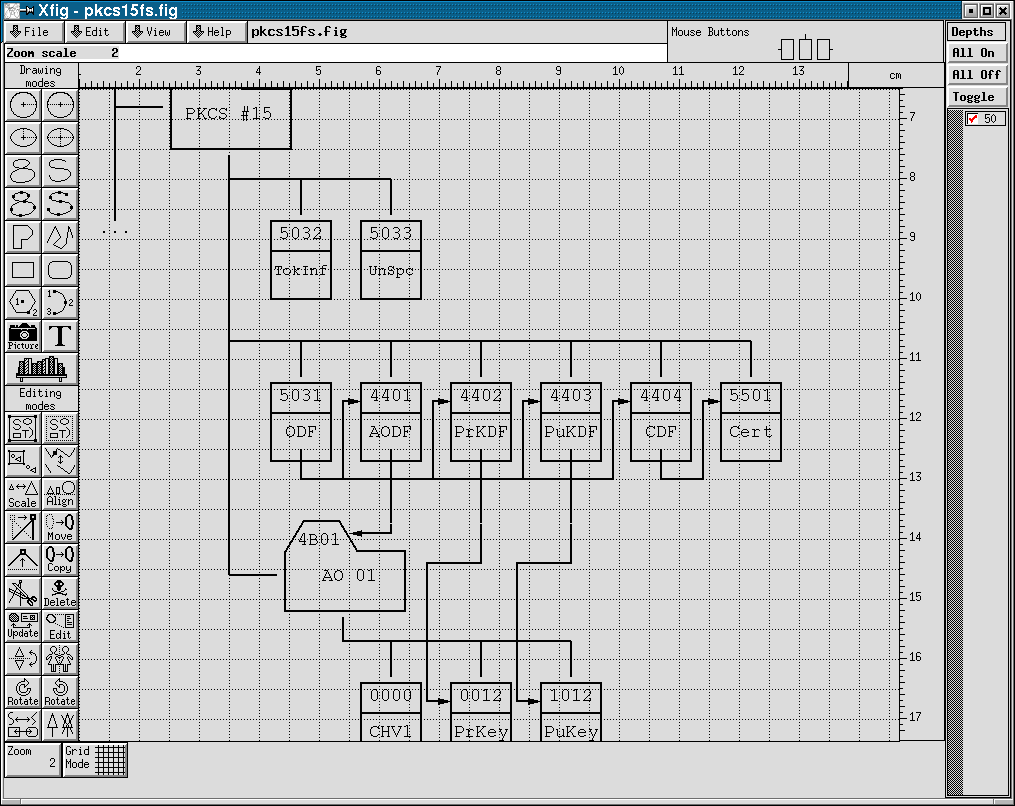
\includegraphics[angle=0,scale=.35]{img/xfig.png}
    \end{center}
    \caption{\em Xfig}
    \label{fig:xfig}
\end{figure}

\section{Przykład piąty}

Po utworzeniu pliku konfiguracyjnego można przystąpić do przygotowania
katalogów służących do przechowywania danych CA (zgodnie z~wcześniej
założonymi nazwami w~{\em openssl.cnf}). Tworzymy katalog {\em ca}, a~w nim
katalogi {\em certs}, {\em crl}, {\em private}, {\em newcerts} oraz pliki
{\em serial.txt} (z wpisem 01) i~{\em index.txt}. Plik {\em openssl.cnf} należy
umieścić na tym samym poziomie co katalog {\em ca}. Oczywiście możliwe jest
zupełnie inne zorganizowanie sposobu przechowywania danych w~CA, jednak
musi ono odpowiadać wcześniej przyjętym założeniom w pliku konfiguracyjnym.

Następnym krokiem przy tworzeniu CA jest wygenerowanie pary kluczy oraz
autocertyfikatu (w przypadku, gdy certyfikat dla centrum nie będzie
poświadczany przez inne centrum certyfikacji) dla centrum certyfikacji.

\begin{verbatim}
# generacja klucza prywatnego RSA o długości 4096 bitów
# do pliku cakey.pem (klucz w formie jawnej)
openssl genrsa -out ca/private/cakey.pem 4096 -config openssl.cnf

# utworzenie autocertyfikatu centrum (cacert.pem) o strukturze
# X.509 i formacie PEM dla klucza jawnego związanego z kluczem
# tajnym cakey.pem
openssl req -new -x509 -days 1825 -key ca/private/cakey.pem -out
    ca/cacert.pem -config openssl.cnf
\end{verbatim}

Po tych operacjach CA jest gotowe do pracy.

\section{Przykład szósty}

Oto przykładowy wydruk:
\begin{lstlisting}[language=Java,style=outcode,caption=Przykładowy wydruk]
import a.b.c;

// komentarz

/*
 * Komentarz...
 */
public class A
{
	int A;
	int B; // zmienna

	A()
	{
		A=1;
		/* to jest komentarz */
	}

	public void metodaA(int i)
	{
		for (int a=i; a<100; ++a)
		{
			short sw=(short)a;
			// ...
		}
	}
}
\end{lstlisting}

A oto wydruk wpleciony w tekst\dots
\begin{lstlisting}[language=C,style=incode]
/* ta funkcja oblicza a+b */
int sum(int a, int b)
{
	int suma=0;

	suma=a+b;

	return suma;
}
\end{lstlisting}
\dots i tekst za kodem.

% \lstinputlisting[language=Java,style=incode]{nazwa pliku}

% ex: set tabstop=4 shiftwidth=4 softtabstop=4 noexpandtab fileformat=unix filetype=tex spelllang=pl,en spell:

%%%% ROZDZIAŁ PIERWSZY %%%%%%%

\chapter{Wprowadzenie}
\section{Motywacja}
Z usług hotelowych korzystał prawdopodobnie każdy z nas. Nie każdy natomiast wie jak wygląda sytuacja po drugiej stronie. Hotelarz musi poradzić sobie z dużym wolumenem danych, które zmieniają się dość dynamicznie. Goście przyjeżdżają i wyjeżdżają, napływają kolejne rezerwacje, inne są odwoływane, pokoje muszą być czyste na czas, zamówione usługi przez gości muszą być wykonane na ich życzenie. Kontrola tych wszystkich informacji i synchronizacja pracy w czasie wymaga wsparcia ze strony systemu informatycznego.

\section{Cel pracy}
Celem pracy było stworzenie prototypu aplikacji zarządzającej obłożeniem hotelu. Założeniem pracy było wykorzystanie architektury trójwarstwowej przy budowie aplikacji. Kolejnym założeniem był wybór języka Java, który jest obiektowym językiem wysokiego poziomu. Wybrana architektura pozwoliła na zbudowanie prototypu aplikacji o niskim koszcie utrzymania oraz wysokim potencjale rozwoju.

\chapter{Analiza dziedziny} 
\label{analiza-dziedziny}
Niniejszy rozdział przedstawia wyniki analizy dziedziny hotelarstwa. Opracowanie zawiera ogólne omówienie hotelarstwa oraz organizacji hotelu oraz pojęcia potrzebne do zrozumienia oraz zaprojektowania systemu zarządzania obłożeniem. Rozdział kończy się porównaniem istniejących systemów.

\section{Źródła informacji}

Analiza dziedziny powstała na wskutek agregacji i uporządkowania informacji 
z kilku źródeł. Posłużyłem się literaturą branżową, ustawą i informacjami z 
internetu jak również uzyskałem informację przeprowadzając rozmowy z 
pracownikami hoteli na różnych stanowiskach. Miałem okazję rozmawiać z 
recepcjonistką oraz kierownikiem recepcji w dwóch różnych hotelach w 
Warszawie. Czytelnik znajdzie poniżej przefiltrowane, spójne wiadomości na
 temat branży hotelarskiej.


\section{Historia hotelarstwa} 

Ludzie zmieniali swoje miejsce pobytu od tysiącleci. Dlaczego? Powody były różne 
\mbox{i przez} tysiąclecia znacząco się nie zmieniły. Kiedyś wędrówki handlowe, \mbox{a 
dziś} wyjazdy biznesowe, religijne wyprawy w miejsca kultu lub podróże 
turystyczne do atrakcyjnych, bądź historycznych miejsc. Historia 
hotelarstwa ma bogatą przeszłość i sięga aż II tysiąclecia p.n.e gdzie na 
terenach Bliskiego Wschodu znaleziono pierwsze ślady budownictwa 
nastawionego na gościnę podróżnych. Najstarsze domy zajezdne odnotowano 
wzdłuż szlaków handlowych w miejscach obfitujących w wodę pitną. \mbox{W 
starożytnej} Grecji i Rzymie budowano zajazdy w miejscach kultu religijnego, 
bądź blisko miejsc odbywania się igrzysk. W czasach Średniowiecza gościny udzielano 
w klasztorach, początkowo nieodpłatnie, z czasem jednak gościna przyjęła 
formę rynkową. Edykt Karola Wielkiego nałożył na klasztory \mbox{i kościoły} 
obowiązek utrzymania hospicjów, gdzie podróżnym udzielano wyżywienia, 
kąpieli \mbox{i opieki} medycznej. Najgęstsza sieć hospicjów znajdowała się na 
terenie dzisiejszej Szwajcarii. Szwajcaria posiada najdłuższe tradycje 
hotelarskie \mbox{i jest} uważana \mbox{za wzór} hotelarstwa takiego jak znamy dzisiaj.


\section{Hotelarstwo i usługa hotelarska}

\subsection{Czym charakteryzuje się hotelarstwo?}

Hotelarstwo to forma działalności gospodarczej charakteryzująca się:
\begin{itemize} 
  \item szczególnym rodzajem gościnności - gościnność za odpłatnością,
  \item różnego rodzaju działalnością usługową. Główne z 
  nich to usługi bytowe takie jak zapewnienie noclegu oraz wyżywienia,
  \item określonym w czasie i z reguły krótkotrwałym pobytem gości,  
  \item zakresem usług świadczonych przez hotelarzy rozszerzanym o innego rodzaju działalność turystyczną i rozrywkową.
\end{itemize}

\subsection{Definicja usługi hotelarskiej}

Czym jest usługa hotelarska? Na to pytanie odpowiada treść \textit{Ustawy o usługach 
turystycznych} \cite{ust:tur}.

\begin{defn}{Usługa hotelarska:}

krótkotrwałe, ogólnie dostępne wynajmowanie domów, mieszkań, pokoi, miejsc 
noclegowych, a także miejsc na ustawienie namiotów lub przyczep 
samochodowych oraz świadczenie, w obrębie obiektu, usług z tym związanych.

\end{defn}

Usługi hotelarskie zaspokajają więcej potrzeb niż może to wynikać z 
definicji, a są to: wypoczynek, pożywienie, nocleg, higiena, rekreacja, 
rozrywka, zapewnienie bezpieczeństwa, opieka nad zdrowiem, zapewnienie 
wygody, dobrej atmosfery pobytu i inne drobne usługi.

Pewne usługi są regulowane prawnie, poprzez przepisy dotyczące wymagań 
rodzajowych i kategoryzacyjnych. Jednakże abstrahując od przepisów można 
stwierdzić, iż w interesie każdego hotelarza jest zapewnienie tak bogatej 
palety usług, jak to możliwe, aby wyróżniać się na rynku i przyciągać gości. 
Spełnienie minimum wymaganego prawnie nie jest szczególnie atrakcyjne z 
punktu widzenia gościa. Więcej o usługach dowiemy się w dalszej części pracy.

\section{Klasyfikacja i kategoryzacja obiektów hotelarskich}
Klasyfikacja określa podział obiektów na rodzaje. Rodzaje obiektów różnią 
się miedzy sobą zakresem działalności.

Definicje obiektów określa Rozporządzenie Ministra Gospodarki i Pracy z dnia 
19 sierpnia 2004 roku, oto część z nich:

\begin{itemize}
  \item hotele - obiekty posiadające co najmniej 10 pokoi, w tym większość 
  miejsc w pokojach jedno- i dwuosobowych, świadczące szeroki zakres usług 
  związanych z pobytem klientów;
  \item motele - obiekty położone przy drogach, dysponujące parkingiem, 
  posiadające \mbox{co najmniej} 10 pokoi, w tym większość miejsc w pokojach jedno- 
  i dwuosobowych;
  \item pensjonaty - obiekty posiadające co najmniej 7 pokoi, świadczące dla 
  swoich klientów całodzienne wyżywienie;
  \item kempingi - obiekty strzeżone, umożliwiające nocleg w namiotach i 
  przyczepach samochodowych, domkach turystycznych lub innych obiektach 
  stałych, oraz przyrządzanie posiłków i parkowanie samochodów.
\end{itemize}

Rozporządzenie definiuje także domy wycieczkowe, schroniska młodzieżowe, 
schroniska i pola biwakowe. Wiele obiektów nie zostało zdefiniowanych, m.in. 
ośrodki wczasowe, kwatery prywatne, internaty, domy studenckie.


\subsection{Podział według kategorii} 
Obiekty hotelarskie można podzielić według różnych kategorii\cite[15-16]{
KlasKatZakHot}:

\begin{enumerate}
  \item według lokalizacji:
    \begin{itemize}
      \item hotele miejskie
      \item obiekty wypoczynkowe, sportowe, kuracyjne
      \item motele - przy szlakach komunikacyjnych
    \end{itemize}
  \item według średniego pobytu gościa w obiekcie:
    \begin{itemize}
      \item hotele i pensjonaty stale lub prawie stale czynne
      \item zakłady rezydenckie (minimum 10-15 dni)
      \item hotele dla przejezdnych (2-3 dni)
    \end{itemize}
  \item według zakresu świadczonych usług:
    \begin{itemize}
      \item hotel pełny - pełny zakres usług
      \item hotel pensjonat - brak restauracji dla gości z zewnątrz, brak 
      napojów alkoholowych
      \item hotel garni - tylko wydawanie śniadań i prowadzenie bufetu
    \end{itemize}
  \item według okresu eksploatacji:
    \begin{itemize}
      \item stałe
      \item sezonowe
    \end{itemize}
  \item według siedziby obiektu:
    \begin{itemize}
      \item stałe
      \item ruchome - zakłady w okresie ferii, domki kempingowe, wagony 
      sypialne, samoloty
    \end{itemize}
  \item według dostępności:
    \begin{itemize}
      \item otwarte - ogólnodostępne
      \item półotwarte - domy wczasowe, domy zdrojowe
      \item zamknięte - tylko dla określonych grup ludności - domy 
      akademickie, sanatoria.
    \end{itemize}
\end{enumerate}

\subsection{Wymagania kategoryzacyjne}
Wymagania dla obiektów kategoryzowanych określa przywołane wyżej rozporządzenie. 
Ustalono w nim następujące kategorie bazy noclegowej:

\begin{itemize}
  \item dla hoteli, moteli i pensjonatów - pięć kategorii oznaczonych 
  gwiazdkami,
  \item dla kempingów - cztery kategorie oznaczone gwiazdkami,
  \item dla domów wycieczkowych i schronisk młodzieżowych - trzy kategorie 
  oznaczane cyframi rzymskimi.
\end{itemize}

Kategoryzacja niesie ze sobą wymagania. Każda kategoria ma ściśle określone 
kryteria, które obiekt musi spełniać. Kryteria te określają minimalny poziom 
świadczonych usług. Wprowadzają też porządek do słownictwa i umożliwiają 
standaryzację obiektów. Szczególną uwagę poświęcę pięcio-gwiazdkowej 
kategoryzacji.

\subsection{Pięć gwiazdek}
Prawdopodobnie wszyscy znają ten podział, a przynajmniej orientują się, że im 
więcej gwiazdek, tym wyższy standard. Różne turystyczne oferty mamią nas 
gwiazdkami. Warto wiedzieć, na co faktycznie możemy liczyć, ale czy na pewno 
nasze oczekiwania zostaną spełnione? 

Kategoryzacja istnieje w wielu krajach 
europejskich, ale jedna jest drugiej nierówna. Szczegółowość krajowych wymagań dla 
kategorii różni się. Nie wszędzie jest to także regulowane 
prawnie. W Niemczech nie ma kategoryzacji, \mbox{a kategorie} obiektów są stosowane 
w sposób umowny przez wydawców przewodników i biura podróży. Warto mieć to 
na uwadze przy planowaniu podróży.

\section{Podział usług hotelarskich}   
Podstawowymi usługami świadczonymi przez hotel są usługi noclegowe i 
gastronomiczne. Wszystkie inne usługi są im podporządkowane.

Wszystko, co wykracza poza usługi podstawowe, można podzielić w następujący 
sposób:
  \begin{itemize}
    \item usługi uzupełniające
    \item usługi fakultatywne
    \item usługi towarzyszące.
  \end{itemize}

\subsection{Usługi uzupełniające}
Usługi uzupełniające dopełniają podstawowe usługi i są z nimi bezpośrednio 
związane. Gość jest zmuszony z nich korzystać, w momencie gdy decyduje się na 
pobyt w hotelu. Przykładami usług uzupełniających są:

\begin{itemize}
  \item budzenie
  \item szatnia
  \item depozyt
  \item informacja turystyczna.
\end{itemize}

Usługi uzupełniające są zazwyczaj bezpłatne, ponieważ są wliczone w cenę 
usług podstawowych.

\subsection{Usługi fakultatywne}
Kolejny rodzaj usług to usługi fakultatywne. Te usługi są już mniej 
powiązane z usługami podstawowymi. Usługi fakultatywne uatrakcyjniają pobyt 
gościom. Przykłady takich usług to:

\begin{itemize}
  \item basen
  \item sauna
  \item tenis
  \item rozrywka.
\end{itemize}

Podczas pobytu korzystanie z usług fakultatywnych jest opcjonalne, ale zazwyczaj trzeba być 
gościem hotelu, żeby móc z nich skorzystać. To, czy te usługi są płatne czy 
nie, zależy od hotelu.  Jeśli są bezpłatne, stanowią zachętę dla gości (mimo 
tego, że mogą być wliczone w cenę).

\subsection{Usługi towarzyszące}
Usługi towarzyszące są całkowicie ortogonalne w stosunku do usług 
podstawowych. Oznacza to, że nie trzeba być hotelowym gościem, aby móc z 
nich skorzystać. Tak samo jak usługi fakultatywne, usługi towarzyszące są 
opcjonalne. Usługi towarzyszące to odrębny rodzaj działalności z lokalizacją 
przy hotelu. Przykładami usług towarzyszących są:

\begin{itemize}
  \item kiosk
  \item kwiaciarnia
  \item kasyno
  \item usługi handlowe.
\end{itemize}

\subsection{Usługi obce}
Te usługi, które są świadczone bezpośrednio przez obsługę hotelową, nazywa 
się usługami własnymi. Są jednak pewne usługi dodatkowe, których hotel nie 
może świadczyć. Sprzedawanie usług dodatkowych, 
korzystając z zewnętrznych firm, pozwala hotelowi zwiększyć swoją \mbox{atrakcyjność.} Przykładem usług obcych mogą być wszelakie usługi turystyczne, 
które organizuje zewnętrzne biuro turystyczne.

Usługi obce to także dostarczanie energii elektrycznej, wody i innych mediów.
 Tutaj hotel jest zdany na innych operatorów, ponieważ samemu nie może wszystkiego 
wytworzyć.

\subsection{Wymagania kategoryzacyjne a usługi}
Część usług dodatkowych może być wymuszona poprzez wymagania kategoryzacyjne.
 Te usługi są \emph{obowiązkowe}. Reszta usług dodatkowych, świadczonych 
 przez hotel dla wygody gości i podniesienia prestiżu 
 hotelu, to usługi \emph{dobrowolne}.

\section{Istotne definicje}
\subsection{Definicja noclegu}

\begin{defn}{Nocleg}

Usługa noclegowa dla jednej osoby w wymiarze jednej doby hotelowej, \mbox{tzw. 
osobodzień.} Nocleg jest jednostką miary usługi noclegowej.

\end{defn} 

Nocleg wykorzystywany jest w miernikach usług hotelarskich:
\begin{itemize}
  \item nominalna liczba noclegów - liczba miejsc, które można wynająć w 
  danym okresie.
  \item wskaźnik frekwencji - stopień wykorzystania miejsc w procentach.
\end{itemize}

\subsubsection{Wskaźnik RevPAR}
Podstawowym wskaźnikiem jest wskaźnik RevPAR\footnote{ang. Revenue per 
available room.}. RevPAR określa zrealizowane, 
dzienne obroty każdego wybudowanego pokoju. Liczony jest na podstawie
 ilorazu dochodów z pokoi do liczby wszystkich dostępnych pokoi w hotelu. RevPAR uwzględnia tylko 
 dochód z wynajmu pokoi. Nie brane są pod uwagę inne źródła dochodu, czyli np. te ze sprzedaży usług.

\begin{equation}
RevPAR = \frac{Rooms Revenue}{Rooms Available}
\end{equation}

Może być także oszacowany w następujący sposób:

\begin{equation}
RevPAR \approxeq Freq \cdot ADR
\end{equation}

\begin{description}
  \item[Freq] wskaźnik frekwencji. Procent okupowanych pokoi.
  \item[ADR]\footnote{ang. {\em Average Daily Rate}. } średnia stawka (netto) 
  za pokój bez śniadania. ADR liczone jest jako iloraz przychodów netto ze 
  sprzedaży pokoi i liczby sprzedanych pokoi.

\end{description}

\subsection{Definicja doby hotelowej}
Doba hotelowa różni się od zwykłej doby.

\begin{defn}{Doba hotelowa} - trwa do godziny określonej jako godzina 
zakończenia doby 
hotelowej. Godzina zakończenia doby hotelowej jest ustalana przez hotel.
 Długość doby hotelowej dla gościa może być większa lub mniejsza 
od normalnej doby. Doba hotelowa została wprowadzona ze względu na 
organizację pracy hotelu, m.in. sprzątania pokoi.

\end{defn}

Załóżmy, że godzina zakończenia doby hotelowej to 12.00. Jeśli gość 
przyjechał o godzinie 10.00 to będzie mógł korzystać z pokoju do godziny 12.00 
następnego dnia, a więc więcej niż 24 godziny. Przyjeżdżając po godzinie 12.00, 
będzie mógł korzystać z pokoju krócej. W obu przypadkach gość zapłacił tyle 
samo za pojedynczą dobę hotelową.


\subsection{Klient}

Klient bądź gość również został zdefiniowany w ustawie\cite{ust:tur}:

\begin{defn}{Klient}
- osoba, która zamierza zawrzeć lub zawarła umowę \mbox{o świadczenie} usług 
turystycznych na swoją rzecz lub na rzecz innej osoby, \mbox{a zawarcie} tej umowy 
nie stanowi przedmiotu jej działalności gospodarczej, jak \mbox{i osobę}, na rzecz 
której umowa została zawarta, \mbox{a także} osobę, której przekazano prawo \mbox{do 
korzystania} z usług turystycznych objętych uprzednio zawartą umową.

\end{defn}

Definicja bazująca na ustawie jest dość skomplikowana, więc można spróbować 
prościej:

\begin{defn}{Klient}
- osoba, korzystająca z usług hotelarskich, w szczególności usługi noclegowej.

\end{defn}

Klient oraz gość nie znaczą dokładnie tego samego, ponieważ, jak wiemy, 
hotel świadczy usługi towarzyszące, których świadczeniobiorca nie musi być 
gościem hotelowym. Jednak, nie wdając się w szczegóły, 
będziemy używać tych nazw wymiennie. Więcej o klientach dowiemy się w rozdziale
\ref{rodzaje-klientow}.

\subsection{Agent}
Agent biura turystycznego pełni rolę pośrednika. Zazwyczaj biuro turystyczne 
wykupuje pewny pakiet noclegów w hotelu. Kupując hurtowo, otrzymuje niższe 
ceny niż zwykli klienci, a zatem może pozwolić sobie na ciekawszą ofertę. 
\mbox{Oto definicja} agenta\cite{ust:tur}:

\begin{defn}{Agent turystyczny}
- przedsiębiorca, którego działalność polega \mbox{na stałym} pośredniczeniu w 
zawieraniu umów o świadczenie usług turystycznych \mbox{na rzecz} organizatorów 
turystyki posiadających zezwolenia w kraju lub \mbox{na rzecz} innych usługodawców 
posiadających siedzibę w kraju.
\end{defn}

\section{Organizacja w zakładzie hotelarskim}
Przyjrzymy się teraz organizacji w zakładzie hotelarskim. Organizacja w 
zakładzie hotelarskim zależy od typu tego zakładu.

Inaczej będzie wyglądać organizacja w małym pensjonacie, prowadzonym przez 
kilka osób (np. rodzinę), a inaczej organizacja dużego 
luksusowego hotelu nastawionego na klientów biznesowych. 

W pierwszym przypadku członkowie rodziny i kilku pracowników mają szeroki 
zakres obowiązków i oczekiwane jest wykonywanie działań, które aktualnie są 
potrzebne. Struktura organizacja będzie dość prosta i płaska.

W przypadku znacznie większego hotelu, który zatrudnia znaczącą liczbę 
pracowników i obsługuje kilkuset gości, wymagana będzie bardziej rozbudowana 
struktura organizacyjna. Przyjrzymy się podobnemu przypadkowi z bliska i 
poznamy, jak może wyglądać taka struktura. 

Zanim jednak do tego przejdziemy zapoznajmy się z definicją struktury.

\subsection{Definicja struktury}
Definicja na podstawie \cite{bk:def-struktury}:
\begin{defn}{Struktura} 
to instrument zarządzania organizacją. To uporządkowanie pozycji w 
organizacji według zasad podziału pracy, co wiąże się z określeniem 
specjalistycznych zadań, które muszą być wykonane, aby organizacja mogła 
funkcjonować i osiągać założone cele. To zgrupowanie ról organizacyjnych w 
większe całości, podsystemy: sekcje, wydziały, zakłady, piony - gdzie 
następuje obarczenie odpowiedzialnością za sprawną realizację zagregowanych 
zadań poszczególnych komórek organizacyjnych, a zwłaszcza kierowników tych 
podsystemów. To w końcu podział władzy i informacji w ramach organizacji, a 
więc uporządkowanie pionowego podziału pracy w ramach szczebli struktury 
(poziomów jej hierarchii).
\end{defn}

\subsection{Struktura organizacyjna w średniej wielkości hotelu}
Pod lupę weźmiemy średniej wielkości hotel. Na tyle duży, że wymaga 
wprowadzenia struktury organizacyjnej, ale na tyle nieskomplikowanej, że można 
będzie \mbox{ją przedstawić} w prosty sposób.

\subsubsection{Przykład struktury organizacyjnej hotelu}
Przykładową strukturę organizacyjną przedstawia poniższy rysunek 
(\ref{fig:struktura-hotelu}).

\begin{figure}[H]
  \begin{center}
  \fbox{
    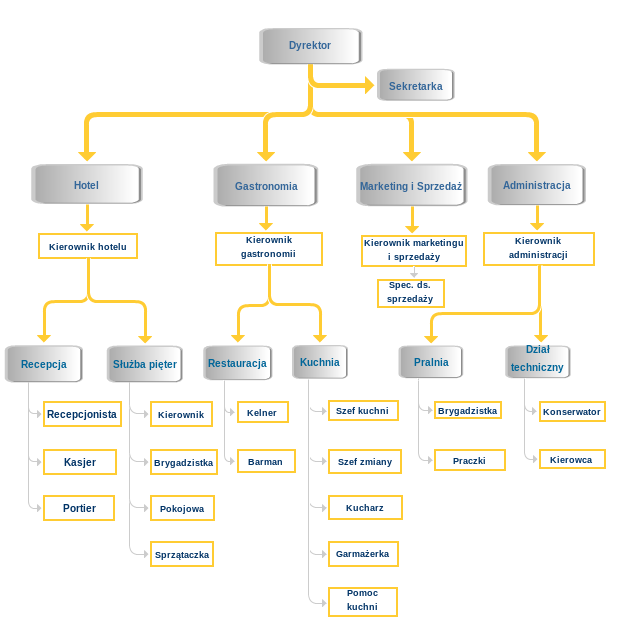
\includegraphics[width=\textwidth]{../img/struktura.png}
  }
  \end{center}
  \caption{Przykładowa struktura hotelu}
  \label{fig:struktura-hotelu}
\end{figure}

\subsubsection{Charakterystyka przykładowej struktury}
Na szczycie struktury znajduje się dyrektor, ale bardziej interesujący jest dalszy 
podział jego organizacji. Struktura zawiera w sobie dwie struktury:
\begin{itemize}
  \item strukturę produkcyjną - zaliczają się do niej wszystkie działy i 
  komórki, które \mbox{w sposób} bezpośredni związane są z \emph{produkcją}
  jednostki mieszkalnej gotowej \mbox{do sprzedaży}, sali konferencyjnej do 
  wynajmu, posiłku do wydania;
  \item strukturę administracyjną - do której należą wszystkie działy, które
   nie są \mbox{w strukturze} produkcyjnej. Na rysunku pominąłem dział księgowy, 
   który jak zalicza się do struktury administracyjnej.
\end{itemize}

Struktura podzielona jest na 4 działy:
\begin{itemize}
  \item Dział Hotelarski - omówiony poniżej
  \item Dział Gastronomiczny - odpowiada za przygotowanie posiłków i napoi 
  do sprzedaży. Zapewnia gościom hotelowym wyżywienie w zakresie co najmniej 
  śniadania,
  \item Dział Marketingu i Sprzedaży - realizuje działania, w efekcie 
  których klient wybiera ten, a nie inny hotel,
  \item Dział Administracyjny - finanse, remonty, usługi wewnętrzne, 
  koordynacja działania przedsiębiorstwa
\end{itemize}

Działania tych działów muszą być koordynowane, tak aby każdy z nich 
efektywnie uczestniczył w zaspokajaniu potrzeb gości. Za każdy dział 
odpowiedzialny jest kierownik, który odpowiada przed dyrektorem. Dyrektor
 nadzoruje i koordynuje działania kierowników.

\subsection{Dział Hotelarski}
W naszym przykładzie dział hotelarski składa się z:
\begin{itemize}
  \item węzła recepcyjnego - scharakteryzowanego poniżej,
  \item służby pięter - odpowiedzialnej za utrzymanie czystości w hotelu, 
  przygotowanie jednostek mieszkalnych do sprzedaży oraz ciągów 
  komunikacyjnych do użytkowania.
\end{itemize}

Wymienione wyżej działy to tylko przykład, ponieważ struktura 
organizacyjna może być o wiele bardziej skomplikowana.

Przyjrzyjmy się bliżej węzłowi recepcyjnemu.

\subsection{Węzeł recepcyjny}
Recepcja pełni ważną rolę w strukturze organizacyjnej. Od strony gościa hotelu, 
można powiedzieć, że nawet najważniejszą. 
Recepcja obsługuje klienta od momentu przyjęcia rezerwacji, w ciągu pobytu, 
aż do zakończenia pobytu i opuszczenia hotelu przez gościa. Recepcja spełnia 
także funkcje marketingowe 
oraz sprzedażowe. Posiada także funkcje zakwaterowania i obsługi gościa 
podczas pobytu. Jako, że sam proces zakwaterowania jest bardzo krótki i trwa 
kilka, kilkanaście minut, można powiedzieć, że najważniejszą i główną funkcją 
węzła recepcyjnego jest obsługa gościa w trakcie jego pobytu.

Recepcja pełni także funkcję sprzedażową, ponieważ klient, 
który przyjdzie wprost z ulicy, chcąc wynająć pokój, skieruje się do recepcji. 
Jest to zatem  bardzo ważna komórka i jedna z pierwszych, z którą spotyka 
się gość podczas swojego pobytu. Oprócz tego pracownicy recepcji mogą 
oferować płatne usługi, co także tłumaczy funkcję sprzedażową.

Potocznie mówi się, że pierwsze wrażenie jest najważniejsze. Recepcja jest 
dobrym tego przykładem. To od pracowników recepcji zależy, jakie hotel zrobi 
pierwsze wrażenie na kliencie. Od jakości obsługi podczas pobytu zależeć 
będzie, czy to pierwsze wrażenie zostanie utrzymane, a tym samym 
czy klient opuści hotel szczęśliwy i będzie chciał wkrótce wrócić czy też
 nie.


\subsubsection{Pracownicy recepcji}
W recepcji funkcjonują \cite{OrgaDzialHot}:

\begin{itemize}
  \item kierownik recepcji - odpowiada za sprawne 
  funkcjonowanie recepcji,
  \item recepcjonista dysponent - do jego zadań należy m.in przydzielanie 
  pokoi gościom na dany dzień na podstawie rezerwacji i pokoi zwalnianych,
  \item recepcjonista klucznik - m.in. zarządza kluczami, rozdziela 
  korespondencję, przyjmuje zlecenia, np. na budzenie,
  \item recepcjonista ds. rezerwacji,
  \item recepcjonista kasjer - przyjmuje gotówkę, wymienia walutę,
  \item recepcjonista informator (consierge) - zajmuje się sprawami gości 
  hotelowych, np. zakupem biletów na koncert.
\end{itemize}

\subsubsection{Obowiązki recepcji} 
Recepcja odpowiada za \cite{OrgaDzialHot}:

\begin{itemize}
  \item przyjmowanie i realizację zleceń na rezerwację miejsc noclegowych,
  \item przyjmowanie gości,
  \item wystawianie kart pobytu,
  \item prowadzenie ewidencji gości zgodnie z obowiązującymi zasadami,
  \item wydawanie kluczy do pokoi, prowadzenie właściwej ich ewidencji oraz 
  ich zabezpieczenie,
  \item organizowanie pomocy przy przyjazdach i wyjazdach, ze szczególnym 
  uwzględnieniem opieki nad bagażem gości,
  \item udzielanie informacji gościom oraz realizowanie na ich rzecz 
  dodatkowych usług,
  \item sporządzanie codziennych grafików wykorzystania pokoi,
  \item sprawne działanie w przypadkach losowych,
  \item przyjmowanie reklamacji gości,
  \item opieka nad korespondencją,
  \item przyjmowanie mienia gości do depozytu.
\end{itemize}

\subsubsection{Zespoły recepcji}
W recepcji można wyróżnić następujące zespoły\cite{hotel2:part1}:
\begin{enumerate}
  \item hall recepcyjny - część ogólnodostępna,
  \item lada recepcyjna,
  \item cześć wewnętrzna, usytuowana z reguły za ladą,
  \item służba parterowa.
\end{enumerate}

\section{Klasyfikacja hoteli raz jeszcze}
W pierwszym spojrzeniu na hotel, jego organizację, świadczone usługi i 
hotelowych gości, można go zaklasyfikować do jednej z dwóch grup:

\begin{itemize}
  \item Hotel Turystyczny
  \item Hotel Biznesowy.
\end{itemize}

Różnice będą widoczne w usługach, wystroju wewnętrznym i zewnętrznym, 
lokalizacji i nastawieniu na klienta.

Różnica będzie także w rocznym obłożeniu hoteli. Hotele turystyczne będą 
cieszyć się wysokim obłożeniem w sezonie turystycznym i zazwyczaj 
mniejszym poza tym okresem. Porównując obłożenia zauważymy, że hotele biznesowe 
charakteryzują się bardziej równomiernym obłożeniem w ciągu roku. 
Wyjątek stanowi okres konferencyjny, który rozpoczyna się na przełomie 
marca i kwietnia. Wówczas hotele biznesowe odnotowują zwiększone obłożenie,
 zwłaszcza te z dużą bazą konferencyjną.

Ciekawostką jest to, że pobyt w hotelu turystycznym będzie droższy w ciągu 
weekendu. Odwrotna sytuacja występuje w klasie biznesowej.

\section{Pomieszczenia hotelowe}
Hotel posiada liczne pomieszczenia. Tylko część z nich jest ogólnodostępna 
dla gości. Są to np. jednostki mieszkalne. Niektóre z pomieszczeń dostępne są całodobowo, np. recepcja, a niektóre tylko w określonych godzinach, np. sale restauracyjne.

Niektóre pomieszczenia to m.in.:
\begin{itemize}
\item hol,
\item recepcja,
\item jednostki mieszkalne,
\item sala restauracyjna,
\item sale konferencyjne,
\item magazyny,
\item zaplecze techniczne,
\item biura,
\item ciągi komunikacyjne,
\item winda,
\item korytarze.
\end{itemize}

Przyjrzymy się bliżej jednemu z pomieszczeń.

\section{Pokoje}
Najbardziej znanymi pomieszczeniami hotelowymi są jednostki mieszkalne, czyli 
potocznie mówiąc pokoje hotelowe. Kontynuując opis naszego przykładowego 
hotelu, będziemy mogli przedstawić rodzaje pokoi w hotelu.

\subsection{Rodzaje pokoi}
Poniżej zostały wymienione rodzaje pokoi wraz z ich angielskimi nazwami.

Rodzaje pokoi hotelowych:
\begin{itemize}
  \item pokój jednoosobowy (ang. single room)
  \item pokój dwuosobowy (ang. double room)
  \item pokój trzyosobowy (ang. triple room)
  \item pokój z dostawką (ang. room with additional bed)
  \item pokój przystosowany do obsługi gości niepełnosprawnych (ang. room for 
  handicapped)
\end{itemize}

\section{Karta pobytu}
Karta pobytu to dokument, który gość otrzymuje po pomyślnym zakwaterowaniu. 
Karta pobytu zawiera najważniejsze informacje o dobie hotelowej, ciszy 
nocnej, warunkach bezpieczeństwa oraz usługach dodatkowych w hotelu i 
gastronomii. Może także zawierać szkic miasta z zaznaczonym hotelem.

Karta pobytu spełnia dwie funkcje:
\begin{itemize}
  \item{informacyjną}, przypomina gościom o podstawowych informacjach,
  \item{zabezpieczającą}, służy do identyfikacji gościa pobierającego klucz 
  lub podpisującego rachunek.
\end{itemize}

\section{Rezerwacja}
Rezerwacja jest bardzo ważnym dokumentem w hotelarstwie. Jeszcze niedawno 
proces przyjmowania rezerwacji był jedną z częściej wykonywanych czynności 
przez recepcjonistę. Tam gdzie nie ma automatyzacji i możliwości dokonania 
rezerwacji przez internet, nadal tak jest. Tam gdzie jest to proces manualny, 
tam też istnieje możliwość pomyłki. Prawidłowe dokonanie rezerwacji jest 
sprawą kluczową zarówno dla gościa jak i dla hotelu. Rezerwacja może bowiem 
stanowić źródło wielu dodatkowych informacji przydatnych przy organizacji 
usług hotelarskich i działań marketingowych.

W następnych podrozdziałach przyjrzymy się bliżej rezerwacji, gdyż jest to 
kluczowy element w działalności hotelu. Zapoznamy się, w jaki sposób można jej dokonać, jakie są 
typy rezerwacji, jakie informacje zawiera i dowiemy się o wielu innych 
zagadnieniach związanych z rezerwacją.

\subsection{Co oznacza rezerwacja?}
Rezerwacja, która jest niepotwierdzona od strony prawnej, niewiele znaczy. 
Przyjęcie i potwierdzenie rezerwacji jest natomiast formą zawarcia umowy 
między gościem a hotelem do realizacji podstawowej usługi hotelarskiej, 
czyli gościnności za odpłatnością. Aby zatem przyjąć rezerwację, trzeba 
wiedzieć o obłożeniu hotelu, planowanych imprezach, planowanych remontach, 
tak aby móc zrealizować usługę w określonym terminie. Rezerwacja w ogólności 
jest dokonywana na typ pokoju, a nie konkretny pokój, aczkolwiek może być 
inaczej. Wynika z tego, że trzeba wiedzieć, jakie typy będą dostępne w 
określonym terminie.

\subsection{Sposoby przeprowadzania rezerwacji}
Jest kilka sposobów dokonania rezerwacji. Oto one:
\begin{itemize}
  \item dokonanie rezerwacji bezpośrednio w hotelu,
  \item dokonanie rezerwacji za pomocą faksu,
  \item dokonanie rezerwacji za pomocą internetu,
  \begin{itemize}
     \item bezpośrednio on line - uzupełniając formularz na 
     stronie hotelu
     \item pośrednio poprzez system klasy CRS \footnote{przykładowo 
     www.booking.com/index.pl.html} (\ref{system-crs})
  \end{itemize}
  \item dokonanie rezerwacji telefonicznie - podając dane 
  pracownikowi recepcji. Przez całą procedurę przeprowadzi nas pracownik w 
  recepcji\footnote{W sieci hoteli Marriott wszystkie dane powtarzane są 
  dwa razy, w celu sprawdzenia ich poprawności przez obie strony.},
  \item dokonanie rezerwacji poprzez biuro usług pośredniczących - które  
  może korzystać z wcześniej wymienionych sposobów lub poprzez system klasy 
  CRS (\ref{system-crs}). Istnieje jeszcze jedna możliwość, którą poznamy przy 
  okazji rezerwacji grupowych (\ref{rezerwacja-grupowa}).
\end{itemize}

\subsection{Rodzaje rezerwacji}
W celu zabezpieczenia hotelu przed stratami z tytułu anulowanych rezerwacji, 
\mbox{a tym} samym niewykorzystanych pokoi wprowadzono trzy rodzaje rezerwacji:

\begin{itemize}
  \item wstępną,
  \item gwarantowaną,
  \item niegwarantowaną.
\end{itemize}

To, czy wszystkie rodzaje rezerwacji są dostępne, zależy od hotelu. 

\subsubsection{Rezerwacja wstępna}
Dokonujemy rezerwacji i otrzymujemy termin, do którego musimy potwierdzić 
rezerwację. W przypadku braku potwierdzenia, rezerwacja zostaje anulowana. 
Żadna ze stron nie ponosi konsekwencji.

Jaki to będzie termin, zależeć będzie od hotelu. W przypadkach, gdzie 
głównie używana jest rezerwacja gwarantowana, może być tak, że terminem 
będzie godzina popołudniowa tego samego dnia, w którym dokonujemy rezerwacji.
 Zatem ma to sens, jeśli już jesteśmy w drodze do hotelu i chcemy zrobić 
 rezerwację bez podawania numeru karty kredytowej.

\subsubsection{Rezerwacja gwarantowana}
Jest to typowy rodzaj rezerwacji. Aby dokonać rezerwacji potrzebna jest 
pewna forma gwarancji, a dokładnie pewne zabezpieczenie finansowe. Jest gość{to 
najbezpieczniejszy} rodzaj rezerwacji dla hotelu.

Forma zabezpieczenia może być różna. Może to być przedpłata w określonym 
terminie. Może to być także obciążenie karty kredytowej. Karta kredytowa gość{to 
najczęściej} spotykany sposób płatności w przypadku dużych sieci hotelarskich. gość{W naszym} 
rodzimym przypadku spotkać się można z przedpłatą bankową.

Rezerwacja gwarantowana to sposób obrony hotelu przed stratami finansowymi. 
Jeśli gość zrezygnuje z rezerwacji, to w zależności od terminu straci 
całe zabezpieczenie lub jego część. Szczegóły zależą od zakładu hotelarskiego, 
ale zazwyczaj trzeba liczyć się z pewną karą.

Jeśli gość nie pojawi się planowanego dnia przyjazdu, to rezerwacja zostaje 
utrzymywana do dnia następnego, a gość zostaje obciążony kosztami pokoju za 
jedną noc, nie wliczając śniadania. Dalsza procedura zależy od hotelu, ale 
prawdopodobnie pracownik skontaktuje się z gościem, aby wyjaśnić zaistniałą 
sytuację.

Warto dodać, że metoda dokonania gwarancji nie ma związku z metodą płatności 
za pobyt.

\subsubsection{Rezerwacja niegwarantowana}
W odróżnieniu od rezerwacji gwarantowanej, dla tego typu rezerwacji nie ma 
konieczności zabezpieczenia w postaci depozytu. W przypadku niewykorzystania rezerwacji w określonym terminie umowa przestaje obowiązywać, 
a jej rozwiązanie nie pociąga ze sobą żadnych skutków finansowych. Całe 
ryzyko ponosi zatem hotel. Łatwo sobie wyobrazić szkodliwe działania konkurencji, 
które mogą wykorzystać ten sposób rezerwacji.

\subsection{Pojedyncza i grupowa rezerwacja}
Kolejnym podziałem rezerwacji jest podział na rezerwację indywidualną oraz 
grupową. 

\subsubsection{Rezerwacja indywidualna}
Rezerwacja indywidualna to rezerwacja dla klienta indywidualnego, czyli taka, 
jaką sami możemy zamówić w hotelu. Nie oznacza to jednak, że pobyt musimy 
spędzić samemu. Oznacza to, że rezerwacji dokonuje osoba prywatna. Dla tego typu rezerwacji ceny za pokój będą najwyższe.
Rezerwacja indywidualna może dotyczyć więcej niż jednego pokoju.

Zamiast samemu dokonywać rezerwacji możemy posłużyć się biurem pośrednictwa 
rezerwacji. Są to m.in biura turystyczne, biura linii lotniczych. Koszt rezerwacji dokonanej przez biuro pośrednictwa może być mniejszy. Powody tej zniżki poznamy w rozdziale omawiającym biuro turystyczne (\ref{biuro-turystyczne}).

\subsubsection{Rezerwacja grupowa}
\label{rezerwacja-grupowa}
Rezerwacja grupowa to rezerwacja dla klienta grupowego. Rezerwacji grupowych 
dokonuje wiele różnych instytucji. Są to m.in biura turystyczne, korporacje, 
stowarzyszenia, agencje podróży. Za wszystkie formalności związane z 
dokonaniem rezerwacji odpowiedzialny będzie pośrednik wynajęty przez grupę, 
bądź organizatora pobytu dla grupy. Grupa oznacza wiele osób - rezerwacja 
grupowa dotyczyć będzie zatem wielu pokoi. 

Opłata za rezerwację grupową zależeć będzie od sposobu jej organizacji. \mbox{W 
ogólnym} przypadku pobyt opłacony będzie poprzez organizatora grupy. 
Natomiast to czy dodatkowe usługi\footnote{usługi towarzyszące i fakultatywne}
 również będą wliczone w cenę, zależy od konkretnego przypadku. Istnieją trzy 
 możliwości:

\begin{itemize}
   \item organizator płaci za dodatkowe usługi,
   \item organizator nie płaci za dodatkowe usługi. Każdy członek grupy 
   płaci za korzystanie z usług,
   \item organizator płaci za dodatkowe usługi do pewnej kwoty. Nadwyżkę 
   opłaca członek grupy.
\end{itemize}

Ceny za pobyt będą atrakcyjniejsze w przypadku rezerwacji grupowych.

\subsubsection{Biuro turystyczne}
\label{biuro-turystyczne}
Biuro turystyczne jest jednym z podmiotów, które dokonują rezerwacji 
grupowych. Biura turystyczne posiadają także oferty dla klientów 
indywidualnych, \mbox{w których} koszta pobytu są niższe. Dlaczego tak jest?

Powody mogą być co najmniej dwa. Pierwsza możliwość jest taka, że biuro 
podróży nawiązuje z hotelem umowę, w której rezerwuje określoną liczbę 
pokoi wraz z określonymi usługami przy ustalonych warunkach cenowych - 
które będą korzystniejsze niż dla klienta indywidualnego. Najważniejszym dla 
biura jest termin, do którego musi powiadomić hotel \mbox{o faktycznym} 
wykorzystaniu miejsc. Jeśli \mbox{w wyznaczonym} terminie powiadomi hotel \mbox{i 
zmniejszy} liczbę pokoi to obciążone zostanie tylko za wykorzystaną liczbę, \mbox{a 
reszta} pokoi wróci do wolnej puli. Przy takiej umowie hotel zobowiązuje się, 
że określona liczba pokoi będzie dostępna i że nie będą one przedmiotem 
podobnej umowy z innym biurem turystycznym bądź inną instytucją.

Druga możliwość to tzw. \emph{allotment}. Biuro podróży wykupuje określoną 
liczbę miejsc za bardzo atrakcyjną cenę. Umowa ta również określa, w jakim 
terminie biuro ma prawo zrezygnować z całości lub części zamówionych pokoi 
bez ponoszenia kosztów. Hotel nie może zawierać na te miejsca innych umów.

Tymi sposobami biuro podróży może pozwolić sobie zaoferować niższe ceny. 
Jeśli skorzystamy z oferty otrzymamy voucher.

\begin{defn}{Voucher} 
to dokument indywidualny podobny do rezerwacji, który uprawnia beneficjenta 
do skorzystania z usługi.
\end{defn}

\subsection{Informacje na rezerwacji}
\label{chap1:info-na-rezerwacji}
Przy dokonywaniu rezerwacji możemy być pytani o wiele różnych informacji. 
Istnieje w miarę standardowa porcja informacji, którą zawsze trzeba podać. 
To, ile szczegółowych informacji będziemy mogli podać, zależeć będzie od 
\mbox{hotelu.} Bardzo szczegółową informacją są np. preferencje dotyczące 
rodzaju poduszki, bądź umiejscowienia pokoju blisko windy.

Podstawowe informacje, które podajemy przy dokonaniu rezerwacji to:

\begin{itemize}
  \item data przyjazdu,
  \item data wyjazdu,
  \item rodzaj pokoju,
  \item dane rezerwującego (klienta)
  \begin{itemize}
    \item tytuł,
    \item imię,
    \item nazwisko, 
    \item adres, 
    \item dane kontaktowe
  \end{itemize} 
  \item dane, dla kogo jest rezerwacja
  \begin{itemize}
    \item tytuł,
    \item imię
    \item nazwisko
    \item osoby dodatkowe
  \end{itemize}
  \item metodę płatności.
\end{itemize}

Niektóre z dodatkowych informacji, o które pytać będą hotele o wysokim 
standardzie:

\begin{itemize}
  \item czy pokój dla palących czy niepalących,
  \item umiejscowienie pokoju,
  \begin{itemize}
    \item niskie piętro,
    \item wysokie piętro,
    \item blisko windy,
  \end{itemize}
  \item widok,
  \item rodzaj poduszki,
  \item ile osób dorosłych,
  \item ile dzieci,
  \item informacje dodatkowe dla recepcji - specjalne życzenia bądź uwagi,
  \item preferencje żywieniowe.
\end{itemize}


\subsubsection{Potwierdzenie rezerwacji}
Potwierdzenie rezerwacji jest jej dokonaniem i tym samym jest 
zawarciem umowy między gościem a hotelem. Potwierdzenie rezerwacji może 
być przekazane drogą elektroniczną bądź tradycyjną. Potwierdzenie rezerwacji 
pozwala na sprawdzenie poprawności danych. Potwierdzenie rezerwacji stwarza 
możliwość reklamy innych usług zakładu hotelarskiego. 

Sam dokument z potwierdzeniem zawiera:
\begin{itemize}
  \item numer rezerwacji,
  \item datę zgłoszenia rezerwacji,
  \item adres hotelu,
  \item informacje podane przy dokonaniu rezerwacji,
  \item podsumowanie kosztów za pokój.
\end{itemize}

Może zawierać także numer rachunku bankowego, na który trzeba wpłacić 
zaliczkę wraz z terminem wpłaty.

\subsection{Odwoływanie rezerwacji}
Polityka odwołania rezerwacji określona jest podczas dokonywania 
rezerwacji. Zazwyczaj odwołanie rezerwacji jest możliwe i nie wiąże się z karami finansowymi, 
jeśli rezerwacja zostanie odwołana przed określonym terminem. 

Zazwyczaj, aby odwołać, rezerwację należy się skontaktować telefonicznie z 
hotelem. Jeśli nie pojawimy się w hotelu w dni przyjazdu, to typowym mechanizmem jest 
to, że nasza rezerwacja oznaczona będzie jako tzw. \emph{No show}. 

\begin{defn}{\emph{No show}}
- oznacza nie pojawienie się gościa w hotelu niepoprzedzone anulowaniem rezerwacji. 
Wiąże się z poniesieniem przez gościa ustalonych kosztów w zależności od 
rodzaju rezerwacji.
\end{defn}

Dalsza procedura to kontakt z rezerwującym następnego dnia, wyjaśnienie 
sytuacji, a w ostateczności obarczenie karą\footnote{np. wartość zabezpieczenia 
+ koszt jednej nocy}. Warto pamiętać o tym, że karanie klientów nie przynosi 
długoterminowych zysków, dlatego wspólny dialog z klientem i porozumienie 
jest pierwszym sposobem rozwiązywania tego typu problemów.

\subsection{Relokacja rezerwacji}
Relokacja rezerwacji polega na przesunięciu w czasie daty przyjazdu lub/i 
wyjazdu. Czy odbędzie się to bez dodatkowych kosztówm zależeć będzie od 
hotelu oraz terminu, w którym dokonywać będziemy relokacji. Możliwe jest 
również, że cena pokoju może być wyższa w nowym terminie i zapłacimy wtedy 
więcej. Warunkiem koniecznym do relokacji jest to, aby w nowym terminie 
pokój był dostępny. Jeśli nie byłby dostępny, to prawdopodobnie pracownik 
hotelu zaoferuje nam inny pokój dostępny w 
tym terminie.

\subsection{Stan rezerwacji}
\label{chap1:stany-rezerwacji}
Najważniejsze stany rezerwacji to:
\begin{itemize}
  \item niepotwierdzona - (ang. not confirmed) żądanie rezerwacji zostało 
  przyjęte, ale pobyt nie został jeszcze potwierdzony,
  \item potwierdzona - (ang. reserved) pobyt został potwierdzony,
  \item odwołana - (ang. cancelled) rezerwacja została odwołana,
  \item przyjazd - (ang. check-in) dzisiejszy dzień jest dniem przyjazdu 
  gościa,
  \item pobyt - (ang. in-house) gość odbywa pobyt w hotelu,
  \item wyjazd - (ang. check-out) dzisiejszy dzień jest dniem wyjazdu,
  \item no show - gość nie pojawił się w dniu przyjazdu.
\end{itemize}

\section{Rodzaje klientów}
\label{rodzaje-klientow}
Poznaliśmy już klientów indywidualnych oraz klientów grupowych. Rodzaj 
klienta ma przede wszystkim wpływ na cenę pokoju oraz innych usług. Oto 
wszystkie kategorie klientów:

\begin{itemize}
  \item klient indywidualny,
  \item klient grupowy,
  \item klient korporacyjny (firmowy),
  \item klient stały,
  \item klient związany z agentem biura pośredniczącego.
\end{itemize}

\subsection{Klient grupowy}
Co prawda wiemy już, że klient grupowy to taki, który należy do grupy \mbox{i 
korzysta} \mbox{z rezerwacji} grupowej. Warto jednak powiedzieć, w jaki sposób hotel
może dbać \mbox{o klienta} grupowego. Często spotykaną praktyką jest to, że hotel 
zapewnia grupie specjalne dodatkowe stanowisko obsługi \mbox{w recepcji} dostępne 
tylko dla członków grupy. Może tak być przy okazji konferencji lub innych 
grupowych wydarzeń.

\subsection{Klient korporacyjny}
Duże korporacje lub nawet mniejsze firmy mogą zawiązać z hotelem podobne 
umowy do umów biur podróżniczych. Klient korporacyjny to pracownik firmy, 
która ma z hotelem podpisaną umowę. Taka umowa może opiewać na liczbę nocy 
wykorzystanych w ciągu roku poprzez pracowników firmy. Cena jest zatem 
odpowiednio niższa. Wszystkie szczegóły reguluje umowa pomiędzy stronami.

\subsection{Klient stały}
Istnieją tacy klienci, którzy mają swój własny pokój na stale. Takich 
klientów określa się jako klientów stałych. Przykładem może być pan Krauze i 
jego pokój w warszawskim Hotelu Marriott.

Tego typu klienci mogą liczyć na największe udogodnienia ze strony hotelu. 
Przekładanie płatności, łączenie ich za wiele pobytów, dodatkowe darmowe 
usługi i wiele innych, to wszystko, na co mogą liczyć klienci stali.

\subsection{Klient związany z agentem biura pośredniczącego}
To klient, który skorzystał z usług np. biura turystycznego. Na rezerwacji 
rezerwującym jest biuro turystyczne, a beneficjentem rezerwacji jest klient.

\section{Cennik}
Ceny za pobyt i wszystkie inne usługi są określone według cennika. Cennik 
ustalany jest przez właściciela hotelu, a dokładnie przez osoby, dla których 
jest to zadanie delegowane. Cenników jest kilka. Każdy typ klienta będzie 
miał swój cennik. Ponadto na ten sam pokój będzie wiele cen na raz. 
Obowiązująca cena zależeć będzie od sposobu rezerwacji, sezonu, obłożenia \mbox{i 
wielu} innych czynników.

\subsection{Czynniki ceny}
Na cenę pobytu składa się kilka elementów. Potencjalne składowe to:
\begin{itemize}
  \item weekend / dzień roboczy,
  \item kategoria pokoju,
  \item dodatkowe usługi wymienione na rezerwacji,
  \item rabaty,
  \item cena podstawowa na dany dzień,
  \item rodzaj klienta,
  \item sposób rezerwacji (lub brak rezerwacji).
\end{itemize}

\subsection{Rack rate}
W branży hotelarskiej występuję pojęcie \emph{Rack rate}.

\begin{defn}{\emph{Rack rate}}
określa cenę za usługę hotelarską żądaną w tym samym dniu bez wcześniejszej 
rezerwacji. Cena ta będzie wyższa niż dla klienta, który dokonał 
wcześniejszej rezerwacji, bądź skorzystał z usług biura pośredniczącego. 
Cena \emph{Rack rate} zależeć będzie także od danego dnia. Przykładowo cena \emph{rack 
rate} będzie wyższa podczas weekendu, ponieważ jest to czas nasilonego 
obłożenia.
\end{defn}

Krótko mówiąc, jest to cena dla osoby, która wprost z ulicy przyjdzie \mbox{do 
hotelu} i zechce wynająć pokój.

\subsubsection{Krótkoterminowy pobyt}
Można zapłacić mniejszą cenę niż tą określoną jako \emph{Rack Rate}, jeśli odpowiada 
nam krótkoterminowy pobyt. Krótkoterminowy pobyt to pobyt tylko do godziny 
popołudniowej\footnote{zależnej od hotelu, może to być np. 16 lub 18}, a 
więc bez nocy. Odbycie takiego pobytu może być przydatne, 
jeśli potrzebujemy miejsca, aby odbyć rozmowę biznesową z klientem. 

\subsection{Stawka okresowa}
Rok można podzielić na sezony. Niektóre z sezonów charakteryzują się 
większym obłożeniem niż inne. Niektóre okresy mogą być związane z ważnymi 
wydarzeniami, np. mistrzostwa piłkarskie. W ogólności istnieje tzw. sezon 
turystyczny, w którym hotel będzie miał wysokie obłożenie. Ceny są zatem 
uzależnione od aktualnego okresu.

\subsection{Cena wolna}
Dowiedzieliśmy się wcześniej, że cena jest ustalana wg cennika. Istnieje 
możliwość targowania się lub innych indywidualnych ustaleń. W ten sposób 
ustalona cena określana jest mianem ceny wolnej.

\section{Pakiety}
Pakiet to pełna oferta pobytu, zawierająca potencjalnie interesujące 
usługi. Pakiet może definiować długość pobytu wraz z usługami lub dotyczyć 
samych usług. Przykładowo opisy pakietów mogą zaczynać się następująco:

\begin{itemize}
 \item \textit{,,5 dniowy pobyt z śniadaniem, obiadem, pobytem w SPA oraz butelką 
 szampana w dniu przyjazdu, dodatkowo (\dots) Tylko 1550 zł!''},
 \item \label{pakiet-walentynki} \textit{,,romantyczny walentynkowy weekend możesz spędzić w naszym hotelu. 
 Bukiet róż dla wybranki w dniu przyjazdu oraz romantyczna kolacja wieczorem 
 w naszej restauracji, dodatkowo (\dots) Tylko 549 zł!''},
 \item \textit{,,weekendowy pakiet, pierwsza noc w normalnej cenie, druga tylko 50\%. 
 Podczas wizyty (\dots)''}.
\end{itemize}

Pakiety mogą także agregować usługi, np. \textit{,,Obiad i kolacja każdego dnia 
pobytu wraz z dostępem do internetu i poranną gazetą''}. 

Można zatem zakupić pakiet, który określa wszystkie warunki pobytu. Można 
także dokupić pakiet do zwykłej rezerwacji, podobnie jak inne usługi.

\section{OpenTravel}
OpenTravel to organizacja non-profit założona w \mbox{1999 r.} przez firmy z 
branży podróżniczej, której głównym celem jest stworzenie struktur dla 
elektronicznych komunikatów, aby ułatwić komunikację pomiędzy osobnymi 
systemami w światowej branży podróżniczej.

OpenTravel składa się z firm reprezentujących biznes lotniczy, wypożyczalnie 
samochodów, hotele, linie żeglugowe, koleje i innych. Dziennie przesyłane są 
dziesiątki milionów komunikatów pomiędzy zrzeszonymi partnerami handlowymi.

Z komunikatów zgodnych ze specyfikacją OpenTravel korzystają jedne z największych sieci hotelarskich, a niektóre z nich to:
\begin{itemize}
  \item Hilton Hotels Corporation
  \item InterContinental Hotels Group
  \item Marriott International.
\end{itemize}

Forma standardu to schematy XML'owe, które dokładnie określają każdy aspekt 
przesyłanych wiadomości.

\subsection{Dokumentacja standardu}
OpenTravel udostępnia pełną dokumentację dla zarejestrowanych użytkowników 
ze statusem członka stowarzyszenia. Każdy, kto chce uzyskać dostęp do 
dokumentacji w celach edukacyjnych i ma status studenta lub pracownika 
naukowego, dostęp ten otrzyma. Osobiście udało mi się otrzymać status członka 
i miałem okazję zapoznać się z dostępną dokumentacją.
Sama dokumentacja zawiera informacje \mbox{o tym}, jak korzystać ze standardu. 
Oddzielna dokumentacja zawiera informacje dla programistów, którzy wdrażać będą 
integrację z OpenTravel.

\section{Systemy CRS}
\label{system-crs}
Centralny System Rezerwacji \footnote{tłumaczenie z ,,Computer reservation 
systems'' nazywane także ,,Central reservation systems''} CRS \mbox{to klasa} systemów 
informatycznych służących \mbox{do przechowywania}, odzyskiwania danych oraz \mbox{do 
przeprowadzania} transakcji związanych \mbox{z podróżą}. Pozwalają na rezerwację 
oraz sprzedaż np. biletów lotniczych, pokoi hotelowych, samochodów \mbox{do 
wynajęcia}. Klient takiego systemu ma dostęp do wielu linii lotniczych, 
hoteli i innych przedsiębiorstw związanych \mbox{z branżą} podróżniczą, które są 
zintegrowane z systemem.

Do największych należą m.in.:
\begin{itemize}
\item Abacus
\item AccelAero
\item Amadeus.
\end{itemize}

Podane powyżej systemy mają zasięg globalny. System CRS, który ma zasięg 
globalny, nazywa się także systemem GDS - Globalny System Dystrybucji.\footnote
{tłumaczenie z ,,Global Distribution Systems''} Rozwój technologiczny 
sprawił, że powstało także wiele podobnych rozwiązań na mniejszą skalę, 
stosowanych przez mniejsze sieci hotelowe i inne przedsiębiorstwa branży 
podróżniczej. 

Znaczna część dużych hoteli podłączonych jest pod jeden lub więcej systemów 
klasy CRS. Za pośrednictwem systemów CRS dokonuje się ponad jedną czwartą wszystkich 
rezerwacji w sektorze hotelarstwa.

\section{Systemy hotelarskie}
Wiemy już dość sporo o branży hotelarskiej. Zarządzanie hotelem to dość złożony proces, który wymaga wsparcia od strony systemu informatycznego.

Systemy hotelarskie są na tyle duże, że zazwyczaj oferowane są jako odrębne moduły wspomagające tylko określone aspekty pracy hotelarza. Przykładowo oprogramowanie od firmy McComp dzieli się na następujące moduły:

\begin{itemize}
  \item system hotelowej rezerwacji internetowej - umożliwia wystawienie oferty w Internecie
  \item system hotelowy - rezerwacje, obsługa gościa, rozliczenie pobytu, raportowanie obłożenia hotelu, statusy pokoi
  \item system restauracyjny - obsługa gości w restauracji, rozliczanie kelnerów, kontrola przychodów z restauracji, raportowanie,
  \item system gastronomiczny - kontrola produkcji w kuchni, rozliczanie stanów magazynowych
  \item system bankietowy - rezerwacja sal bankietowo-konferencyjnych, sprzętu i wyposażenia sal
  \item system księgowy - prowadzenie księgowości.
\end{itemize}

\subsection{Kluczowe elementy systemu}

Kluczowe elementy systemu hotelarskiego zapewniają wsparcie dla:
\begin{itemize} 
  \item pracy recepcji:
    \begin{itemize}
      \item zarządzanie rezerwacją
      \item obsługa gościa
    \end{itemize}
  \item pracy służby pięter / obsługi pokoi
  \item ustalania stawek
  \item rezerwacji online.
\end{itemize}

% \subsection{Przykładowe systemy}

% \subsubsection{ProHOTT}
% TODO  http://www.protest.com.pl/

% \subsubsection{eZee Absolute}
% TODO 
% http://www.ezeeabsolute.com/features.php

% \subsubsection{Rezerwacje Hoteli Online}
% TODO http://www.hotelsystems.pl/

% \subsubsection{Hotelogix}
% TODO http://www.hotelogix.com/index.php

\subsection{Porównanie systemów}
Porównamy 4 systemy hotelarskie:

\begin{table}[H]
\centering
\caption{Porównanie systemów hotelarskich}
\label{tab:systems}
\begin{minipage}{.9\textwidth}
\setlength{\baselineskip}{2mm}
\centering
\begin{tabular}{c|c|c|c|c}
                  & ProHOTT  & Hotelogix     & eZee Absolute       & Rezerwacje Hoteli \\
                  &&&&                                                         Online  \\ \hline
producent         & McComp   & HMS Infotech  & eZee Technosys      & HotelSystems.pl  \\ \hline
typ systemu       & pełny\footnote{pełny system ze wsparciem dla większości aspektów pracy recepcjonisty i służb pięter}    &  pełny        & pełny               & rezerwacja\footnote{wsparcie głównie dla rezerwacji online}       \\ \hline
ustalanie stawek  & tak      &  tak          & tak                 & tak              \\ \hline
stawki sezonowe   & tak      &  tak          & tak                 & tak              \\ \hline
rezerwacja online & osobny moduł & tak       & tak                 & tak              \\ \hline
obsługa pokoi     & pełna\footnote{status pokoi, dostępność, sprzątanie, raportowanie}    & pełna       & pełna               & tylko dostępność \\ \hline

rezerwacje  &&&&\\
indywidualne      & tak      & tak           & tak                 & tak              \\ \hline
rezerwacje &&&&\\
grupowe           & tak      & tak           & tak                 & nie              \\ \hline
historia gościa   & tak      & tak           & tak                 & nie              \\ \hline  
pakiety pobytowe  & nie      & tak           & tak                 & nie              \\ \hline  
% dostępny jako &&&&\\   
% SaaS              & nie      & tak           & tak                 & nie              \\ \hline

% funkcjonalność    & Col2     & Col3          & Col4                & col5             \\ \hline

\end{tabular}
\end{minipage}
\end{table}

\chapter{Technologie}
\section{Wstęp}
W tym rozdziale omówiona została architektura warstwowa. Szczególna uwaga została poświęcona architekturze trójwarstwowej. Omówione zostały także dostępne rozwiązania technologiczne, która pozwalają na realizację aplikacji.

\section{Architektura}
Spotkałem się z wieloma próbami definicji architektury. Podoba mi się podejście Martina Fowlera, który nie próbuje jej 
definiować, ale podaje dwa popularne elementy, które każda definicja zawiera: \cite{fowler2003patterns}

\begin{enumerate}
  \item podział systemu na części na najwyższym poziomie abstrakcji, \footnote{tłumaczenie własne}
  \item podjęte decyzje, które później trudno\footnote{kosztownie} zmienić.
\end{enumerate}
\subsection{Wstęp do architektury trójwarstwowej}
Tytuł tej pracy informuje czytelnika jaka architektura została użyta do zbudowania aplikacji. Jest to 
architektura trójwarstwowa, która aktualnie jest \emph{de facto} standardem \mbox{w tworzeniu} aplikacji biznesowych. 

Niniejszy rozdział przedstawia architekturę warstwową, następnie omówię \mbox{w nim} pokrótce historię architektury trójwarstwowej i 
wyjaśnię jej założenia. Zanim tak się stanie, poznajmy nieformalną definicję aplikacji biznesowej. 

Większość poniższych informacji opiera się na rewelacyjnej książce Martina Fowlera 
,,Patterns of enterprise application architecture''. \cite{fowler2003patterns}

\begin{defn}{Aplikacja biznesowa}

co jest, a co nie jest aplikacją biznesową, łatwo zrozumieć na podstawie przykładów:
\begin{description}
  \item[Aplikacja biznesowa] - obsługa faktur, system zarządzania stanem magazynku, system do ubezpieczeń, śledzenie 
  paczek.
  \item[Inny typ aplikacji] - gry komputerowe, kompilatory, procesory tekstu(np. Microsoft Word, OpenOffice), 
  komunikatory internetowe, programy do edycji grafiki.
\end{description}
Najbardziej charakterystyczną cechą aplikacji biznesowej jest to, \mbox{że operuje} ona na podstawie pewnych persystentnych  
danych.\footnote{muszą być dostępne pomiędzy uruchomieniami aplikacji} Tych danych jest zazwyczaj bardzo dużo, \mbox{a same} 
dane mogą żyć dłużej od aplikacji. Bardzo prawdopodobne jest to, \mbox{że nowa} aplikacja będzie musiała korzystać \mbox{z danych} 
poprzedniej aplikacji.

Następnie aplikacje biznesowe używane są przez wielu użytkowników, który wykonują na nich pewną pracę dokonując tzw. 
transakcji. Aplikacja biznesowa rzadko funkcjonuje samodzielnie - zazwyczaj musi zintegrować się z innymi aplikacjami 
biznesowymi.

Aplikacje biznesowe realizują logikę biznesową. Logika biznesowa jest logiczna tylko z nazwy. Są to pewne reguły, 
które istnieją i w oparciu o nie działa przedsiębiorstwo. Aplikacja musi działać w oparciu o te same reguły.
\end{defn}

\subsection{Warstwy}
Podział systemów na warstwy jest bardzo powszechny w dziedzinie informatyki. Najlepszym przykładem jest tutaj model 
ISO/OSI, \mbox{w którym} są warstwy: fizyczna, łącza, sieciowa i inne. Protokół FTP działa w oparciu o TCP, które znajduje 
się \mbox{w niższej} warstwie. TCP nawet nie wie o istnieniu FTP. Ta sytuacja bardzo dobrze ilustruje, jak działają warstwy.

Cechy architektury warstwowej:
\begin{enumerate}
  \item system podzielony jest na osobne warstwy,
  \item warstwy niższe nie wiedzą o warstwach wyższych,
  \item warstwa wyższa korzysta z warstwy poniżej, która ukrywa inne niższe warstwy.
\end{enumerate}

Nie wszystkie architektury warstwowe posiadają wszystkie wyżej wymienione cechy - niektóre nie chowają warstw niższych 
przed warstwami wyższymi. Tak naprawdę jedynym obowiązkowym kryterium jest sam podział systemu na warstwy.

Każda architektura ma wady i zalety. Tak prezentuje się architektura warstwowa:

\begin{enumerate}
  \item Zalety
    \begin{itemize}
      \item można zrozumieć działanie jednej warstwy bez wiedzy o tym, jak działają inne warstwy,
      \item warstwa może być wymieniona na alternatywną implementację, która implementuje ten sam kontrakt,
      \item podział na warstwy umożliwia dużą reużywalność.
    \end{itemize}
  \item Wady
    \begin{itemize}
      \item zmiana w jednej warstwie może spowodować kaskadową zmianę w warstwach poniżej,
      \item uszczerbek na wydajności - każda warstwa chociażby tylko podawała dane niżej ma pewien wpływ na wydajność -
       z drugiej strony enkapsulacja pozwala na optymalizację jednej warstwy niskiego poziomu i wzrost wydajności \mbox{w 
              całym} systemie.
    \end{itemize}
\end{enumerate}

\subsection{Historia architektury trójwarstwowej}
W latach 90. popularne były systemy \emph{klient-serwer}. Klient składał się z aplikacji z interfejsem użytkownika i 
kodem odpowiedzialnym za logikę. Część serwerową stanowiła baza danych. Takie systemy sprawdzały się w przypadku 
aplikacji opartych głównie na manipulacji danymi z relacyjnej bazy danych. Aplikacja kliencka pisana była w językach 
proceduralnych.

Problem pojawił się, gdy aplikacje stały się bardziej złożone i wymagały zaawansowanej logiki biznesowej. Dotychczas 
cała logika była pomieszana z interfejsem użytkownika. Kumulowanie się tej logiki utrudniało pracę z kodem. 
Alternatywnym miejscem dla logiki były procedury składowane. Procedury składowane nie oferowały dobrego sposobu 
strukturyzacji kodu. Ponadto procedury składowane miały dialekt specyficzny dla danego dostawcy bazy danych, co 
zamykało furtkę \mbox{do zmiany} dostawcy bez przepisywania procedur na nowo. 

W tym samym czasie obiektowe języki programowania zyskiwały na popularności. Miały również sposób na rozwiązanie 
problemu logiki biznesowej. Tym sposobem było przejście na 3 warstwy. Nowa warstwa miała zawierać całą logikę 
wyciągniętą z interfejsu użytkownika. Tym sposobem znika problem logiki \mbox{w interfejsie} użytkownika.

Pojawił się jednak nowy problem. Brakowało odpowiednich narzędzi do budowy aplikacji w architekturze trójwarstwowej. 
Ówczesne narzędzia do aplikacji klient-serwer nie nadawały się, ponieważ były mocno powiązane z bazą danych. 

Rozkwit narzędzi i architektury trójwarstwowej nastąpił dopiero, gdy aplikacje internetowe zyskały na popularności.

\subsection{Omówienie architektury trójwarstwowej}

Architektura trójwarstwowa składa się z następujących trzech warstw:

\begin{description}
  \item[Prezentacji] - odpowiedzialnością warstwy prezentacji jest obsługa interakcji użytkownika z systemem. Może to 
  być interfejs bazujący na przeglądarce - wtedy mówimy o cienkim kliencie\footnote{\url{http://en.wikipedia.org/wiki/Thin\_client}}.
   Może to być również typowa aplikacja okienkowa używająca biblioteki 
   Swing\footnote{\url{http://docs.oracle.com/javase/7/docs/technotes/guides/swing/index.html}} 
   lub innych, jak Qt\footnote{\url{http://qt-project.org/}} lub 
   WPF\footnote{\url{http://msdn.microsoft.com/pl-pl/library/ms754130.aspx}} - mówimy wtedy \mbox{o
       grubym} kliencie.\footnote{\url{http://en.wikipedia.org/wiki/Fat\_client}}

    Obecnie w nowo pisanych aplikacjach nie spotyka się grubego klienta. Spowodowane jest to tym, że środowisko 
    przeglądarki oferuje prawie takie same możliwości co typowa aplikacja okienkowa. HTML5 i JavaScript pozwalają 
    tworzyć wyrafinowane dynamiczne interfejsy. Aktualnie coraz modniejsze są całkowicie dynamiczne aplikacje po 
    stronie klienta, komunikujące się z warstwą logiki poprzez asynchroniczne żądania. Jest to nurt, który będzie 
    rozkwitał, ponieważ powstają do tego coraz lepsze narzędzia i pisanie aplikacji w taki sposób jest prostsze i 
    atrakcyjniejsze dla końcowego użytkownika. 
  
  \item[Aplikacji] - nazywana też warstwą logiki, warstwą domeny, realizuje logikę aplikacyjną nazywaną także logiką 
  biznesową. Jest to kluczowa część systemu. W tej warstwie istnieje pewien model domeny, który rozwiązuje biznesowy 
  problem. Model ten jest powodem, dla którego aplikacja została stworzona. 
  
  \item[Źródła danych] - nazywana też warstwą bazodanową, ponieważ bardzo często największym elementem, z którego się 
  składa jest relacyjna baza danych. Logika w tej warstwie odpowiada za komunikację z bazą danych lub innym medium 
  składowania danych. Do tej warstwy należy także monitor transakcji, kolejki wiadomości i komunikacja z innymi 
  systemami w celu realizacji funkcjonalności aplikacji. 
\end{description}

Przedstawione warstwy reprezentują podział logiczny systemu, a nie fizyczny. W języku polskim brakuje dobrego 
tłumaczenia słowa ,,tier'', które oznacza fizyczny podział na warstwy. Oznacza to, że aplikacja uruchomiona lokalnie 
nadal jest aplikacją trójwarstwową, mimo że całość działa na jednej fizycznej warstwie. 

\subsubsection{Model jest najważniejszy}
Podział na trzy warstwy powoduje, że cała funkcjonalność aplikacji dotycząca logowania, zabezpieczeń, przyjęcia 
żądania, transakcyjności, wysłania odpowiedzi na żądanie i inne czysto techniczne działania skupione są w jednej 
warstwie razem z logiką biznesową. Nie stanowi to problemu dla aplikacji, które mają prosty model dziedziny. Jednak w 
przypadku bardziej skomplikowanego modelu warto jest dokonać destylacji modelu i wydzielić go do osobnej warstwy. 

Do destylacji modelu dziedziny i nastawienia się na to, że to właśnie model domeny jest najistotniejszym elementem 
całego systemu, zachęca Eric Evans w swojej książce \cite{evans2004domain}. Oprócz tego przedstawia swoje podejście do 
modelowania domeny i uczy interesujących praktyk przydanych przy tworzeniu aplikacji biznesowych. Pomijając szczegóły,
chcę przedstawić lepszy podział na warstwy, który pozwala na łatwiejsze zrozumienie działania aplikacji:

\begin{description}
  \item[warstwa prezentacji] - odpowiedzialność taka jak wcześniej,
  \item[warstwa aplikacji] - zabezpieczenia, logowanie, obsługa błędów, koordynacja działań i użycie warstwy domeny do 
  obsługi żądania. Jest to bardzo cienka warstwa - otoczka wokół warstwy domeny;
  \item[warstwa domeny] - serce systemu, tutaj żyje model dziedziny. Warstwa ta jest pozbawiona wszystkich zależności, 
  które nie są powiązane z domeną problemu. Dostęp do danych odbywa się poprzez \emph{repozytoria}. Repozytorium to 
  interfejs, który ma znaczenie dla domeny problemu i abstrahuje od tego, że będzie zależny od bazy danych;
  \item[warstwa infrastruktury] - wspiera wszystkie wyższe warstwy, implementuje kontrakty nałożone przez warstwę 
  domeny. Jest to analogiczna warstwa do warstwy źródła danych z tą różnicą, że nie jest chowana przed warstwą 
  prezentacji.
\end{description}

Taki podział pozwala na całkowite wydzielenie domeny. Jeśli stworzymy model reprezentujący świat faktur lub kontraktów 
pochodnych, lub ubezpieczeń to zakładając, że zrobimy to dobrze, będziemy mogli użyć tego samego modelu w innej 
aplikacji. Sposobem, żeby mieć pewność, że domena nie przecieka do innych warstw jest stworzenie osobnego projektu, 
dla warstwy domeny, który nie zależy od żadnej z innych warstw. Zainteresowanych odsyłam do książki \cite{
evans2004domain}, która zapoczątkowała ,,Domain Driven Design''.\footnote{\url{http://www.domaindrivendesign.org/}}

\section{Obszary technologiczne}
W tym rozdziale przyjrzymy się dostępnym technologiom w następujących obszarach technologicznych:

\begin{itemize}
  \item systemy kontroli wersji,
  \item języki programowania i platformy uruchomieniowe,
  \item narzędzie do budowania projektu i zarządzania zależnościami między bibliotekami,
  \item szkielety aplikacyjne do aplikacji internetowych,
  \item biblioteki zapewniające dostęp do bazy danych,
  \item budowa interfejsu użytkownika,
  \item relacyjne bazy danych.
\end{itemize}

\section{Systemy kontroli wersji}
Użycie systemu kontroli jest przydatne zarówno przy tworzeniu aplikacji, jak \mbox{i w innych} projektach. Aktualnie rzadko się zdarza, aby praca nad projektem nie była poddawana kontroli wersji. Chcę zaprezentować trzy systemy kontroli wersji:

\begin{itemize}
  \item Subversion - znany także jako SVN jest centralnym systemem kontroli wersji. Do wprowadzania zmian potrzebne jest połączenie z serwerem.
  \item Git \cite{gitHome} - zdecentralizowany system kontroli wersji. Pozwala na lokalną pracę, a zdalny serwer nawet nie jest potrzebny. Wersjonowane są całe pliki, a nie tylko zmiany pomiędzy rewizjami. Pozwala na szybkie i tanie\footnote{praktycznie nie zajmujące miejsca} tworzenie gałęzi i przełączanie się pomiędzy nimi.
  \item Mercurial - zdecentralizowany system kontroli wersji posiadający podobną funkcjonalność jak Git
\end{itemize}

\section{Języki programowania i platformy uruchomieniowe}
Aktualnie dostępnych jest co najmniej kilka bardzo dojrzałych i wiele młodych języków programowania. Wybór języka programowania na też niejako wpływ \mbox{na wybór} platformy uruchomieniowej. Ograniczę zatem rozważania do dwóch platform i języków na nich dostępnych. Dostępne rozwiązania:

\begin{itemize}
  \item JVM - wirtualna maszyna Javy. JVM HotSpot\footnote{strona domowa \url{http://www.oracle.com/technetwork/java/javase/tech/index-jsp-136373.html}} oferuje wiele zaawansowanych algorytmów odśmiecania pamięci oraz silną optymalizację kodu w trakcie wykonania. JVM to dom dla wielu języków programowania. Java jest najpopularniejszym językiem używanym na platformie JVM. Oprócz tego można skorzystać \mbox{z innych} języków a są to m.in. Ruby, Groovy, Scala, Clojure, Python. 
  \item platforma .NET - jest platformą firmy Microsoft. Głównym językiem jest C\#. Oprócz tego dostępny jest także F\#.
  \item brak maszyny wirtualnej i korzystanie bezpośrednio z systemu operacyjnego.
\end{itemize}

\section{Budowa projektu i zarządzanie}
Przy bardziej zaawansowanym projekcie dobrze jest mieć narzędzie zarządzania projektem, w tym kompilacji, uruchamiania testów, pakowania źródeł i wdrażania zbudowanego artefaktu. 

Dostępne narzędzia:
\begin{itemize}
  \item Apache Ivy - do zarządzania zależnościami
  \item Apache Ant - do budowania projektu
  \item Apache Maven - do zarządzania zależnościami i budowania projektu.
\end{itemize}

\subsection{Apache Maven}
Pozwala na automatyczne wygenerowanie dokumentacji projektu zawierającego JavaDoc oraz 
stronę www z informacjami o projekcie. Największa zaletą jest pobieranie wszystkich zadeklarowanych zależności 
projektowych, np. bibliotek z centralnego repozytorium. Centralne repozytorium zawiera ogromną liczbę projektów Java. Maven odpowiada za dołączanie do projektu wszystkich bibliotek w zadeklarowanych wersjach.
Zainteresowanych odsyłam na stronę domową Mavena \cite{mavenHome}.

\section{Szkielety aplikacyjne}
Większość dostępnych szkieletów aplikacyjnych dla aplikacji internetowych implementuje w pewien sposób wzorzec MVC (Model - Widok - Kontroler). Warto zatem powiedzieć coś więcej na temat samego wzorca. 

Omówienie wszystkich szkieletów aplikacyjnych jest zadaniem na osobną pracę inżynierską. Skupię się zatem na pięciu różnych szkieletach i przedstawię tylko najbardziej charakterystyczne cechy każdego z nich:
\begin{itemize}
  \item ObjectLedge,
  \item Spring,
  \item Playframework,
  \item Seam,
  \item Vaadin.
\end{itemize}

\subsection{Wzorzec MVC}
\label{wzorzec-mvc}
Wzorzec MVC jest popularnym wzorcem projektowym. Zainteresowanych historią wzorca odsyłam do źródła \cite{mvcHistory}. Krótko mówiąc, wzorzec ten opiera się \mbox{na separacji} pewnego modelu od widoku na ten model. Modelem nazywamy domenę aplikacji czyli logikę, którą aplikacja realizuje. Manipulacji na modelu dokonuje kontroler w odpowiedzi na interakcje użytkownika na widokach. Zaletą wzorca jest to, że model jest wolny od szczegółów jego reprezentacji. Ponadto umożliwia użycie wielu widoków na ten sam model.

Wzorzec ten ma zastosowanie w każdym typie aplikacji, która posiada pewien interfejs użytkownika. Może być to strona www lub dostęp z poziomu linii poleceń.

Istnieje wiele wariacji wzorca MVC, ale wystarczy znać oryginalną koncepcję, żeby zrozumieć każdą jego odmianę.

Większość szkieletów aplikacyjnych wspierających aplikacje internetowe realizuje pewną odmianę wzorca MVC. Wraz z doświadczeniem, można zauważyć, że większość szkieletów aplikacyjnych jest bardzo podobna i łatwo jest się uczyć nowych szkieletów, ponieważ realizują tę samą koncepcję tylko, że w różny sposób.

\subsection{ObjectLedge}
ObjectLedge jest szkieletem aplikacyjnym ułatwiającym tworzenie aplikacji internetowych w języku Java. ObjectLedge powstał 10 lat temu i jest rozwijany \mbox{do dzisiaj} przez organizację o tej samej nazwie - ObjectLedge \cite{objectLedgeOrgHome}. W momencie pisania tej pracy inżynierskiej należę do tej organizacji i miałem pewien wpływ \mbox{na rozwój} tego projektu. ObjectLedge jest wolnym oprogramowaniem dostępnym \mbox{na licencji} BSD.

ObjectLedge jest szkieletem, który wpasowuje się w tzw. lekkie JEE, czyli wymaga tylko kontenera serwletów jak, Tomcat lub Jetty. ObjectLedge wspiera bardzo popularny wzorzec projektowy MVC (\ref{wzorzec-mvc}). Oprócz tego ObjectLedge jest zintegrowany z PicoContainerem, który jest kontenerem odwracającym kontrolę\footnote{ang. IoC - Inversion of Control} wstrzykującym zależności. Czytelników, którzy nie spotkali się z tym określeniem, odsyłam do artykułu Martina Fowlera. \cite{fowlerDIIOC} 

Ciekawym rozwiązaniem w ObjectLedgu jest użycie konwencji ponad konfiguracją w celu rozwiązania problemu łączenia widoków z kontrolerami. Opierając się na konwencji zagnieżdżania szablonów oraz widoków nie trzeba pisać kodu, który będzie łączył jedno z drugim. Aktualnie bardzo popularnym szablonem aplikacyjnym jest Ruby on Rails\cite{rubyOnRailsHome}, który rozpropagował termin ,,konwencji ponad konfiguracją''.\footnote{ang. Convention over Configuration}

ObjectLedge korzysta z Apache Velocity \cite{velocityHome} - procesora szablonów. Szablony Velocity pozwalają na dynamiczne generowanie dowolnych dokumentów tekstowych. ObjectLedge korzysta z silnika Velocity do generowania stron HTML.

\subsubsection{Jersey}
\label{jersey}
Jersey jest referencyjną implementacją standardu o nazwie JAX-RS. Jest to standard, który umożliwia budowanie usług internetowych w języku Java w oparciu o architekturę REST. Architektura REST opiera się na protokole HTTP. Omówienie architektury REST jest poza zakresem tej pracy inżynierskiej, dlatego też zainteresowanych odsyłam do pracy doktorskiej Roya Fieldinga, która zapoczątkowała architekturę REST \cite{Fielding2000} oraz do dokumentu RFC 2616 \cite{http-rfc}, a na sam koniec do specyfikacji JAX-RS \cite{jax-rs}.

Jersey jest zintegrowany z ObjectLedgem. Alternatywne implementacje JAX-RS to Apache CXF, RESTEasy oraz Restlet.

\subsection{Spring}
Spring \cite{springHome} składa się z kilku modułów zintegrowanych ze sobą. Aby osiągnąć funkcjonalność taką jak ObjectLedge, należałoby użyć dwóch modułów:
\begin{itemize}
  \item Spring core - kontener wstrzykujący zależności
  \item Spring MVC - moduł umożliwiający tworzenie aplikacji internetowych według wzorca MVC.
\end{itemize}

Silną stroną Springa jest jego popularność oraz liczność modułów, które rozszerzają funkcjonalność Springa, np. moduł Spring Security, który pozwala w bardzo prosty sposób dodać do aplikacji autoryzację oraz autentykację przy użyciu aspektów\footnote{programowanie aspektowe ang. AOP Aspect Oriented Programming} oraz adnotacji.

Spring, podobnie jak ObjectLedge, wymaga tylko 
konterera serwletów\footnote{w przypadku korzystania z modułu Spring MVC}.

\subsection{Playframework}
Playframework \cite{playframeworkHome} jest najnowszym z wymienionych szkieletów. Pierwsza wersja powstała w 2009 r. Od innych różni się tym, że został napisany w Scali oraz bardzo mocno bazuje na Ruby on Rails zatem wszechobecne są konwencje. Playframework implementuje MVC. Playframework jest nastawiony na RESTową architekturę.\footnote{więcej o REST w \ref{jersey}} Szkielet w wersji 2 jest całkowicie bezstanowy, czyli dla każdego połączenia na serwerze nie ma sesji.\footnote{sesji w kontekście JEE}

\subsection{Seam}
Seam \cite{seamHome} różni się od wszystkich pozostałych szkieletów tym, że korzysta \mbox{z pełnej} biznesowej javy. Seam w wersji 2.3 wymaga serwera aplikacyjnego zgodnego z JEE 6. Seam nastawiony jest na tzw. bogate aplikacje internetowe.\footnote{ang. RIA Rich Internet Application}

\subsection{Vaadin}
Vaadin \cite{vaadinHome} jest szkieletem nastawionym na bogate aplikacje internetowe. Charakteryzuje się tym, że tworzenie aplikacji bardziej przypomina tworzenie aplikacji okienkowej przy użyciu np. biblioteki Swing, ponieważ widoki tworzone są przy użyciu Javy. Nie trzeba zatem znać JavaScriptu, aby korzystać z bogatej palety dynamicznych komponentów. Dodatkowo w ten sposób tworzone widoki są statycznie typowane. Vaadin umożliwia tworzenie widoków w tradycyjny sposób. Vaadin wymaga tylko kontenera serwletów.

\section{Biblioteki zapewniające dostęp do bazy danych}
Dostęp do danych z bazy danych można uzyskać poprzez bibliotekę mapowania obiektowo relacyjnego lub bezpośrednio poprzez interfejs JDBC i konkretny sterownik dla źródła danych.

\subsection{Hibernate}
Hibernate \cite{hibernateHome} jest biblioteką zapewniającą dostęp do danych z relacyjnej bazy danych. Hibernate zapewnia mapowanie obiektowo-relacyjne. Mapowanie obiektowo-relacyjne jest potrzebne, ponieważ między światem obiektowym a relacyjnym istnieje niedopasowanie. Z jednej strony mamy obiekty, a z drugiej wiersze w tabelach. Hibernate uwalnia programistę od ręcznego mapowania wierszy \mbox{na obiekty} i vice versa. 

To tylko ułamek tego, co oferuje Hibernate. Warta uwagi jest możliwość stosowania optymistycznej kontroli współbieżności\footnote{ang. optimistic concurreny control}, która pozwala na zwiększenie współbieżności dostępu do danych, czyli podniesienie transakcyjności systemu. Niezapoznanych z tematem odsyłam do książki Martina Fowlera \cite{fowler2003patterns}.
 Oprócz tego Hibernate pozwala śledzić cykl życia obiektu poprzez zdarzenia i posiada wiele innych ciekawych funkcjonalności wykraczających poza proste mapowanie.
Hibernate to także implementacja specyfikacji JPA\footnote{ang. Java Persistance API}, która jest standardowym mechanizmem dostępu do danych dla JEE. Zainteresowanych specyfikacją odsyłam \mbox{do źródła} \cite{jpa2.0}.

\subsection{JDBC}
JDBC jest interfejsem opracowanym przez firmę Sun umożliwiającym aplikacjom napisanym w języku Java porozumiewać się z bazami danych za pomocą języka SQL. Interfejs ten jest odpowiednikiem standardu ODBC opracowanego przez SQL Access Group. Korzystanie z JDBC oznacza ręczne mapowanie obiektowo relacyjne.

\section{Budowa interfejsu użytkownika}
Do zbudowania interfejsu użytkownika w aplikacji internetowej służy przede wszystkim HTML, CSS oraz JavaScript. Aby jednak zbudować aplikację, która jest przyjazna i interaktywna, należy skorzystać z techniki AJAX. Aby to zrobić, można skorzystać z samego języka JavaScript lub wspomóc się bibliotekami, \mbox{a nawet} szkieletami aplikacyjnymi po stronie klienta.

\subsection{AJAX}
AJAX \footnote{ang. Asynchronous JavaScript and XML} - asynchroniczny JavaScript i XML. Ajax nie jest nową technologią, \mbox{a jedynie} terminem określającym nowoczesne zastosowanie istniejących technologii HTML, kaskadowych arkuszy stylów CSS, języka JavaScript. Wymiana danych pomiędzy przeglądarką, \mbox{a serwerem} odbywa się - zgodnie \mbox{z pierwszą} literką - asynchronicznie. Możliwe jest to dzięki obiektowi JavaScript \mbox{o nazwie} XMLHttpRequest\cite{XmlHttpRequest}. Planowanym formatem wymiany danych miał być XML, jednak powszechnie używa się innych formatów np. tekstu, fragmentu HTML, formatu JSON. Zainteresowanych techniką odsyłam do dalszej lektury na stronie Mozilli \cite{ajaxDocs}.

\subsection{jQuery}
jQuery jest bardzo popularną biblioteką, która znacznie ułatwia budowanie interfejsu użytkownika. Przede wszystkim jest to narzędzie, które zapewnia kompatybilność pomiędzy przeglądarkami. Pozwala na obsługę zdarzeń, animacje, wyszukiwanie elementów w drzewie DOM\footnote{ang. Document Object Model} oraz ułatwia pracę z XHR. jQuery nie wprowadza jednak żadnej struktury do aplikacji.

\subsection{Dojo}
Dojo jest rozbudowaną biblioteką, która oprócz funkcjonalności jQuery posiada całą bibliotekę kontrolek przydanych w aplikacjach internetowych i mobilnych. Użycie Dojo wprowadza strukturę do kodu poprzez moduły. Dijit - system kontrolek nie ustępuje tym znanym z aplikacji okienkowych. Ogrom funkcjonalności Dojo jest zaletą, ale również wadą, ponieważ większość biblioteki jest bardzo słabo udokumentowana.

\subsection{AngularJS}
AngularJS \cite{angularHome} jest szkieletem aplikacyjnym napisanym w języku JavaScript realizującym MVC w stronie klienta.\footnote{po stronie przeglądarki} AngularJS jest odpowiednim narzędziem \mbox{do stworzenia} nowoczesnej bogatej aplikacji internetowej. Aplikacja stworzona przy użyciu Angulara jest całkowicie dynamiczna. Oznacza to, że po wejściu na stronę nie ma żadnych kolejnych przeładowań strony. Komunikacja z serwerem odbywa się przy użyciu techniki AJAX.

Zaletą Angulara jest to, że widoki budowane są w sposób deklaratywny. Manipulacja na modelu sprawia, że wszystkie widoki są automatycznie odświeżane. Istnieje także wiązanie w drugą stronę. Interakcja z widokiem zmienia model \mbox{i odświeża} widok. Najłatwiej jest to zrozumieć na podstawie przykładów, które dostępne są na stronie domowej Angulara.

\section{Relacyjne bazy danych}
W tym rozdziale omówione zostały dostępne relacyjne bazy danych.

Pod uwagę brane były tylko te systemy, które są darmowe i mogą być stosowane w celach akademickich i komercyjnie.
Dostępne rozwiązania:
\begin{description}
  \item [Oracle Database 11g Express Edition] - firma Oracle jest liderem, jeśli chodzi \mbox{o systemy} RDBMS. Posiada ponad 40\% rynku. Darmowa wersja bazy posiada ograniczenia ilości danych do 11Gb i zużycie pamięci RAM do 1Gb, jak również kilka innych ograniczeń. 
  \item [PostgreSql]  \cite{postgreSQLHome} - jest systemem zarządzania relacyjną bazą danych. PostgreSQL ma swoje korzenie w systemie o nazwie POSTGRES opracowanego na Uniwersytecie Kalifornijskim. Implementacja systemu POSTGRES rozpoczęła się w roku 1986 i była wspierana przez amerykańską rządową agencję DARPA\footnote{ang. Defence Advanced Research Projects Agency}. W roku 1996 wybrano nazwę obowiązującą do dzisiaj. PostgreSQL jest jednym z najczęśniej używanych systemów do zarządzania bazą danych. Wpływ ma na to bogactwo funkcjonalności, duży stopień zgodności z najnowszym standardem SQL - obecnie SQL:2003, licencja BSD, dostępność na większości systemów operacyjnych, a przede wszystkim sukces w produkcyjnym zastosowaniu. Licencja BSD pozwala na modyfikowanie i używanie systemu PostgreSQL w dowolnych celach, zatem także w komercyjnych,
  \item [Firebird] - to podobnie jak PostgreSQL wolne oprogramowanie dostępne na liberalnej licencji. Firebird jest zgodny z większością standardu SQL:2003,
  \item [MySQL] - wersja społecznościowa bazy MySql jest dostępna za darmo. MySql jest również popularną bazą danych. MySql dostępny jest na licencji GPL. MySql spełnia większość standardu SQL:2003.
\end{description}

\section{Podsumowanie}
W tym rozdziale omówiłem architekturę trójwarstwową oraz dostępne rozwiązania technologiczne. Przedstawiłem ich zastosowanie oraz postarałem się także wytłumaczyć akronimy i wskazać dalszą lekturę. W następnym rozdziale przedstawię model funkcjonalny systemu.

\chapter{Model funkcjonalny}
\label{wymagania}
\section{Cel systemu}
Każdy, kto ukończył kurs inżynierii oprogramowania, bądź pisał biznes plan lub realizował jakikolwiek projekt - niekoniecznie techniczny -  
 wie jak ważna jest odpowiedź na pytanie ,,Dlaczego?''. Określenie motywacji, celu, problemu biznesowego, który trzeba 
 rozwiązać na bardzo wstępnym etapie projektu jest kluczem do tego, aby skończony projekt spełniał biznesowe potrzeby.

W poprzednim rozdziale zapoznaliśmy się z branżą hotelarską i wyzwaniami, jakie czekają na pracowników hotelu w ich 
codziennej pracy. Ta wiedza ułatwia odpowiedź na kluczowe pytanie.

\subsection{Dlaczego tworzymy system?}
Projektowany system ma ułatwić pracę i zwiększyć produktywność pracowników recepcji i służby pięter. System powinien też umożliwiać wystawianie usług w internecie. Recepcjoniści powinni być wspierani przez system podczas obsługi gościa w 
najwyższym możliwym stopniu. Ważna jest także możliwość analizy działalności hotelu w celu optymalizacji oferowanych 
usług dla osiągnięcia najwyższego zysku netto. Recepcjonista powinien bez problemu dokonywać szybkiej rezerwacji, 
obsługiwać gościa mając wgląd w jego dane, szybko rozliczać pobyt i być w stanie zorientować się w aktualnym i 
przyszłym obłożeniu hotelu. Wszystkie cele w pewnym stopniu przyczyniają się do zwiększenia jakości obsługi gościa i 
optymalizacji pracy hotelu jako przedsiębiorstwa.

\subsection{Odbiorca systemu}
Potencjalnym odbiorcą projektowanego systemu jest mały lub średni zakład hotelarski, który chce zwiększyć produktywność swoich pracowników oraz podnieść poziom obsługi klienta. Odbiorcy powinno zależeć na łatwym zarządzaniu obłożeniem hotelu i szybkim procesie rezerwacyjnym.

\section{Wymagania}
Mając określony cel oraz potencjalnego odbiorcę, możemy przystąpić do zdefiniowania wymagań funkcjonalnych i niefunkcjonalnych, których realizacja spełni postawiony cel.

\subsection{Wymagania funkcjonalne}
\label{wymagania-funkcjonalne}
Poniżej przedstawione zostały wymagania funkcjonalne opracowane na podstawie analizy dziedziny.

\begin{enumerate}
  \item Rezerwacja - wsparcie systemu w zakresie:
    \begin{itemize}
      \item rezerwacji pojedynczej,
      \item rezerwacji grupowej,
      \item rezerwacji ręcznej dla przychodniego klienta\footnote{tzw. Walk-ins},
      \item rezerwacja powinna mieć statusy zdefiniowane w \ref{chap1:stany-rezerwacji},
      \item system powinien prezentować pojedynczy interfejs dla każdego typu rezerwacji,
      \item szybkiego dostępu do właściciela / opiekuna grupowej rezerwacji,
      \item rezerwacji online,
      \item potwierdzenia rezerwacji poprzez e-mail,
      \item gwarantowanej, niegwarantowanej i tymczasowej rezerwacji,
      \item konfiguracji godziny wygaśnięcia tymczasowej rezerwacji,
      \item godzin rozpoczęcia i zakończenia doby hotelowej,
      \item automatycznego kasowania rezerwacji, jeśli nie została potwierdzona przed określonym terminem,
      \item rozdzielenia rezerwacji na dwie i osobnych modyfikacji na rozdzielonych rezerwacjach\footnote{tzw. operacja ,,split''},
      \item przesunięcia rezerwacji w czasie,
      \item zmiany długości pobytu,
      \item odwołania rezerwacji,
      \item dołączenia pokoju do rezerwacji,
      \item zmiany pokoju dla rezerwacji przed pobytem,
      \item zmiany pokoju dla rezerwacji w trakcie pobytu,
      \item wyświetlania listy rezerwacji pomiędzy określonymi datami z określonymi statusami,
      \item dodawania zadań dla recepcji, które muszą być wykonane dla danej rezerwacji,
      \item podglądu przeszłych operacji na rezerwacji przez upoważnionych do tego użytkowników systemu,
      \item przy tworzeniu rezerwacji dla byłego klienta system powinien o tym komunikować,
      \item rezerwacja powinna zawierać co najmniej informacje podstawowe zdefiniowane w \ref{chap1:info-na-rezerwacji},
      \item rezerwacji, której właścicielem jest agent biura turystycznego,
      \item rezerwacji korporacyjnej,
      \item niepojawienie się gościa w dniu przyjazdu powinno być sygnalizowane pracownikom recepcji dnia następnego,
      \item obliczania kosztów rezerwacji,
      \item dodawania, usuwania, modyfikacji dodatkowych usług do rezerwacji,
      \item unikalnego identyfikowania rezerwacji poprzez numer rezerwacji,
      \item wprowadzenia ceny wolnej za rezerwacje,
      \item ustalenia zniżki procentowej dla rezerwacji,
      \item kalkulacji ceny pobytu w zależności od wybranej stawki podczas rezerwacji przez recepcjonistę,
      \item utworzenia rezerwacji na podstawie pakietu z pobytem.
    \end{itemize}
  \item Zarządzanie stawkami\footnote{ang. Rate management}
    \begin{itemize}
      \item możliwość ustalenia różnych stawek na każdy dzień roku,
      \item ustalanie stawek dla każdego pokoju,
      \item ustalanie dopłat za dodatkowe osoby dla każdego pokoju,
      \item ustalanie dopłat za dodatkowe łóżko dla każdego pokoju,
      \item możliwość zdefiniowania stawek sezonowych ważnych pomiędzy określonymi datami,
        \begin{itemize}
          \item stawka sezonowa może być określona tylko dla niektórych pokoi
        \end{itemize}
      \item możliwość ustawienia, które z istniejących stawek są aktualnie dostępne \mbox{i wyłączenie} innych,
      \item ustalanie stawek dostępnych tylko dla klienta indywidualnego,
      \item ustalanie stawek dostępnych tylko dla agentów biura turystycznego,
      \item ustalanie stawek dostępnych tylko dla klientów korporacyjnych.
    \end{itemize}
  \item Usługi i dodatki\footnote{ang. Inclusions - pojęcie, które agreguje wszystkie usługi dodatkowe i fakultatywne}
    \begin{itemize}
      \item możliwość dodania i edycji usługi do oferty,
      \item usługa powinna mieć:
        \begin{itemize}
          \item nazwę,
          \item opis,
          \item cenę podstawową,
          \item maksymalną zniżkę jako wartość procentową,
          \item sposób kalkulacji ceny usługi:
            \begin{itemize}
              \item na osobę,
              \item na osobę dorosłą,
              \item na dziecko,
              \item na pokój.
            \end{itemize}
          \item sposób realizacji usługi:\label{sposob-realizacji}
            \begin{itemize}
              \item codziennie,
              \item codziennie oprócz dnia przyjazdu,
              \item codziennie oprócz dnia wyjazdu,
              \item w dzień wyjazdu i przyjazdu,
              \item w dzień przyjazdu,
              \item w dzień wyjazdu,
              \item jednorazowo,
              \item codziennie oprócz dnia przyjazdu i wyjazdu.
            \end{itemize}
          \item kategorie, np. jedzenie, picie, usługa inna,
          \item usługa gastronomiczna powinna być powiązana z produktem.
        \end{itemize}
        \item system powinien umożliwać zarządzanie produktami,
        \item produkt powinien mieć:
          \begin{itemize}
            \item nazwę,
            \item opis,
            \item cenę referencyjną.
          \end{itemize}
    \end{itemize}
  \item Zarządzanie pakietami:\footnote{ang. Package management}
    \begin{itemize}
      \item możliwość definiowania pakietów,
      \item wsparcie dla dwóch rodzajów pakietów - z określonym pobytem i usługami lub tylko pakiet usług,
      \item pakiet z pobytem powinien umożliwiać określenie innych stawek na każdy dzień pobytu,
      \item możliwość określenia polityki odwołania rezerwacji dla pakietu z pobytem,
      \item możliwość ustalenia dostępności czasowej pakietów,
      \item możliwość wyłączania pakietów,
      \item możliwość archiwizacji pakietów,
      \item definiowane pakietów i ich edycja powinna być dostępna tylko dla upoważnionych użytkowników,
      \item możliwość ustalenia ceny pakietowej dla wybranych usług.
    \end{itemize}
  \item Recepcja\footnote{ang. Front office} - system powinien:
    \begin{itemize}
      \item wyświetlać grafik z obłożeniem hotelu - grafik powinien być dostępny \mbox{w różnych} okresach czasowych: dany dzień, tydzień, dwa tygodnie, miesiąc,
      \item wyświetlać statystyki jako liczby:
        \begin{itemize}
          \item gości w hotelu,
          \item gości dzisiaj przyjeżdżających,
          \item gości dzisiaj wyjeżdżających,
          \item pokoi wolnych,
          \item pokoi zajętych,
          \item pokoi do sprzątnięcia.
        \end{itemize}
      \item umożliwiać recepcjoniście wgląd w historie gościa:
        \begin{itemize}
          \item poprzednie wizyty,
          \item usługi,
          \item preferencje,
          \item uwagi.
        \end{itemize}
      \item wyświetlać gości przyjeżdżających w danym dniu,
      \item wyświetlać gości wyjeżdżających w danym dniu,
      \item wyświetlać gości aktualnie odbywających pobyt,
      \item umożliwiać wyszukiwanie gościa,
      \item umożliwiać zakwaterowania gościa\footnote{ang. Check-in},
      \item umożliwiać zakwaterowanie grupy,
      \item umożliwiać wykwaterowanie gościa\footnote{ang. Check-out},
      \item umożliwiać wykwaterowanie grupy,
      \item wyświetlać ostatnio dokonane rezerwacje,
      \item wyświetlać listę pokoi wraz z ich dostępnością i statusami,
      \item umożliwiać wydruk potwierdzenia rezerwacji,
      \item umożliwiać wystawienie rachunku za pobyt,
      \item umożliwiać wydruk rachunku za pobyt,
      \item umożliwiać rozdzielenie należności za pobyt i usługi na oddzielne rachunki,
      \item umożliwiać dodawanie usług do pobytu gościa,
      \item umożliwiać dodawanie pakietów do pobytu gościa.
    \end{itemize}
  \item Służba pięter\footnote{ang. Housekeeping} - system powinien:
    \begin{itemize}
      \item wyświetlać pojedynczy grafik ze statusem wszystkich pokoi,
      \item umożliwiać zmianę statusu pokoju.
    \end{itemize}
  \item Finanse - system powinien:
    \begin{itemize}
      \item konwertować różne waluty do obowiązującej w hotelu po aktualnym kursie,
      \item umożliwiać płatność poprzez wpłatę na rachunek bankowy,
      \item umożliwiać płatność poprzez kartę kredytową.
    \end{itemize}
  \item Część publiczna systemu powinna:
    \begin{itemize}
      \item wyświetlać aktualnie promowane pakiety i stawki w podziale na:
        \begin{itemize}
          \item najtańszą stawkę,
          \item najbardziej luksusowy pakiet,
          \item stawkę weekendową,
          \item reszta.
        \end{itemize}
      \item wyświetlać kalendarz z stawkami na każdy dzień,
      \item wyświetlać formularz rezerwacji online.
    \end{itemize}
  \item Audyt nocny - system powinien:
    \begin{itemize}
      \item umożliwiać dokonanie audytu nocnego,
      \item audyt powinien pokazywać statystki na bieżący dzień:
        \begin{itemize}
          \item zysk netto,
          \item przeprowadzone operacje na rezerwacjach,
          \item listę gości, którzy nie pojawili się w danym dniu.
        \end{itemize}
    \end{itemize}
\end{enumerate}

\subsection{Wymagania niefunkcjonalne}

\begin{enumerate}
  \item Wymagania ilościowe:
    \begin{itemize}
      \item restart systemu i powrót do pełnej funkcjonalności nie może przekroczyć \mbox{1 godziny},
      \item system powinien zapewniać dostępność na poziomie 99\%. Dopuszcza się przerwy konserwacyjne w działaniu 
      systemu w godzinach nocnych,
      \item jedynym limitem dla liczby stawek powinno być dostępne miejsce w bazie danych,
      \item czas oczekiwania na efekty codziennych operacji wykonywanych przez recepcjonistów nigdy nie powinien 
      przekroczyć 5 sekund - nie dotyczy to przygotowania raportów,
      \item system powinien przechowywać dane o co najmniej 100 000 usługach, pakietach i gościach bez potrzeby 
      usuwania danych,
      \item system powinien przechowywać dane o co najmniej 10 000 000 rezerwacjach bez potrzeby usuwania danych.
    \end{itemize}
  \item Wymagania jakościowe:
    \begin{itemize}
      \item Bezpieczeństwo
        \begin{itemize}
          \item system musi przechowywać dane osobowe zgodnie z wymaganiami ustawy\footnote{Ustawa z dnia 29 sierpnia 
          1997 r. o ochronie danych osobowych. (t.j. Dz. U. z 2002 r. Nr 101, poz. 926)},
          \item autoryzacja użytkownika systemu wewnętrznego wymaga podawania nazwy użytkownika i hasła,
          \item hasła muszą być przechowywane w bazie danych w sposób bezpieczny, zaleca się wykorzystanie 
          przynajmniej 256 bitowych funkcji skrótu oraz tzw. soli,
          \item system automatycznie zamyka sesję użytkownika po okresie bezczynności dłuższym niż 30 minut,
          \item formularz rezerwacji online powinien być szyfrowany przez protokół https.
        \end{itemize}
      \item dane dotyczące operacji finansowych powinny być przechowywane przez okres co najmniej 5 lat od daty 
      zakończenia umowy\footnote{umowy na usługę hotelarską},
      \item system powinien być prosty w obsłudze i zrozumiały dla przeszkolonych użytkowników,
      \item system powinien być dostępny poprzez przeglądarkę,
      \item system wewnętrzny musi zapewnić pełną obsługę w poziomu najnowyszych przeglądarek,
      \item publiczna część systemu musi być w pełni obsługiwana z poziomu przeglądarek:
        \begin{itemize}
          \item Internet Explorer w wersji $\geq$ 9.0,
          \item Google Chrome w wersji $\geq$ 16.0,
          \item Mozilla Firefox w wersji $\geq$ 8.0,
          \item Opera w wersji $\geq$ 11.0.
        \end{itemize}
      \item system powinien być dostępny w języku angielskim,
      \item architektura systemu powinna umożliwiać przetłumaczenie całego systemu na inny język jeśli zapadanie taka 
      decyzja w przyszłości,
      \item system powinien być zintegrowany z systemami płatności kartami płatniczymi,
      \item numer rezerwacji nie może być kolejną liczbą z sekwencji - dwie kolejne rezerwacje powinny mieć znacznie 
      różne numery,
      \item system powinien być przygotowany do testów automatycznych.
    \end{itemize}
\end{enumerate}

\section{Podsumowanie}
W tym rozdziale przedstawiony został cel biznesowy aplikacji, wymagania funkcjonalne oraz wymagania niefunkcjonalne. Z tą wiedzą można zacząć proces projektowania aplikacji, który zaczyna się w następnym rozdziale.


\chapter{Projekt systemu}
\section{Wstęp}
Jednym z pierwszych kroków w procesie wytwórczym aplikacji jest wybór odpowiednich rozwiązań technicznych, które pozwolą spełnić wymagania funkcjonalne, niefunkcjonalne i zrealizować cel aplikacji. Na tym etapie projektanci aplikacji stoją przed wyborem m.in. architektury systemu, języków programowania, szkieletów aplikacyjnych. Wpływ na ten wybór jest podyktowany doświadczeniem projektantów oraz ograniczeniami aplikacji. Ograniczenia aplikacji poznaliśmy w poprzednim rozdziale.

W poniższym rozdziale zapoznamy się z moimi wyborami jako projektanta tej aplikacji. Każdy wybór odpowiada czytelnikowi na pytanie ,,Dlaczego?''. Następnie zapoznamy się z zidentyfikowanymi aktorami, przykładowym przypadkiem użycia oraz procesem makietowania.

\section{Lista wybranych technologii}
Poniżej przedstawiam listę użytych narzędzi do implementacji prototypu aplikacji. Następnie pokrótce omówię każde z narzędzi i podam dostępne alternatywy.

\begin{itemize}
  \item Git - system kontroli wersji
  \item JVM - platforma uruchomieniowa aplikacji
  \item Java - użyty język na platformie JVM
  \item Maven - narzędzie do budowania projektu i zarządzania zależnościami między bibliotekami
  \item ObjectLedge - szkielet aplikacyjny ułatwiający tworzenie aplikacji internetowych w języku Java
  \item Hibernate - biblioteka do mapowania obiektowo-relacyjnego
  \item Jersey - biblioteka do RESTowych usług internetowych
  \item AngularJS - szkielet aplikacyjny dla aplikacji MVC po stronie klienta
  \item PostgreSQL - relacyjna baza danych
\end{itemize}

\section{Dlaczego Git?}
SVN to narzędzie poprzedniej epoki w porównaniu do Gita i Mercuriala, zatem tak naprawdę wybór odbył się
pomiędzy Gitem a Mercurialem. ObjectLedge korzysta \mbox{z Gita}. Jako, że zamierzałem modyfikować ten projekt dla własnych 
potrzeb chciałem korzystać z tego samego systemu kontroli wersji. Wpływ na wybór miało także osobiste doświadczenie.

\section{Dlaczego JVM i Java?}
Celem tej pracy jest prototyp napisany w języku Java, a więc korzystanie \mbox{z wirtualnej} maszyny 
javy jest wymagane. Na potrzeby aplikacji użyłem Javy \mbox{w wersji} 7 \cite{java7seHome}.
Jeśli by jednak o tym na chwilę zapomnieć, to JVM stanowi dorosłą, sprawdzoną w praktyce platformę dla wymagających 
aplikacji, w tym aplikacji biznesowych. Oprócz tego istnieją otwarte implementacje platformy JVM, zatem nie trzeba być 
związanym z zamkniętym rozwiązaniem jak .NET.

Gdyby nie postawione jasno wymaganie co do Javy, to i tak mój wybór padł by na platformę JVM, ale prawdopodobnie z 
innym językiem jak Scala\cite{scalaLangHome}, który oferuje większą ekspresywność, a więc pozwala osiągnąć ten sam efekt mniejszą liczbą linii kodu.

\section{Dlaczego Maven?}
Ponieważ jest to jedno narzędzie, które robi to co trzeba. Oprócz tego ObjectLedge korzysta z Mavena i jest to z tego względu wygodne rozwiązanie. Ponadto Maven jest \emph{de facto} standardem przy tego typu projektach.

\section{Dlaczego ObjectLedge?}
Jeśli miałbym zaprojektować aplikację jeszcze raz posiadając taką wiedzę, jaką posiadam teraz, to ObjectLedge nie byłby najlepszym rozwiązaniem. Patrząc jednak z perspektywy tamtego czasu, to ObjectLedge stanowi bardzo prosty szkielet aplikacyjny, którego działanie można łatwo zrozumieć i modyfikować do własnych potrzeb. Java EE jest bardzo obszerna. Istnieje ogrom rozwiązań, a ObjectLedge pozwala na łatwe wprowadzenie w ten temat i zbudowanie w pełni funkcjonalnej aplikacji gotowej do użycia w produkcji.

\section{Dlaczego Hibernate?}
Alternatywą dla Hibernate jest albo inna implementacja specyfikacji JPA albo użycie czystego JDBC i ręczne mapowanie. Można zatem zastanawiać się nad tym, czy stosować bibliotekę typu ORM, czy nie. Na tak postawione pytanie odpowiedź będzie zależała od skomplikowania projektu, który chcemy zrealizować. \mbox{W przypadku} większości aplikacji biznesowych poziom skomplikowania jest na tyle wysoki, że użycie biblioteki mapującej jest bardzo uzasadnione. Ponadto używając Hibernate nie tracimy możliwości skorzystania z JDBC. Hibernate umożliwia wykonanie jednostki pracy korzystając z połączenia jdbc. Jest to przydatne, ponieważ nie zawsze chcemy otrzymać postać obiektową. Czasem wystarczy dostęp \mbox{do samych} wierszy.

Podsumowując, użycie biblioteki typu ORM, jest koniecznością przy tego typu projekcie ze względu na jego skomplikowanie i bogaty model danych. Hibernate stanowi uznaną implementację specyfikacji JPA. Ponadto, w projekcie widziałem zastosowanie dla funkcjonalności specyficznych dla samego Hibernate, które nie są dostępne z poziomu JPA. Z tych powodów wybrana została biblioteka Hibernate.

\section{Dlaczego AngularJS?}
 W początkowej wersji aplikacji używałem Dojo, ale po osiągnięciu dużego skomplikowania projektu porzuciłem Dojo i zacząłem używać Angulara, który znacznie uprościł pracę z przeglądarką. AngularJS to odpowiednie narzędzie do odpowiedniego problemu. Praca z bibliotekami typu jQuery jest na niskim poziomie abstrakcji. Programista nie dysponuje narzędziami, aby uwolnić się od problemu, jakim jest środowisko przeglądarki. AngularJS działa na wyższym poziomie abstrakcji \mbox{i uwalnia} programistę od trudności związanych z przeglądarką i manipulacją \mbox{DOMem}.


\section{Dlaczego PostgreSQL?}
Projektowany system jest dość niezależny od konkretnej bazy danych, ponieważ nie ma potrzeby używania żadnych zaawansowanych funkcjonalności dostępnych tylko w określonym systemie zarządzania bazą danych. Jedyną funkcjonalnością, której używa projekt, która sama w sobie nie jest zaawansowana, a nie jest dostępna w systemie MySql są sekwencje, dlatego też MySql nie został wybrany. Oracle XE posiada ograniczenia i de facto jest wersją przejściową do wersji komercyjnej. Co prawda pełna wersja bazy, czyli Oracle 11g Enterprise Edition jest dostępna w celach akademickich, ale nie została brana pod uwagę, ponieważ projektowany system potencjalnie powinien być dostępny w użytku komercyjnym. \mbox{Z pozostałych} dwóch baz wybrana została bardziej popularna baza, czyli PostgreSQL.


\section{Identyfikacja aktorów}
Przyglądając się wymaganiom oraz myśląc o tym, w jaki sposób system będzie użytkowany, można zauważyć kilku aktorów. Oto oni:

\begin{description}
  \item[recepcjonista] - podstawowy użytkownik systemu, recepcjonista będzie korzystał \mbox{z większości} funkcjonalności systemu
  \item[pracownik służy pięter] - drugi w kolejności użytkownik systemu. Jego działalność w systemie leży tylko w zakresie zarządzania stanem\footnote{czystością} pokoi,
  \item[kierownik recepcji] - użytkownik, który ma większe prawa niż recepcjonista, może np. mieć wgląd w informacje o kartach kredytowych gości i płatnościach,
  \item[administrator] - użytkownik z pełnią praw w systemie,
  \item[klient] - klient dokonuje rezerwacji online w systemie,
  \item[bramka płatności] - powiadamia system o dokonanej płatności przez klienta,
  \item[system fakturowania] - wystawia faktury za pobyty.
\end{description}

\section{Przypadki użycia}
Przypadki użycia są ważne podczas analizy wymagań, a następnie podczas projektowania systemu. W trakcie analizy używa się przypadków wysokiego poziomu,\footnote{ang. essential use case} które abstrahują od technologii, tak aby nie ograniczać projektantów w wyborze konkretnych rozwiązań.

Przypadki użycia pokazują interakcje aktorów z systemem w celu realizacji ustalonego celu dla danego przypadku użycia systemu. Przypadek użycia składa się z diagramu przypadku użycia oraz opisu przypadku użycia. 

Diagram przypadków użycia pełni rolę tylko i wyłącznie pomocniczą, ilustracyjną. Diagramy pozwalają na łatwiejszą orientację w tym czy przypadki pokrywają wszystkie wymagania oraz przedstawiają w jaki sposób przypadki od siebie zależą.

Choć sam diagram jest przydatny to pełni on jednak rolę drugorzędną. Najważniejszy jest sam opis przypadku użycia, który zawiera aktorów biorących udział w przypadku użycia, scenariusz główny, scenariusze alternatywne, warunki początkowe oraz oczekiwany rezultat. Scenariusze zawierają krokowy opis interakcji między systemem a aktorami.

Przypadki użycia same w sobie nie stanowią specyfikacji wymagań, ale są doskonałym narzędziem do ich ilustracji i weryfikacji przez analityków i projektantów systemu.

\subsection{Przykładowy przypadek użycia}
Pora na prezentację jednego przykładowego przypadku użycia, który jest kluczowym przypadkiem użycia w systemie. Opis przypadku użycia jest na wysokim poziomie. Zacznijmy od diagramu (\ref{fig:uc-rezerwacja}), który pokazuje zgrupowane przypadki użycia wokół funkcjonalności dotyczących rezerwacji.

\begin{figure}[H]
  \begin{center}
  \fbox{
    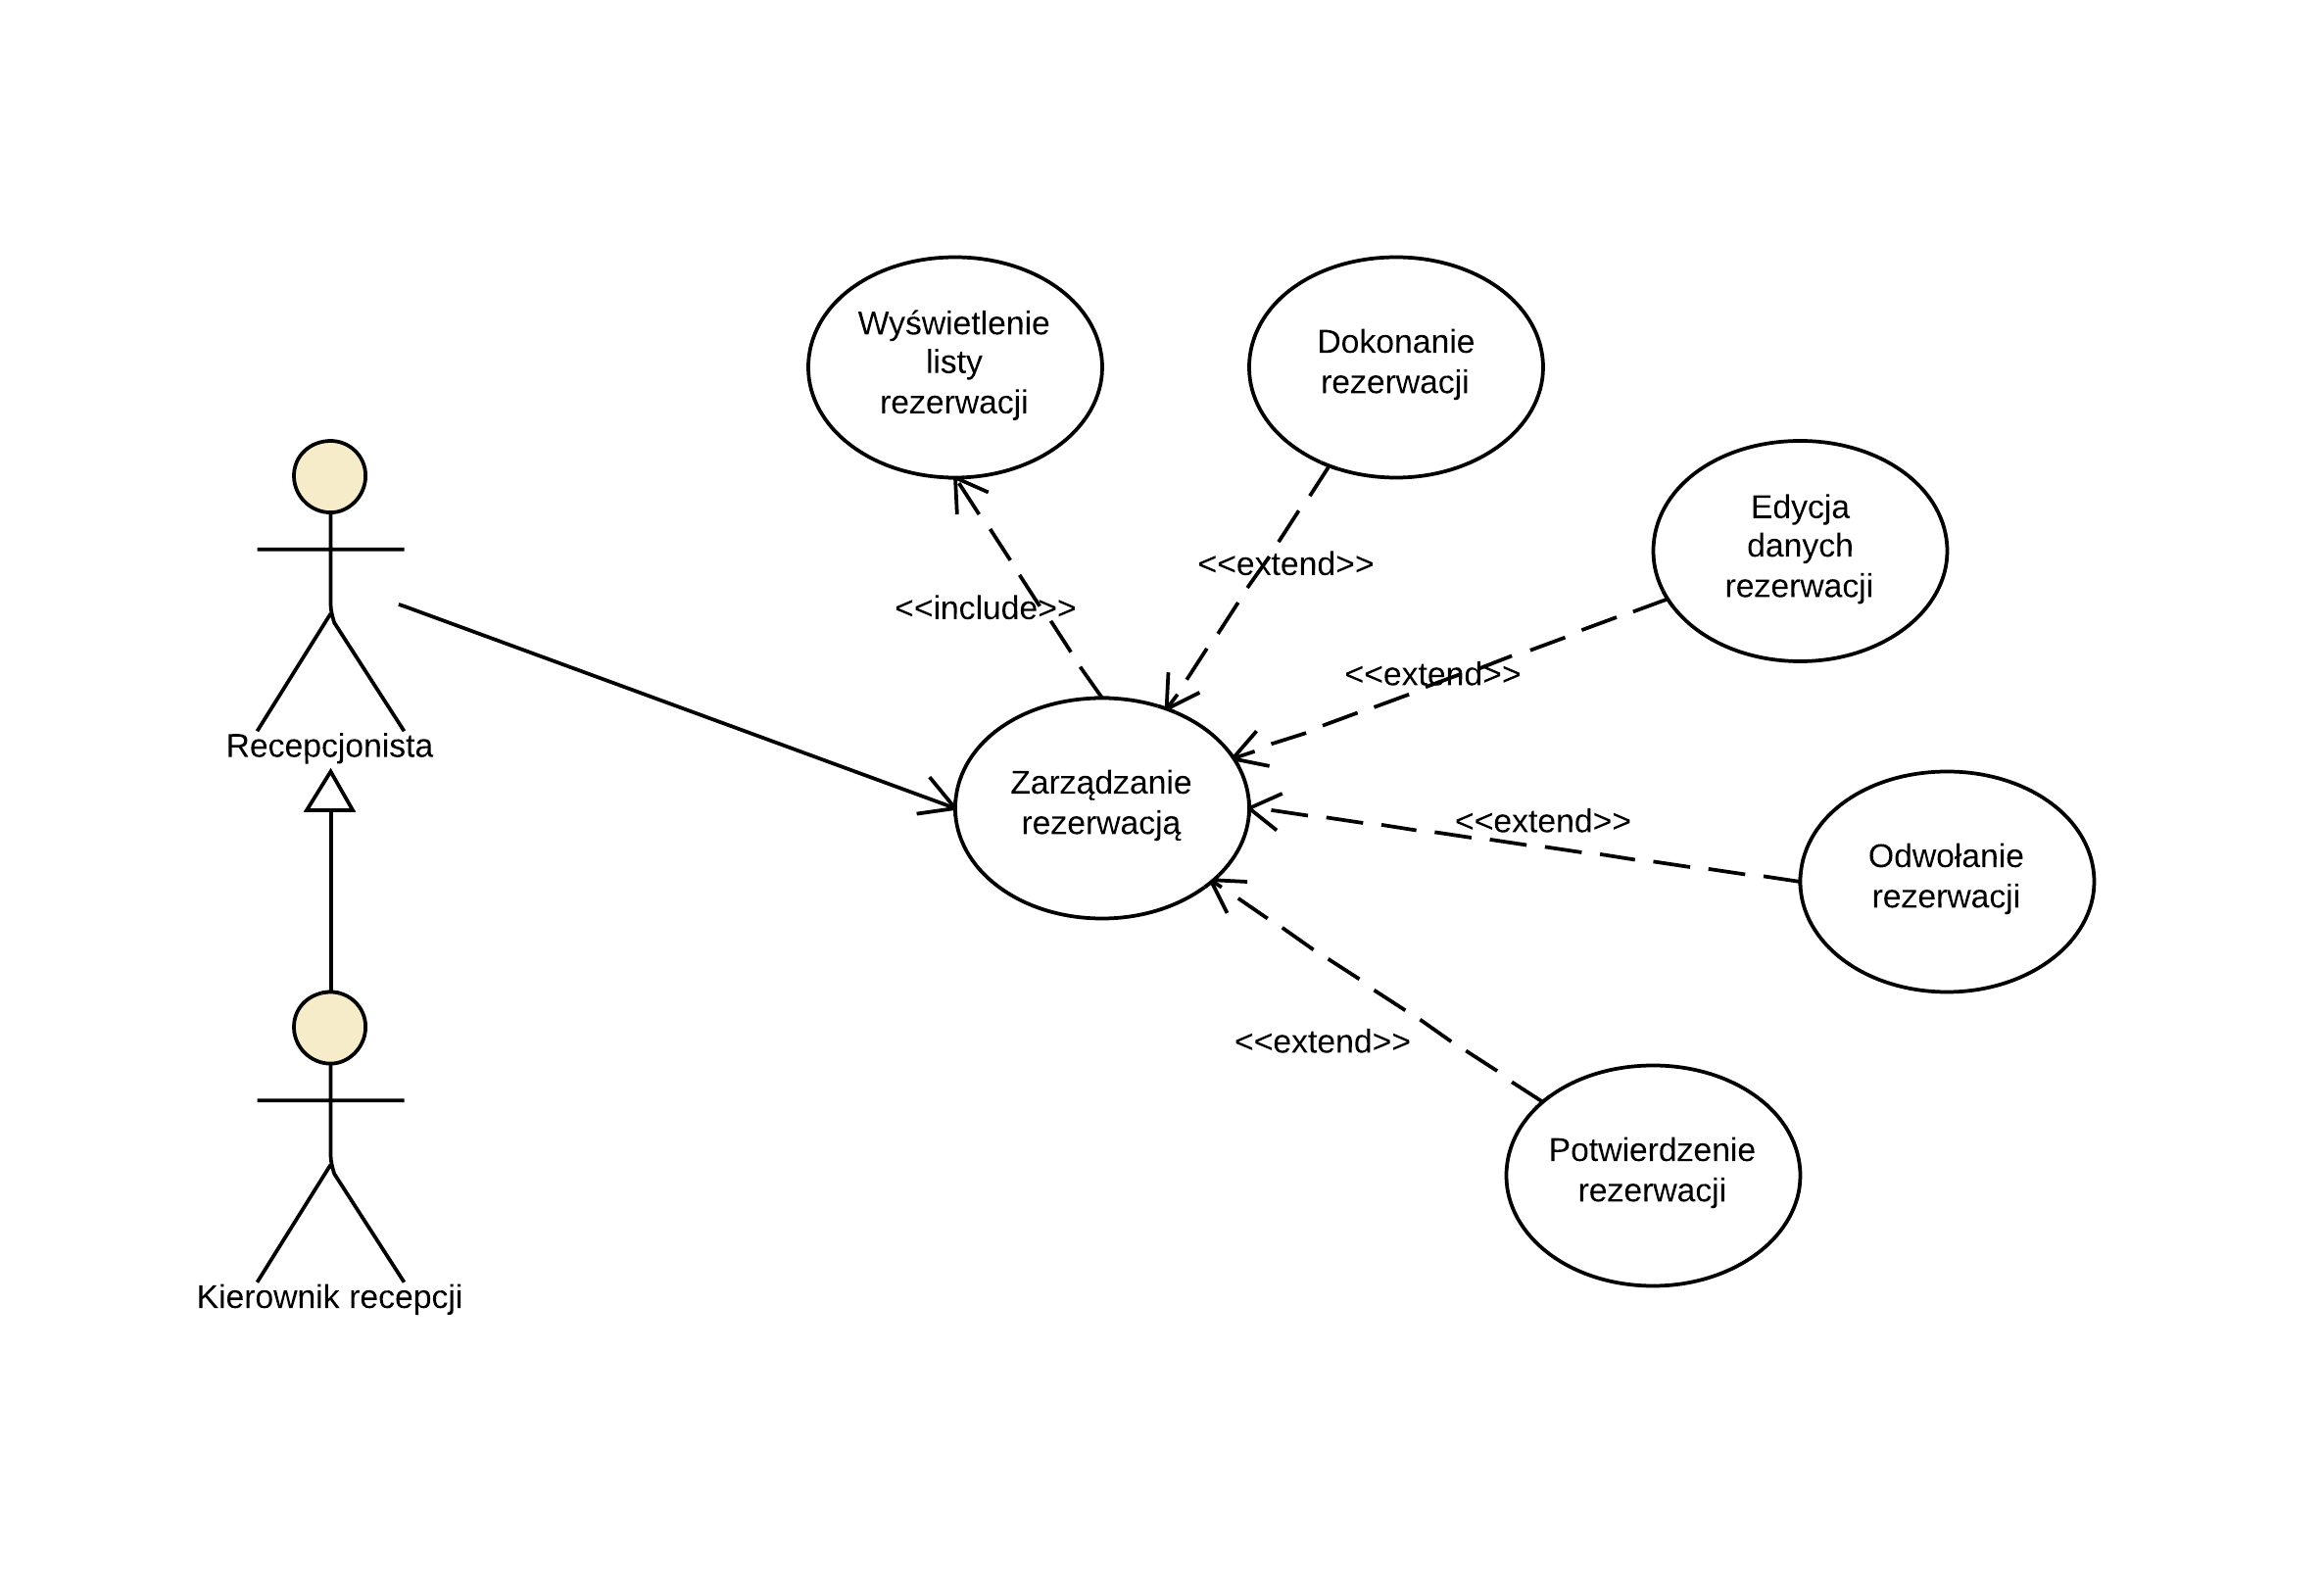
\includegraphics[width=\textwidth]{../img/RezerwacjaUseCase.png}
  }
  \end{center}
  \caption{Przypadki użycia związane z rezerwacją}
  \label{fig:uc-rezerwacja}
\end{figure}

\subsection{Przypadek użycia - Dokonanie rezerwacji}
Ten przypadek użycia pokrywa funkcjonalność, w której rezerwacja dokonywana jest albo telefoniczne, albo osobiście w hotelu.
\begin{description}
  \item [Przypadek użycia] - Dokonanie rezerwacji
  \item [Aktorzy] - Recepcjonista, Klient
  \item [Aktor inicjujący] - Recepcjonista
  \item [Warunki wstępne] - Recepcjonista zalogowany w systemie
  \item [Rezultat] - nowa niepotwierdzona rezerwacja w systemie
\end{description}

\begin{enumerate}
  \item Recepcjonista przechodzi do modułu rezerwacji
  \item Recepcjonista wybiera opcję utworzenia nowej rezerwacji
  \item Recepcjonista wybiera typ rezerwacji
  \item Recepcjonista wybiera datę pobytu
  \item Recepcjonista wybiera typ pokoju
  \item Recepcjonista wybiera stawkę
  \item Recepcjonista szuka klienta w systemie
  \item System nie znajduje klienta 
  \item Recepcjonista uzupełnia część formularza z danymi klienta
  \item Recepcjonista wybiera metodę płatności
  \item Recepcjonista podaje dodatkowe informacje
  \item Recepcjonista wybiera akcję ,,Rezerwuj''
  \item System sprawdza poprawność danych rezerwacji
  \item System informuje recepcjonistę o pomyślnym dodaniu rezerwacji
\end{enumerate}

Scenariusz alternatywny 1: Klient istnieje w systemie

\begin{enumerate}
  \item - 7. tak jak w scenariuszu głównym
  \setcounter{enumi}{7}
  \item System znajduje klienta
  \item Recepcjonista wybiera znalezionego klienta
  \item System automatycznie uzupełnia część formularza z danymi klienta 
  \item Tak jak w scenariuszu głównym od 10.
\end{enumerate}

Scenariusz alternatywny 2: Nie ma wolnych pokoi w wybranym terminie

\begin{enumerate}
  \item - 4. - tak jak w scenariuszu głównym 
  \setcounter{enumi}{4}
  \item Recepcjonista proponuje Klientowi inny typ pokoju dostępny w wybranym terminie pobytu
  \item Klient zgadza się na propozycję
  \item Tak jak w scenariuszu głównym od 6.
\end{enumerate}

\section{Prototypowanie}
Proces prototypowania, nazywany także szybkim makietowaniem, jest bardzo przydatny podczas weryfikacji wymagań i 
projektowania aplikacji. Utworzenie prototypu interfejsu użytkownika pozwala na szybkie wyłapanie błędów i różnych 
braków. Jest to też pierwszy etap, na którym można pokazać klientowi jak wyglądać będzie aplikacja. Należy jednak 
wytłumaczyć klientowi, aby nie skupiał się \mbox{na grafice} oraz wrażeniach estetycznych, chociaż dyskusja na ten temat 
będzie przydatna w późniejszym etapie projektu. Teraz jednak najważniejsza jest weryfikacja wymagań i wyłapanie 
potencjalnych błędów oraz nieporozumień. Ujrzenie nawet bardzo prostego szkicu daje bardzo wiele informacji zarówno 
dla projektantów jak i klienta.

Przed implementacją systemu utworzyłem makiety\footnote{do utworzenia makiet skorzystałem z narzędzia dostępnego pod adresem \url{http://www.balsamiq.com/ }} najważniejszych części systemu. Stworzone makiety dołączone zostały do dodatku \ref{dodatek-makiety}.

Zainteresowanych tematem prototypowania odsyłam do książki o inżynierii oprogramowania autorstwa Krzysztofa Sachy \cite{sacha2010inzynieria} oraz do artykułu na ten temat \cite{wireframes2012infoq}.


\section{Podsumowanie}
W tym rozdziale omówione zostały wybory technologiczne. Każdy wybór posiadał uzasadnienie przedstawione czytelnikowi. Następnie czytelnik poznał proces projektowy aplikacji. W następnym rozdziale omówiony został model danych.

%%%%
%%%% CHAPTER MODEL DANYCH
%%%%

\chapter{Model danych}
Utworzenie modelu danych jest kolejnym etapem projektu po dokonaniu analizy wymagań i wybraniu odpowiednich technologii. Efektem tej pracy jest diagram związków encji.

\section{Model związków-encji}
Model związków-encji przedstawia encje, czyli pewne byty, elementy świata rzeczywistego powiązane z innymi encjami. Powiązania te nazywane są związkami. \mbox{To tylko} krótkie przypomnienie, ponieważ czytelnik powinien być zaznajomiony \mbox{z modelowaniem} encji. 
Model powstał dzięki analizie domeny dziedziny przedstawionej w rozdziale \ref{analiza-dziedziny}, analizie wymagań z rozdziału \ref{wymagania} i makiet z tego samego rozdziału. Diagramy przedstawione zostały przy użyciu notacji Barkera\footnote{nazywaną także notacją Oracle}.

\section{Proces modelowania}
Proces modelowania przebiegał iteracyjnie. W każdej iteracji zachodziły pewne modyfikacje modelu. W idealizowanym świecie wystarczyłoby tylko raz utworzyć model, który później można by zaimplementować. Praktyka pokazuje jednak, że zmiany zachodzą w modelu nawet w późnym etapie projektu. Wraz z większą wiedzą o domenie problemu, wymaganiach klienta, wizja systemu zmienia się. Niektóre z tych zmian wymagają modyfikacji modelu. 

Modele przedstawione w niniejszym rozdziale są ostatnimi, najbardziej dopracowanymi wersjami modeli. Cały model jest zbyt duży, aby pokazać go na jednym diagramie, dlatego też przedstawię model w osobnych częściach.

\section{Model rezerwacji}
Diagram (\ref{fig:db-logical-model-reservation}) przedstawia część modelu związaną z rezerwacją. Najważniejszą encją jest encja rezerwacji. Część encji została uproszczonych. Ich pełne postacie będą przedstawione w kolejnych częściach modelu.

\begin{figure}[H]
  \begin{center}
  \fbox{
    \includegraphics[scale=0.50, angle=270]{../img/rezerwacja-logiczny-v9.pdf}
  }
  \end{center}
  \caption{Model rezerwacji}
  \label{fig:db-logical-model-reservation}
\end{figure}

\subsection{Rezerwacja}
Encja Rezerwacja zawiera informacje dotyczące rezerwacji. Bardzo istotny jest związek rezerwacji z encją Doba. Dzięki temu związkowi, można określić dzień przyjazdu i wyjazdu. Pozwala to także na przedłużenie pobytu oraz praktycznie wszystkie operacje na rezerwacji, takie jak przesunięcie rezerwacji, operacji rozdzielenia rezerwacji, zmiany pokoju na ostatnią dobę. 

\subsubsection{Problem rezerwacji grupowej i pojedynczej}

Podczas modelowania sporym problemem było rozwiązanie kwestii rezerwacji pojedynczej i grupowej. Chcemy osiągnąć taki model, aby:

\begin{enumerate}
  \item łatwo stwierdzić czy rezerwacja jest grupowa, czy pojedyncza
  \item każda rezerwacja była identyfikowana poprzez swój numer rezerwacji - niezależnie od tego, czy jest to grupowa, czy pojedyncza rezerwacja
  \item rezerwacja grupowa powinna być identyfikowana poprzez numer grupy i sekwencję w grupie.
\end{enumerate}

Przedstawię kolejne podejścia do tego problemu. Podczas rozważań poruszam kwestie modelu fizycznego opartego o relacyjną bazę danych. Mam świadomość tego, że w modelu logicznym nie istnieje pojęcie klucza, indeksu i innych terminów z baz danych. 

Pierwsze podejście przedstawione na rysunku poniżej (\ref{fig:db-logical-model-group-reservation-first-try}) pokazuje, że problem został rozwiązany poprzez założenie, że rezerwacja pojedyncza i grupowa to dwa różne podtypy. Można jednak zauważyć, że rezerwacja grupowa, oprócz złożonego identyfikatora składającego się z sekwencji oraz związku z grupą, nie posiada żadnych atrybutów. Obserwacja ta wzbudziła moją wątpliwość. Oprócz tego, taki model wydaje się być trudny w implementacji. Jeśli przyjmiemy realizację tego modelu przy użyciu relacyjnej bazy danych\footnote{postać tabelaryczna to tylko jedna możliwość realizacji modelu fizycznego} to prawdopodobnie każdy podtyp miałby osobną tabele - musiałoby tak być, aby móc stworzyć klucz główny dla rezerwacji grupowej. Powodowałoby to dużo złączeń przy najczęstszej operacji, czyli wyświetlania rezerwacji.

\begin{figure}[H]
  \begin{center}
  \fbox{
    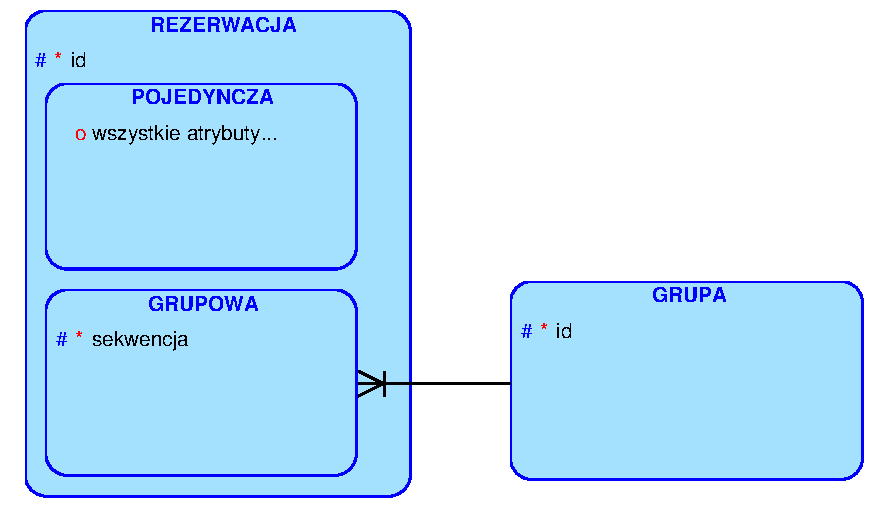
\includegraphics[width=200px]{../img/podejscie1.pdf}
  }
  \end{center}
  \caption{Pierwsze podejście do problemu rezerwacji grupowej i pojedynczej}
  \label{fig:db-logical-model-group-reservation-first-try}
\end{figure}

Drugie podejście do problemu korzysta z obserwacji, że rezerwacja tak naprawdę nie składa się z podtypów, a jest jednym bytem. To czy rezerwacja jest grupowa wynika z tego, czy rezerwacja należy do grupy, czy też nie. W tym podejściu podejrzanym wydaje się związek typu jeden-do-jeden, który sygnalizuje zbyt duży podział. 

\begin{figure}[H]
  \begin{center}
  \fbox{
    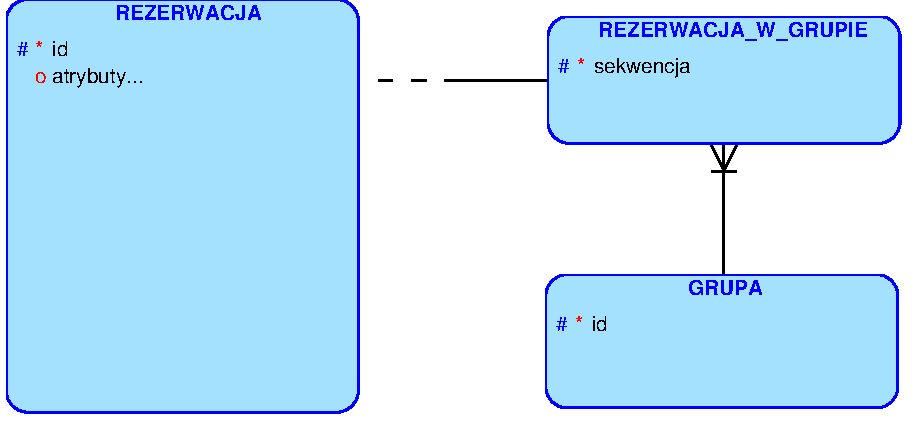
\includegraphics[width=200px]{../img/podejscie2.pdf}
  }
  \end{center}
  \caption{Drugie podejście do problemu rezerwacji grupowej i pojedynczej}
  \label{fig:db-logical-model-group-reservation-second-try}
\end{figure}

Kolejne podejście pozbywa się podejrzanego związku jeden-do-jeden, ale zyskujemy dziwny identyfikator. Logika za tym identyfikatorem jest taka, że sekwencja dla rezerwacji pojedynczej ma wartość zero, a dla grupowej taką jak sekwencja \mbox{w grupie} licząc od jednego. Ta komplikacja kompromituje model. Aby ten model spełniał wymagania, należałoby także dodać odpowiednie warunki na obowiązkowość związku i wartość sekwencji. Można by się pozbyć warunku, zmieniając związek na obustronnie obligatoryjny i użyć specjalnej instancji encji Grupa, która oznaczałaby, że grupa nie istnieje. Ten model wprowadza zbyt dużo komplikacji, dlatego szukałem czegoś prostszego.

\begin{figure}[H]
  \begin{center}
  \fbox{
    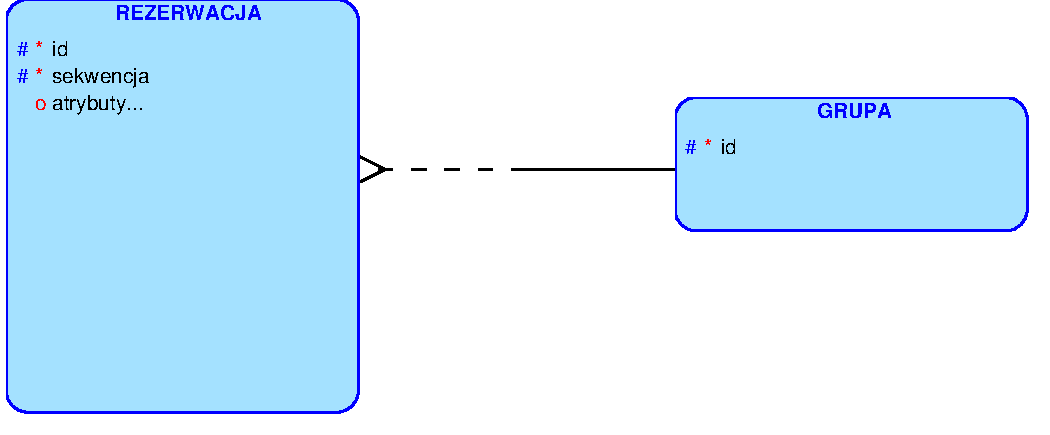
\includegraphics[width=200px]{../img/podejscie3.pdf}
  }
  \end{center}
  \caption{Trzecie podejście do problemu rezerwacji grupowej i pojedynczej}
  \label{fig:db-logical-model-group-reservation-third-try}
\end{figure}

W czwartym podejściu odrzucam sekwencję z identyfikatora, dzięki czemu pozbawiam się komplikacji związanych ze specjalnymi wartościami. Powstał nowy atrybut o nazwie ,,czy grupowa'', którego nazwa dość dobrze sygnalizuje za co odpowiada. Model nie ogranicza rezerwacji w związku z grupą bez numeru sekwencji, dlatego też należałoby to wymusić odpowiednim warunkiem w modelu fizycznym. Plusem tego modelu jest to, że od razu wiadomo, czy rezerwacja jest pojedyncza czy grupowa. 

Przyglądając się bliżej stwierdziłem, że ten atrybut jest redundantny, ponieważ \mbox{z samego} faktu istnienia związku między rezerwacją, a grupą wynika to czy rezerwacja jest grupowa czy pojedyncza. W kolejnym, piątym podejściu, atrybut ten został wyeliminowany.

\begin{figure}[H]
  \begin{center}
  \fbox{
    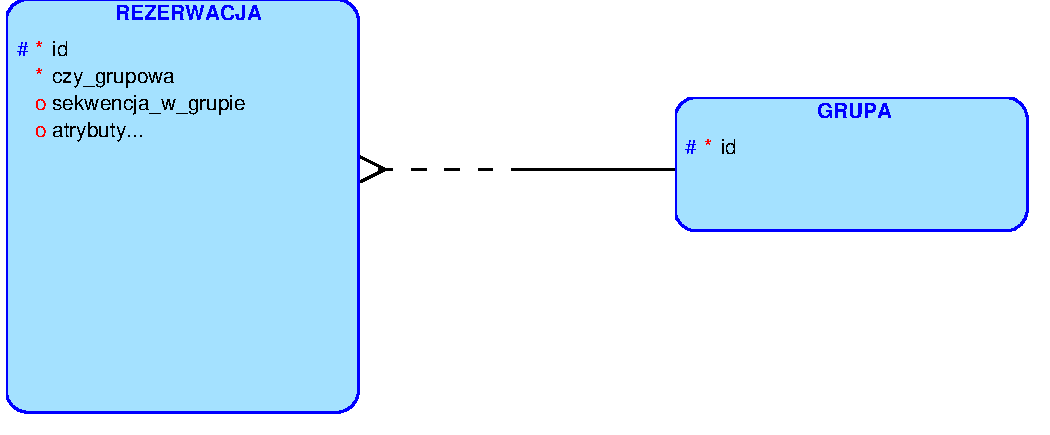
\includegraphics[width=200px]{../img/podejscie4.pdf}
  }
  \end{center}
  \caption{Czwarte podejście do problemu rezerwacji grupowej i pojedynczej}
  \label{fig:db-logical-model-group-reservation-fourth-try}
\end{figure}

\begin{figure}[H]
  \begin{center}
  \fbox{
    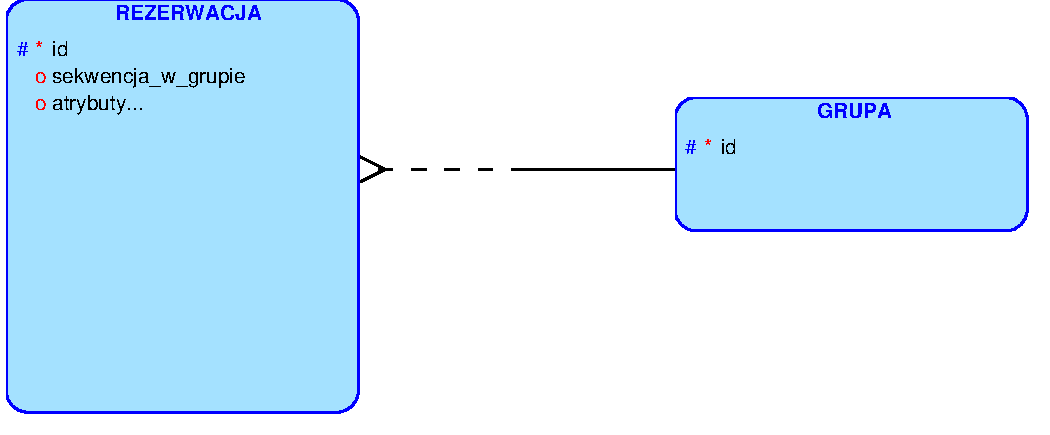
\includegraphics[width=200px]{../img/podejscie5.pdf}
  }
  \end{center}
  \caption{Piąte podejście do problemu rezerwacji grupowej i pojedynczej}
  \label{fig:db-logical-model-group-reservation-fifth-try}
\end{figure}

Widząc końcowy efekt, bardzo łatwo powiedzieć, że rozwiązanie jest trywialne. Jest to pewien sukces modelu. Czytelnik mógłby się zastanawiać, dlaczego nie osiągnąłem tego modelu w pierwszym podejściu. Wynika to z analizy dziedziny. Analizując dziedzinę miałem przeświadczenie, że rezerwacja ma dwa typy - rezerwacja grupowa i rezerwacja pojedyncza. Stąd też w pierwszym podejściu model \mbox{z podtypami}. Dla tego modelu konieczny jest warunek wymuszający obligatoryjność sekwencji w grupie jeśli zachodzi związek między rezerwacją i grupą. Dodatkowo, aby spełnić wymaganie 3. należy utworzyć indeks na sekwencji i kluczu, jaki powstanie ze związku. Zadając pytania i zastanawiając się nad sensownością modelu udało się otrzymać prosty model, który spełnia wymagania.

\subsection{Usługa}
Encja usługa pozwala na realizację usługi typu budzenie na życzenie oraz innych usług, które muszą być zrealizowane w pewnym czasie. Nie ma dobrego naturalnego identyfikatora dla usługi, dlatego też jest to sztuczny identyfikator.

\subsection{Typ usługi}
Encja typ usługi jest encją słownikową. Określa dziedzinę możliwych w realizacji usług wraz ze standardową cenę za usługę. Jednym z typów usługi, może być ,,usługa inna'', która pozwoli na realizację nietypowej usługi żądanej przez klienta.

\subsection{Doba}
Encja doba jest istotna, ponieważ pozwala na dużą dowolność w przebiegu pobytu gościa w hotelu. Rezerwacja na 10 dni, składać się będzie z 10 dób, gdzie każda doba mogłaby być spędzona w innym pokoju. Jest to oczywiście ekstremalny przypadek, ale zmiana pokoju na ostatnią dobę jest dość często spotykana \mbox{w hotelarstwie}.

\subsection{Status doby}
Encja status doby jest encją słownikową. Może zawierać takie wartości jak: użyta doba, nieużyta doba, doba ekstra lub inne. To, czy ta encja jest potrzebna, jest kwestią dyskusyjną, tak jak każda decyzja podczas modelowania.

\subsection{Status rezerwacji}
Encja status rezerwacji jest encją słownikową i określa możliwe statusy rezerwacji, jakie poznaliśmy podczas analizy dziedziny. Dodatkowo te statusy mogą być rozszerzone o parę technicznych statusów.

\subsection{Osoba}
Encja osoba modeluje osobę, która może być gościem i/lub właścicielem rezerwacji bądź grupy. Osoba może mieć tożsamość prawną lub być osobą fizyczną czyli gościem. Dodatkowo model zakłada istnienie podtypu Pracownika, który jest przydany przy realizacji aplikacji. 

\subsection{Adres}
Encja adres modeluje adres osoby. Ważny jest związek z typem adresu, który określa czy adres jest główny, drugorzędny, korespondencyjny, kontaktowy, czy do płatności. Same atrybuty w encji adres nie są wystarczające do ustalenia pełnego adresu, dlatego też obowiązkowy jest identyfikujący związek z encją kraj, która przedstawia dane specyficzne dla kraju. Encja kraj to też swojego rodzaju encja słownikowa, ponieważ docelowo powinna zawierać dane wszystkich krajów na świecie.

\subsection{Metoda obciążenia}
Encja metoda obciążenia określa kto powinien płacić za rezerwację. Możliwymi opcjami są: właściciel rezerwacji, gość lub właściciel z limitem. Właściciel rezerwacji to metoda, która wybrana będzie, gdy rezerwacja będzie w ofercie biura podróży. Gość to metoda w przypadku rezerwacji pojedynczej przez osobę indywidualną. Właściciel rezerwacji może płacić za wszystkie rezerwacje w grupie lub płacić tylko z limitem. Za koszta przewyższające określony limit odpowiada gość. 

\subsection{Podsumowanie}
Model rezerwacji pozwala na stworzenie rezerwacji pojedynczej, grupowej, określenie właściciela rezerwacji, określenia korzystających z rezerwacji gości, bardzo dokładnego określenia przebiegu pobytu, modyfikacji pobytu, świadczenia usług, identyfikacji gości przy kolejnych wizytach i wgląd w ich historie. Model ten spełnia postawione mu wymagania.


\section{Model stawek}
Model stawek zawiera encje, które pozwalają na dokładne określenie stawek na pokój. 


\begin{figure}[H]
  \begin{center}
  \fbox{
    \includegraphics[scale=0.6, angle=270]{../img/stawki-logiczny-v7.pdf}
  }
  \end{center}
  \caption{Model stawek}
  \label{fig:db-logical-model-rates}
\end{figure}

\subsection{Stawka}
Encja stawka określa stawki na pokoje. Encja posiada sztuczny identyfikator. Encja stawka umożliwia określenie następujących stawek z dokładnością co \mbox{do pokoju}:

\begin{itemize}
  \item stawka rack dla typów osób, np. stawka rack dla klientów indywidualnych
  \item stawka rack dla konkretnych osób, np. stawka dla klienta stałego
  \item stawka sezonowa dla typów osób
  \item stawka sezonowa dla konkretnych osób
  \item stawka pakietowa dla typów osób
  \item stawka pakietowa dla konkretnych osób
\end{itemize}

\subsubsection{Stawka pakietowa}
Stawka pakietowa jest związana z dobą pakietową (\ref{noc-pakietowa}), która dalej jest związana z pakietem, który sam w sobie stanowi całą ofertę dla pobytu. Przykład takiego pakietu poznaliśmy podczas analizy dziedziny (\ref{pakiet-walentynki}). Stawka pakietowa stanowi konkretną cenę na pokój dla danego pakietu. Model pakietu został jest przedstawiony w osobnej części modelu (\ref{model-pakietu-i-dodatkow}).

Encja stawka daje ogromne możliwości w określaniu stawek i spełnia wszystkie wymagania dotyczące określania stawek na pokoje. 

\subsection{Typ osoby}
Związek osoby z typem osoby nie był widoczny na poprzednim modelu. Encja typ osoby jest encją słownikową i pozwala rozróżnić czy dana osoba jest klientem indywidualnym, klientem korporacyjnym czy klientem innego rodzaju. 

\subsection{Rack}
Encja rack jest encją potrzebną do ustawienia stawek typu rack. Encja rack jest identyfikowana poprzez kod oraz związek z pokojem. Częstą praktyką jest nadawanie stawkom rack kodów typu RACK100 lub RACK500. Atrybut kod pozwala \mbox{na nadawanie} nazw kodowych stawkom.

\subsection{Sezon}
Encja sezon pozwala na określanie stawek ograniczonych czasowo. Encja sezon posiada sztuczny identyfikator. Sezonem może być np. sezon świąteczny, wakacyjny. Można także użyć sezonu do określenia stawek na wszystkie weekendy pomiędzy styczniem, a marcem dla klientów indywidualnych. Encja sezon spełnia wymagania związane z stawkami sezonowymi i daje bardzo dużą elastyczność \mbox{w określeniu} konkretnych przedziałów czasowych.

\subsection{Okres czasu}
Encja okres czasu modeluje odcinek czasu, w którym dana stawka jest dostępna. Choć para dat jest kandydatem na identyfikator, to zbudowanie identyfikatora w ten sposób powodowałoby, że niemożliwe było by utworzenie stawki pakietowej i sezonowej dostępnej w tym samym okresie czasu. Z tego powodu okres czasu musi mieć sztuczny identyfikator.

\subsection{Pokój}
Encja pokój reprezentuje fizyczny pokój w hotelu. Pokój posiada naturalny identyfikator i jest to numer pokoju. Pokój posiada informacje o tym, czy jest zajęty, ile mieści osób standardowo oraz maksymalnie, ile może być dodatkowych łóżek. Posiada, także prefiks, który wraz z numerem pokoju stanowi nazwę pokoju.

\subsection{Typ Pokoju}
Encja typ pokoju jest encją słownikową i określa możliwe typy pokojów.

\subsection{Status pokoju}
Encja status pokoju jest encja słownikową i określa status pokoju związany ze służbą pięter. Możliwe statusy to m.in. czysty pokój, brudny, nieczynny, remont.

\subsection{Podsumowanie}
Model stawek pozwala na precyzyjne określenie stawek dla typów osób jak również dla konkretnych osób. Dzięki temu możliwe są operacje na całych grupach, np. obniżka wszystkich stawek RACK dla klientów indywidualnych jak również określenie specjalnej stawki dla stałego klienta.


\section{Model pakietu i dodatków}
\label{model-pakietu-i-dodatkow}
W tej części modelu przedstawione zostaną encje, które częściowo były widoczne w części modelu rezerwacji. Model przedstawiony został na rysunku \ref{fig:db-logical-model-package}.

\begin{figure}[H]
  \begin{center}
  \fbox{
    \includegraphics[scale=0.6, angle=270]{../img/pakiet-logiczny-v6.pdf}
  }
  \end{center}
  \caption{Model pakietu i dodatków}
  \label{fig:db-logical-model-package}
\end{figure}

\subsection{Pakiet}
Encja pakiet umożliwia definiowanie pakietów na grupę dodatków np. obiad \mbox{i kolacja} jak również na definiowanie pakietów definiujących cały pobyt i cenę każdej doby z osobna. Pakiet nie ma naturalnego identyfikatora, dlatego też został użyty sztuczny identyfikator.

To, czy pakiet jest pakietem na pobyt czy tylko zgrupowanymi dodatkami, wynika z istnienia związków, w jakie wchodzi konkretny pakiet. Jeśli pakiet wchodzi \mbox{w związek} \mbox{z dobą} pakietową, to jest to pakiet na pobyt. Skorzystanie z takiego pakietu będzie możliwe jedynie poprzez zdefiniowanie stawek dla tego pakietu. Możliwe jest precyzyjne definiowanie stawek na każdą dobę w pakiecie.

Warto zauważyć, że pakiet dodatków będzie miał taką samą cenę dla każdego gościa, niezależnie od jego typu. W przypadku pakietu z pobytem korzystamy \mbox{z bogactwa} encji stawka, która pozwala określać stawki na typy osób oraz konkretne osoby.

Pakiet może być dostępny tylko w określonym czasie. Tą funkcjonalność realizuje związek z okresami czasu.

\subsection{Doba pakietowa}
\label{noc-pakietowa}
Encja doba pakietowa pozwala na określenie ceny dla każdej doby z osobna \mbox{na każdy} pokój w ofercie pakietu z pobytem. Taka precyzja pozwala na budowanie wyrafinowanych ofert. Encja jest encją słabą identyfikowaną poprzez związek \mbox{z pakietem} oraz sekwencję.

\subsection{Dodatek}
Encja dodatek określa cenę, nazwę i maksymalną zniżkę na dany produkt (\ref{model-produkt}). Każdy dodatek ma określony sposób realizacji oraz sposób kalkulacji opłaty za dodatek. Encja dodatek posiada sztuczny identyfikator.

\subsection{Sposób kalkulacji}
Encja sposób kalkulacji pozwala na określenie w jaki sposób powinna być kalkulowana opłaca za dodatek. Możliwe sposoby kalkulacji to m.in. \mbox{na osobę}, \mbox{na pokój}, \mbox{na dorosłego}. Encja ta jest encją słownikową.

\subsection{Sposób realizacji}
Encja sposób realizacji umożliwia określenie tego kiedy dodatek ma zostać zrealizowany. Możliwe sposoby realizacji zostały zdefiniowane w punkcie \ref{sposob-realizacji} w wymaganiach funkcjonalnych (\ref{wymagania-funkcjonalne}).

\subsection{Produkt}
\label{model-produkt}
Encja produkt definiuje produkt, który może być użyty jako dodatek. Takim produktem jest np. obiad, gazeta, kwiaty. Produkt może mieć także charakter użycia usług fakultatywnych np. skorzystanie z basenu. Encja produkt posiada sztuczny identyfikator.

\subsection{Kupiony pakiet}
Encja kupiony pakiet jest encją powstałą ze związku rezerwacji i pakietu. Wartość atrybutu ceny, może różnić się od tej zdefiniowanej w pakiecie z powodów zniżek, umiejętności negocjacyjnych klienta lub uprzejmości obsługi hotelu. Atrybut o nazwie timestamp jest częścią identyfikatora, aby umożliwić zakup wielu takich samych pakietów i śledzić ich czas zakupu.

\subsection{Kupiony dodatek}
Encja kupiony dodatek ma sens analogiczny do encji kupiony pakiet.

\subsection{Podsumowanie modelu pakietów i dodatków}
Model pakietów oraz dodatków pozwala na budowanie wyrafinowanych ofert pobytowych z precyzyjnie określonymi stawkami oraz sprzedaż usług dodatkowych \mbox{z określonymi} sposobami dostarczania i kalkulacji ceny dodatków do pobytu. Model ten umożliwia spełnienie wymagań dotyczących dodatków oraz pakietów.

\section{Podsumowanie modelu logicznego}
W tym rozdziale przedstawiłem model logiczny aplikacji. Przedstawiłem także przykładowy proces myślowy i rozważania nad modelowaniem konkretnego problemu. Pozostała część modelu powstała w oparciu o podobne rozważania i szukanie coraz lepszego, prostszego, bardziej ekspresywnego modelu, który spełni wymagania. Całość modelu logicznego została dołączona do dodatku \ref{dodatek-model-logiczny}. W rezultacie modelowania powstał przejrzysty model mogący spełnić wszystkie wymagania.

\chapter{Implementacja}
W niniejszym rozdziale przedstawione zostały wybrane elementy implementacji systemu. Zacząłem od omówienia modelu fizycznego, a następnie omówiłem parę elementów z wyższych warstw aplikacji. 

\section{Fizyczny model danych}
Fizyczny model danych, w tym przypadku tabelaryczny model danych, powstał poprzez przekształcenie modelu związków encji do postaci tabelarycznej. Model ten został przedstawiony na rysunku \ref{fig:db-physical-model}.

Proces wymagał podjęcia pewnych decyzji. Oprócz standardowych działań, jak wprowadzenie dodatkowej tabeli w miejsce związku wiele do wiele, należało zdecydować się na sposób implementacji podtypów. Postanowiłem zastosować technikę jednej tabeli z dyskryminatorem określającym typ oraz warunkami wymuszającymi obligatoryjność atrybutów w zależności od wartości dyskryminatora. Za tą metodą przemawia brak złączeń, a więc wydajność kosztem miejsca.

Implementacja łuków została osiągnięta poprzez opcjonalne klucze obce z warunkami sprawdzającymi zajście tylko jeden relacji i wykluczanie pozostałych.

Kolejność kolumn w tabelach ma znaczenie. Dobrą praktyką jest uporządkowanie kolumn w zależności od najmniejszej znanej długości oraz według obligatoryjności. Oznacza to, że wymagana wartość w kolumnie o typie CHAR, będzie wcześniej niż wymagana wartość w kolumnie o typie VARCHAR2. Dzięki takiej kolejności oszczędza się miejsce w bazie danych.

\subsection{Klucze}
Podobne znaczenie ma kolejność kolumn w złożonych kluczach głównych, \mbox{w których} część klucza jest kluczem obcym. Umieszczając te klucze obce, które są częścią klucza głównego przed resztą klucza zyskujemy darmowy indeks na ten klucz obcy.

Na wszystkie klucze obce zostały nałożone indeksy nieunikalne. Indeksy nieunikalne założone zostały, aby umożliwić szybkie złączenia. 

Indeks unikalny został zastosowany, aby w tabeli rezerwacji nie było dwóch rezerwacji, które należą do takiej samej grupy i mają taką samą sekwencję. \mbox{Na rysunku} \ref{fig:db-physical-model} jedyne indeksy unikalne to te, których nazwa kończy się na ,,UNIQUE\_\_IDX''.

W większość tabel zostały użyte sztuczne identyfikatory generowane z sekwencji. Jedynie tabela pokoje zawiera naturalny klucz główny. Tabele powstałe z encji słownikowych posiadają klucze główne zbudowane ze swoich atrybutów.

\subsection{Złączenie klucza}
Wartym odnotowania jest złączenie klucza obcego w tabeli stawki. Tabela stawki posiada klucz obcy z numerem pokoju oraz klucz obcy do tabeli racks, który składa się z numeru pokoju oraz kodu rack. Gdyby nie złączenie klucza, to tabela stawki posiadała by trzy kolumny\footnote{pomijam konieczność dodania prefiksu, aby nazwy były różne}:
\begin{itemize}
  \item numer pokoju - klucz obcy do tabeli pokoje,
  \item numer pokoju - część klucza obcego do tabeli racks,
  \item kod - część klucza obcego do tabeli racks.
\end{itemize}

Złączenie numeru pokoju w jedną kolumnę i użycie jej w obu kluczach obcych uniemożliwia zdefiniowanie stawki rack dla pokoju innego niż ten sam pokój. Gdyby istniały dwie kolumny z numerem pokoju, to byłoby to możliwe. Można by temu zapobiec wymagając równości wartości w tych kolumnach poprzez dodatkowy warunek lub poprzez logikę aplikacji. Złączenie kolumn jest jednak najbardziej eleganckim rozwiązaniem.


% \begin{figure}[H]
%   \begin{center}
%   \fbox{
%     \includegraphics[scale=0.25, angle=270]{../img/model-fizyczny-v4.pdf}
%   }
%   \end{center}
%   \caption{Model fizyczny bazy danych}
  
% \end{figure}

\clearpage
 {\pdfpagewidth=2\pdfpagewidth
    \vspace*{1cm}
    \noindent\kern.5\pdfpagewidth\rlap{\parbox{\textwidth}{%
    \noindent\kern.25\pdfpagewidth
        \llap{\includegraphics[width=308mm,height=209mm,page=1]{../img/model-fizyczny-v4.pdf}\label{fig:db-physical-model}}\endgraf
    \vspace{2ex}%
    \captionof{figure}{Model fizyczny bazy danych}}}\kern-.5\pdfpagewidth
     \par
     \vspace*{-5cm}
\clearpage
}


\section{Dostęp do danych}
Tradycyjną metodą dostępu do danych jest mapowanie na obiekty typu POJO\footnote{ang. Plain Old Java Object}, czyli proste obiekty javowe, pozbawione zależności od inwazyjnych szkieletów aplikacyjncych. Obiekty POJO zawierają pola oraz metody, które w większości są metodami typu ,,getXXX'' oraz ,,setXXX''. Następnie, aby zaimplementować typową funkcjonalność zapisywania, odczytów, aktualizacji oraz usuwania obiektów stosuje się wzorzec DAO\footnote{ang. Data Access Object}, który zapewnia tę podstawową funkcjonalność.

Niestety, takie podejście prowadzi do tzw. anemicznego modelu. Oznacza, \mbox{to że} obiekty są tylko kontenerami na dane, a logika z nimi związana jest rozproszona \mbox{w wielu} innych miejscach. Zainspirowany podejściem budowy bogatego modelu \cite{evans2004domain} postanowiłem wzbogacić POJO o logikę biznesową oraz zwiększyć ich obiektowość poprzez użycie tzw. obiektów-wartości\footnote{ang. value objects}. Różnicę przedstawiają niniejsze wydruki fragmentu klasy reprezentującej pokój. Aby uniknąć anemicznego modelu domeny warto jest pozbyć się wszystkich metod typu ,,setXXX'' i zastąpić je metodami, które mają znaczenie biznesowe. Przykładowo zamiast ustawiać status rezerwacji metodą ,,setReservationStatus(status)'' lepiej jest utworzyć kilka metod, których efektem ubocznym będzie zmiana statusu rezerwacji. Takimi metodami mogą być np. ,,checkin()'', ,,checkout()''. Wówczas obiekt ma szansę zadbać o to, aby wszystkie jego inwarianty pozostały spełnione. W tym przypadku może to być prawidłowa zmiana statusu. W momencie, gdy enkapsulacja jest utracona poprzez publicznie dostępne metody ,,setXXX'' obiekt może być wprowadzony w niepoprawny stan.

Podobne zagrożenie występuje ze strony metod ,,getXXX'' zwracających mutowalne\footnote{mogące zmienić swój stan} obiekty. Metodą obrony przed tym jest albo defensywne programowanie poprzez tworzenie kopii obiektów, albo używanie niemutowalnych obiektów\footnote{ang. immutable objects.}. Każda zmiana w niemutowalnym obiekcie powoduje utworzenie nowego obiektu. Taki obiekt może być zatem swobodnie udostępniany bez potrzeby kopiowania.

Posiadając bogaty model można posługiwać się terminami DDD. Obiekty posiadające tożsamość w nomenklaturze DDD nazywa się encjami. Obiekty, które posiadają inne encje oraz obiekty-wartości nazywa się agregatami. Agregatem jest np. rezerwacja, pokój i gość.

\begin{lstlisting}[language=Java,style=outcode,caption=anemiczne POJO]
public class Room
{
    private String prefix; 
    private String name;
    private String type;
    private Set<Rate> rates;
    private String housekeepingStatus;
    private String availability;
    private int maxExtraBeds;
    private int standardOccupancy;
    private int maximumOccupancy;

    // ...
}
\end{lstlisting}

\begin{lstlisting}[language=Java,style=outcode,caption=Agregat]
public class Room
{
    private String prefix; 
    private RoomName name;
    private RoomType type;
    private Set<Rate> rates;
    private HousekeepingStatus housekeepingStatus;
    private RoomAvailability availability;
    private Integer maxExtraBeds;
    private Occupancy occupancy;

    // ...
}
\end{lstlisting}

\subsection{Repozytorium zamiast DAO}
W nomenklaturze DDD występuję pojęcie ,,repozytorium''. Jest do kontrakt, który zawiera bogatszy zestaw metod niż tylko te, które są potrzebne do realizacji operacji CRUD\footnote{ang. Create Read Update Delete} tak jak w przypadku obiektów typu DAO. Metody te mają sens biznesowy. Model domeny posługuje się interfejsem do realizacji logiki biznesowej. Implementacja repozytoriów jest niezależna od modelu domeny. W przypadku tej aplikacji repozytoria zostały zaimplementowane przy użyciu biblioteki Hibernate. Przykład kontraktu odpowiedzialnego za działania na rezerwacji został przedstawiony na niniejszym wydruku.

\begin{lstlisting}[language=Java,style=outcode,caption=Repozytorium rezerwacji]
public interface ReservationRepository
{
    Collection<Reservation> findAllReservationsAroundDates(DateTime checkIn,
       DateTime checkOut);

    void bookNewReservation(Reservation reservation);

    Collection<Reservation> getAll();

    Optional<Reservation> lookup(Id id);

    void deleteReservation(Reservation reservation);

    void update(Reservation reservation);
}
\end{lstlisting}

\section{Praktyki programistyczne}
Podczas implementacji aplikacji dużą wagę przywiązałem do dobrych praktyk programistycznych. Stosowałem wzorce projektowe poznane w tradycyjnej książce autorstwa gangu czworga \cite{gamma1994design}. Stosowałem także wskazówki zawarte w książce ,,Effecitve Java'' \cite{bloch2008effective}, a szczególnie wskazówkę nr 15, która zaleca minimalizację użycia obiektów zmieniających stan i faworyzacji niezmiennych obiektów.

\subsection{Obiekty DTO}
Oprócz typowych wzorców, jak fabryka, kompozyt, strategia jest wzorzec warstwy obiektów DTO\footnote{ang. Data Transfer Object}, czyli obiektów transferujących dane. Obiekty DTO zostały zastosowane w warstwie prezentacji w komunikacji pomiędzy serwerem a klientem. Przyjętym formatem wymiany danych jest JSON. Dzięki bibliotece Jersey programista jest uwolniony od konwersji obiektów na odpowiedni format. Dzięki stosowaniu odpowiedniego formatu usługi internetowe mogą przyjmować obiekty DTO, a nie proste typy. Wysłane żądanie, które zawiera obiekt w formacie JSON zostaje przekształcone na odpowiedni obiekt DTO. Pozwala to na eleganckie tworzenie usług internetowych, które konsumują obiekty DTO i produkują obiekty DTO.

\section{Testowanie}
Nieodłącznym elementem pracy nad implementacją było testowanie. Korzystając ze wskazówek zawartych w książce ,,Practical Unit Testing with TestNG and Mockito'' \cite{kaczanowski2012practical} pisałem testy jednostkowe używając nowoczesnych narzędzi. Testy jednostkowe były prawdziwie jednostkowe, a zatem testowany obiekt, był uwolniony od jakichkolwiek innych obiektów i dzięki temu był testowany w całkowitej izolacji. Wszystkie jego zależności były wstrzykiwane podczas testu. Dzięki kodowaniu do interfejsów, a nie do konkretnych klas, łatwo jest wstrzykiwać zaślepki oraz szpiegów do testowanego obiektu w celu sprawdzenia jego działania. Aby to było możliwe, należało tworzyć luźno powiązane komponenty, co jest kolejną dobrą praktyką programistyczną.

Oprócz testów jednostkowych tworzyłem testy integracyjne. Testy integracyjne obejmowały interakcję z bazą danych. Testy pokrywały implementacje repozytoriów i sprawdzały zmiany w bazie danych. 

\chapter{Podsumowanie}

\section{Wnioski}
Wynikiem tej pracy jest kompletny projekt modelu systemu oraz jego częściowa implementacja w postaci działającego i funkcjonalnego prototypu aplikacji. Zaprojektowany system spełnia wszystkie postawione mu wymagania. System pozwala na tworzenie rezerwacji pojedynczej i grupowej, zarządzanie informacjami gości, tworzenie stawek rack, sezonowych i pakietowych dla określonych osób lub/i typów osób, zarządzanie pokojami oraz sprzedaż usług dodatkowych.

Prototyp aplikacji pozwala na dokonywanie rezerwacji pojedynczej według stawek rack i stawek sezonowych, przeprowadzenie prostego audytu nocnego, zarządzanie informacjami gości, łatwy podgląd obłożenia hotelu, przyjazdów, wyjazdów i statystyk hotelu. Prototyp aplikacji nadaje się do użytku dla małego zakładu hotelarskiego. W przypadku pełnej implementacji powstałby zaawansowany produkt użyteczny dla średniej wielkości hotelu.

Decyzje dotyczące wyboru konkretnych technologii okazały się bardzo trafne. Wybrane technologie pozwoliły na stworzenie nowoczesnej, przyjaznej dla użytkownika, całkowicie dynamicznej, zapewniającej bogate doświadczenia podczas użytkowania, funkcjonalnej i łatwo rozwijalnej aplikacji. Cel pracy został osiągnięty.

\section{Dalszy rozwój}
Dalszy rozwój systemu powinien obejmować implementację rezerwacji grupowych, obsługę wszystkich typów klientów, generowanie raportów, zarządzanie pakietami i dodatkami, obsługę stawki pakietowej oraz wsparcie dla służby pięter. Należałoby także zrealizować publiczną część systemu i umożliwić wystawianie ofert pakietowych w internecie oraz dokonywanie rezerwacji on-line. Ważnym elementem przy rezerwacji on-line byłaby integracja z zewnętrznymi systemami płatności. \mbox{W celu} udostępnienia oferty hotelu dla biur turystycznych należałoby także zintegrować system z systemami typu CRS.

%% koniec %%

\appendix


\chapter{Pełny model logiczny}
\label{dodatek-model-logiczny}
% \begin{figure}[H]
%   \begin{center}
%   \fbox{
%     \includegraphics[scale=0.25, angle=270]{../img/model-logiczny-calosc-v3.pdf}
%   }
%   \end{center}
%   \caption{Model logiczny}
%   \label{fig:db-logical-model-full}
% \end{figure}

%\clearpage
 {\pdfpagewidth=2\pdfpagewidth
    \vspace*{1cm}
    \noindent\kern.5\pdfpagewidth\rlap{\parbox{\textwidth}{%
    \noindent\kern.25\pdfpagewidth
        \llap{\includegraphics[width=308mm,height=189mm,page=1]{../img/model-logiczny-calosc-v3.pdf}\label{fig:db-logical-model-full}}\endgraf
    \vspace{2ex}%
    \captionof{figure}{Model logiczny}}}\kern-.5\pdfpagewidth
     \par
     \vspace*{-5cm}
\clearpage
}

\chapter{Makiety}
\label{dodatek-makiety}

\begin{figure}[H]
  \begin{center}
  \fbox{
    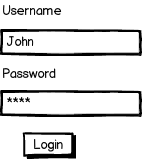
\includegraphics[]{../img/mockups/login.png}
  }
  \end{center}
  \caption{Okno logowania}
  \label{fig:mockups-login}
\end{figure}

\begin{figure}[H]
  \begin{center}
  \fbox{
    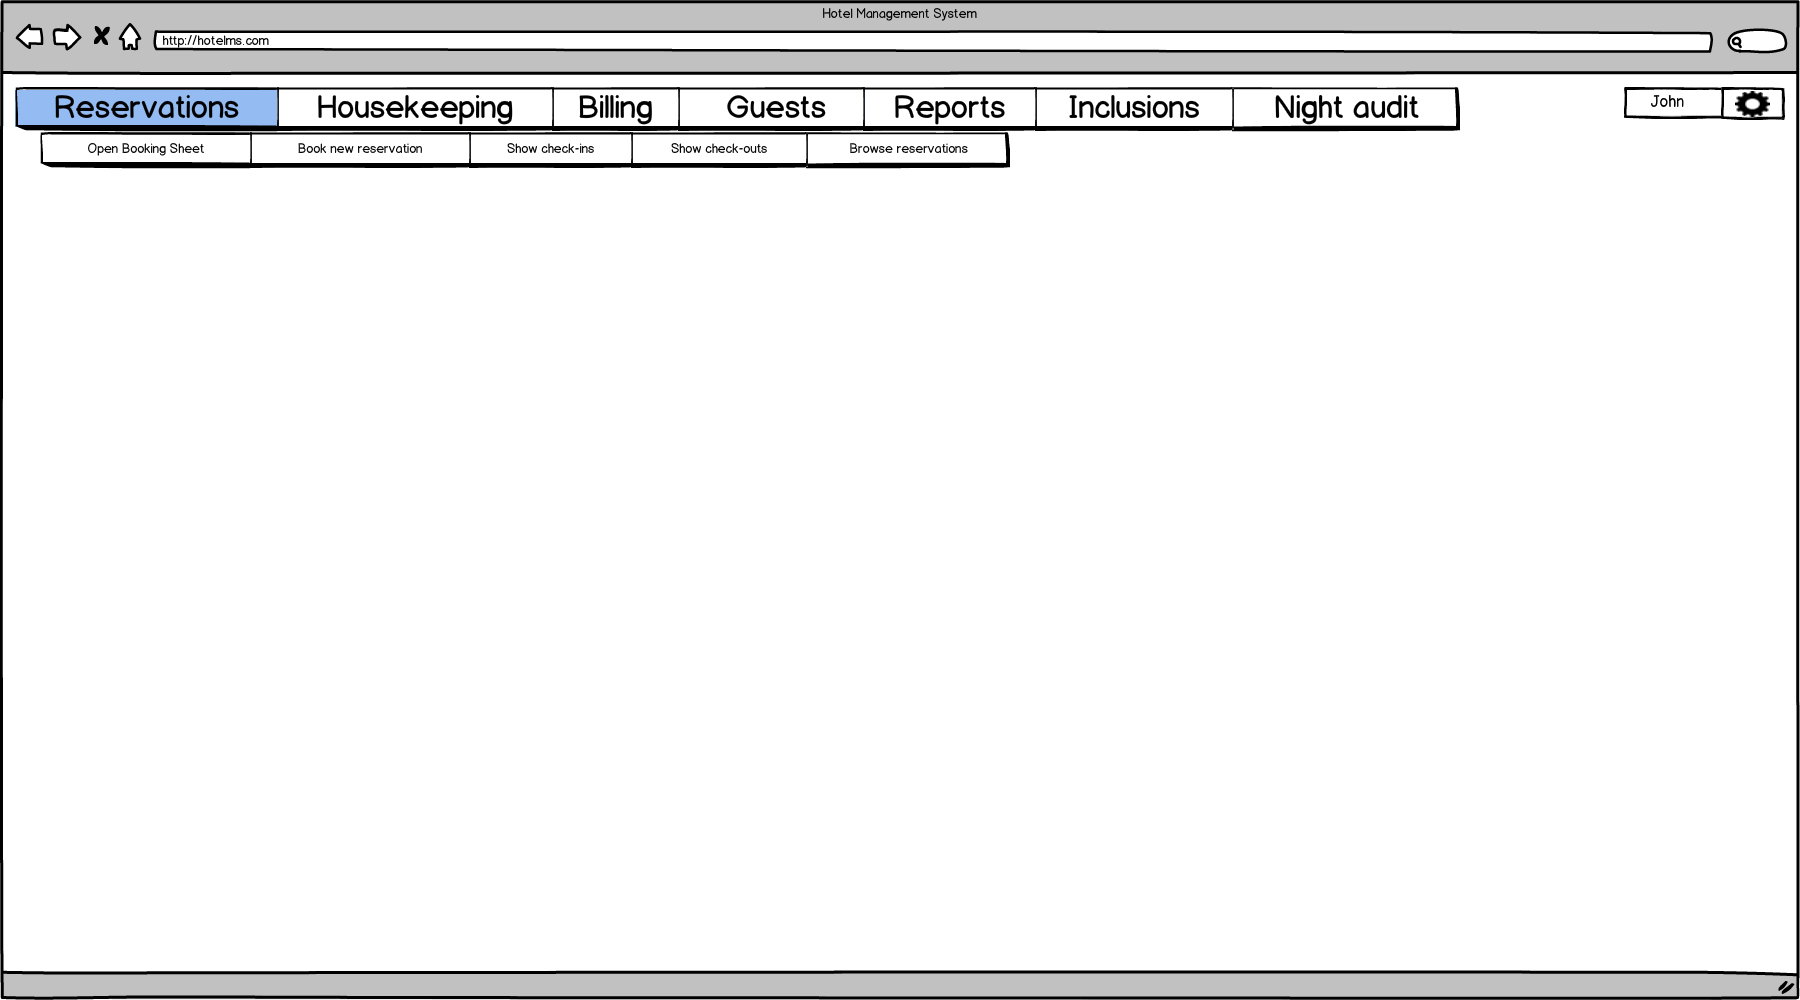
\includegraphics[scale=0.35, angle=270]{../img/mockups/reservations-module-selected-v3.png}
  }
  \end{center}
  \caption{Główny panel aplikacji z włączonym modułem rezerwacyjnym}
  \label{fig:mockups-main-panel}
\end{figure}

\begin{figure}[H]
  \begin{center}
  \fbox{
    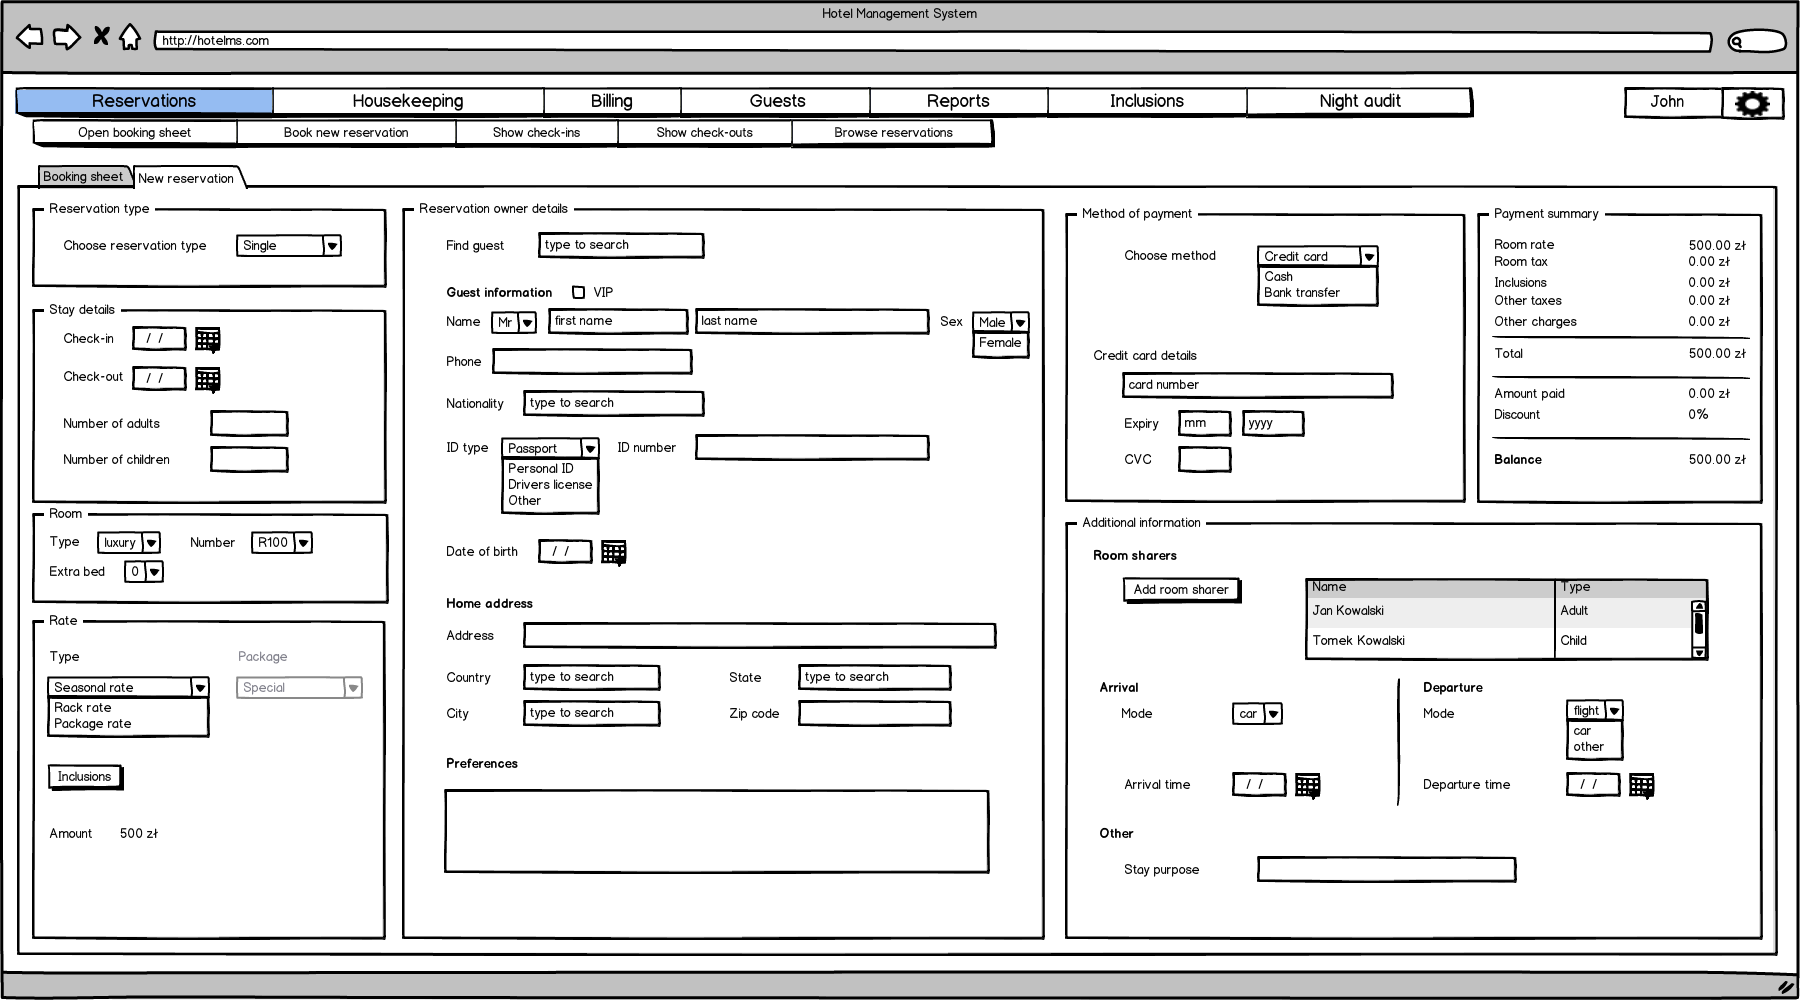
\includegraphics[scale=0.35, angle=270]{../img/mockups/book-new-reservation.png}
  }
  \end{center}
  \caption{Formularz nowej rezerwacji}
  \label{fig:mockups-new-reservation}
\end{figure}

\begin{figure}[H]
  \begin{center}
  \fbox{
    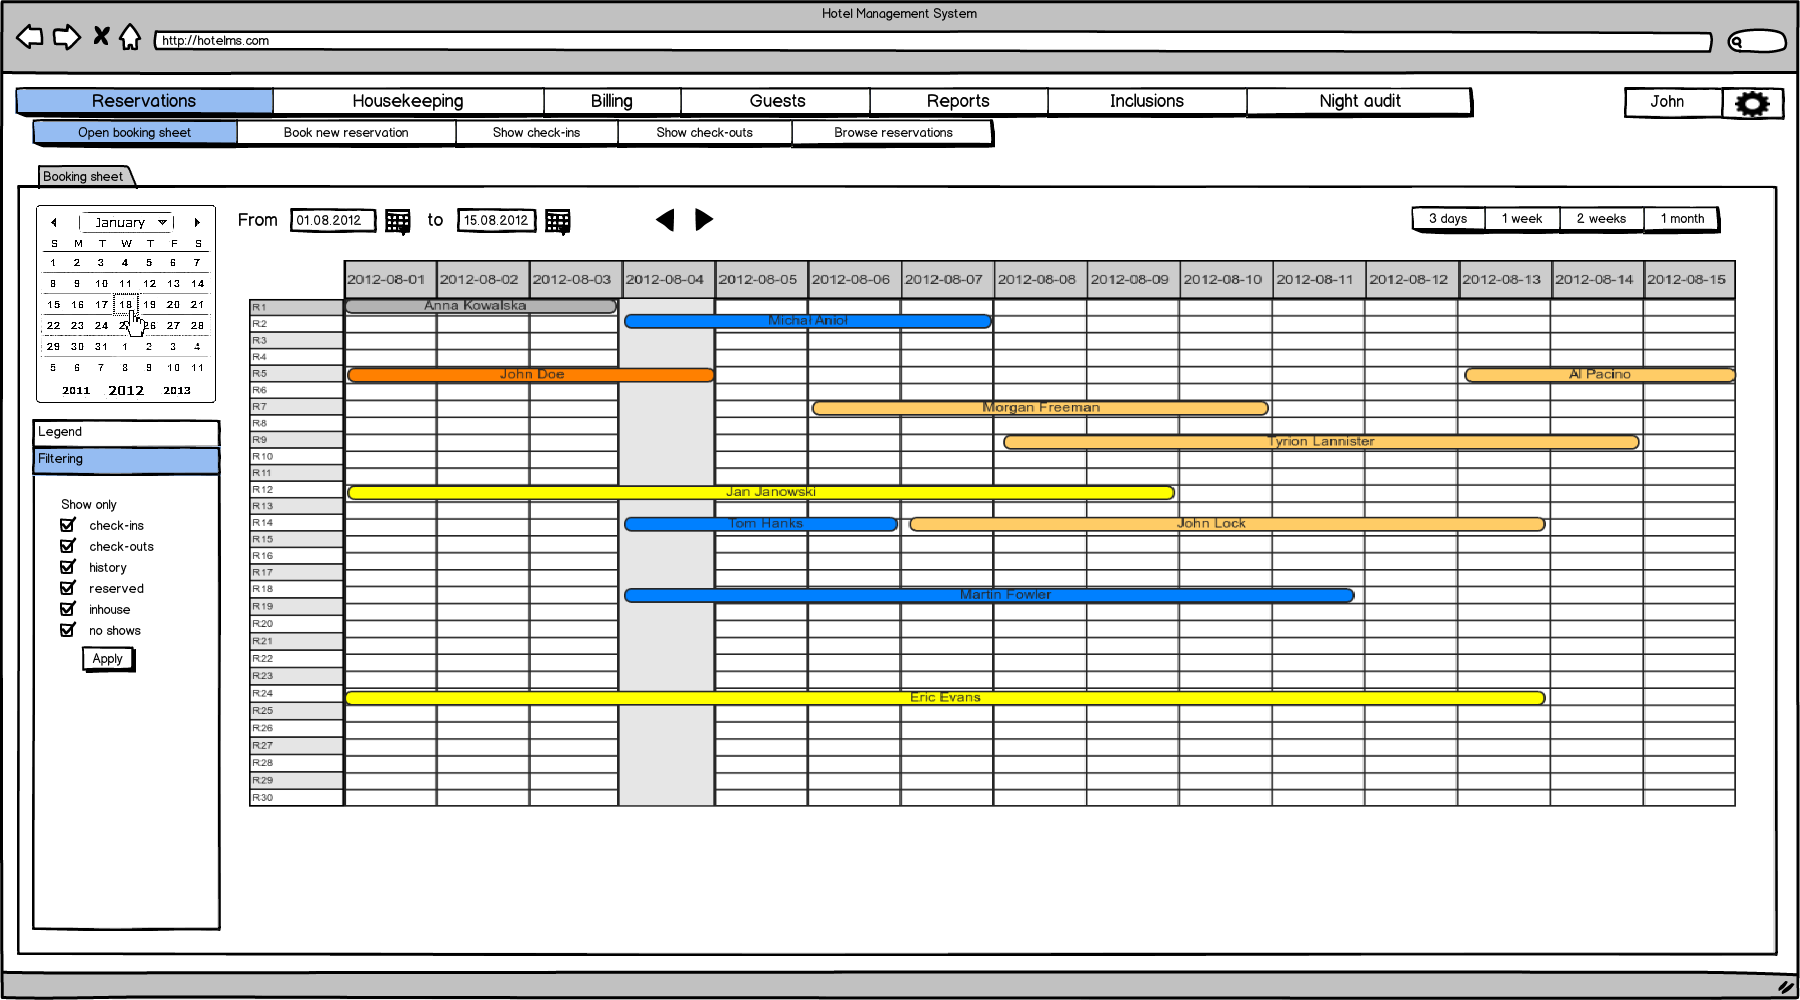
\includegraphics[scale=0.35, angle=270]{../img/mockups/booking-sheet-v3.png}
  }
  \end{center}
  \caption{Ekran z podglągem obłożenia hotelu}
  \label{fig:mockups-booking-sheet}
\end{figure}

\begin{figure}[H]
  \begin{center}
  \fbox{
    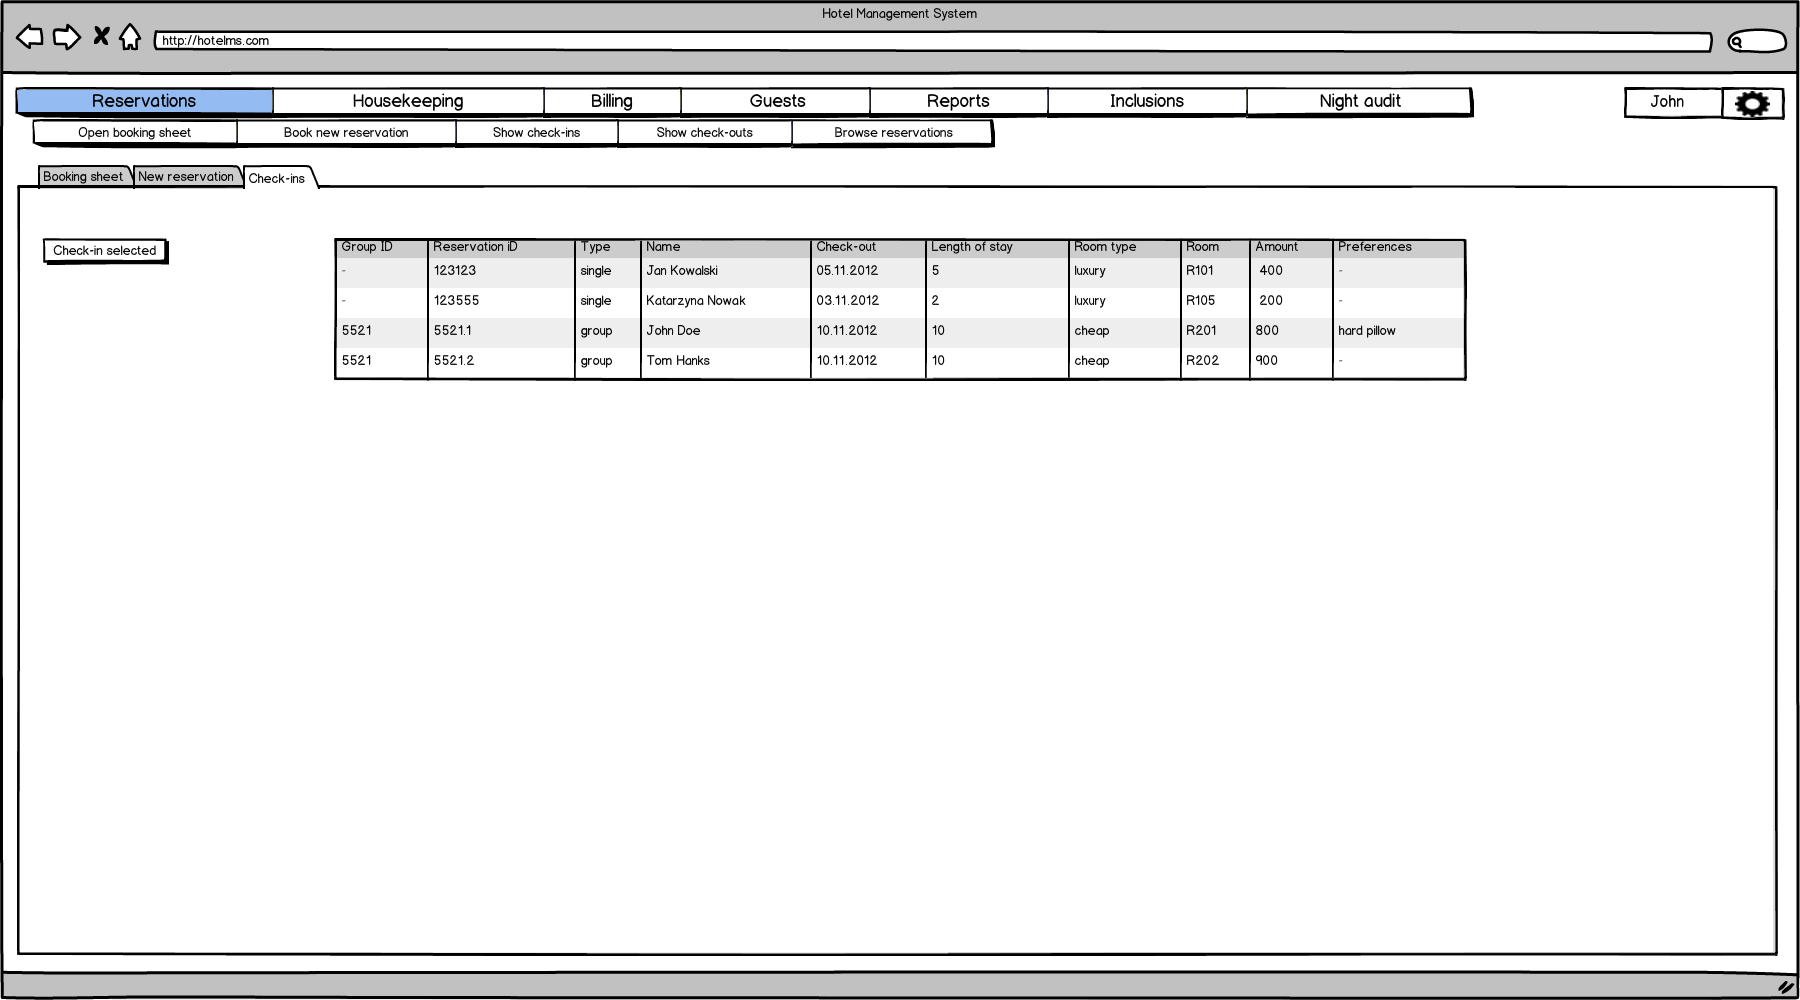
\includegraphics[scale=0.35, angle=270]{../img/mockups/check-ins.png}
  }
  \end{center}
  \caption{Ekran z przyjeżdżającymi dzisiaj gośćmi}
  \label{fig:mockups-checkins}
\end{figure}

\begin{figure}[H]
  \begin{center}
  \fbox{
    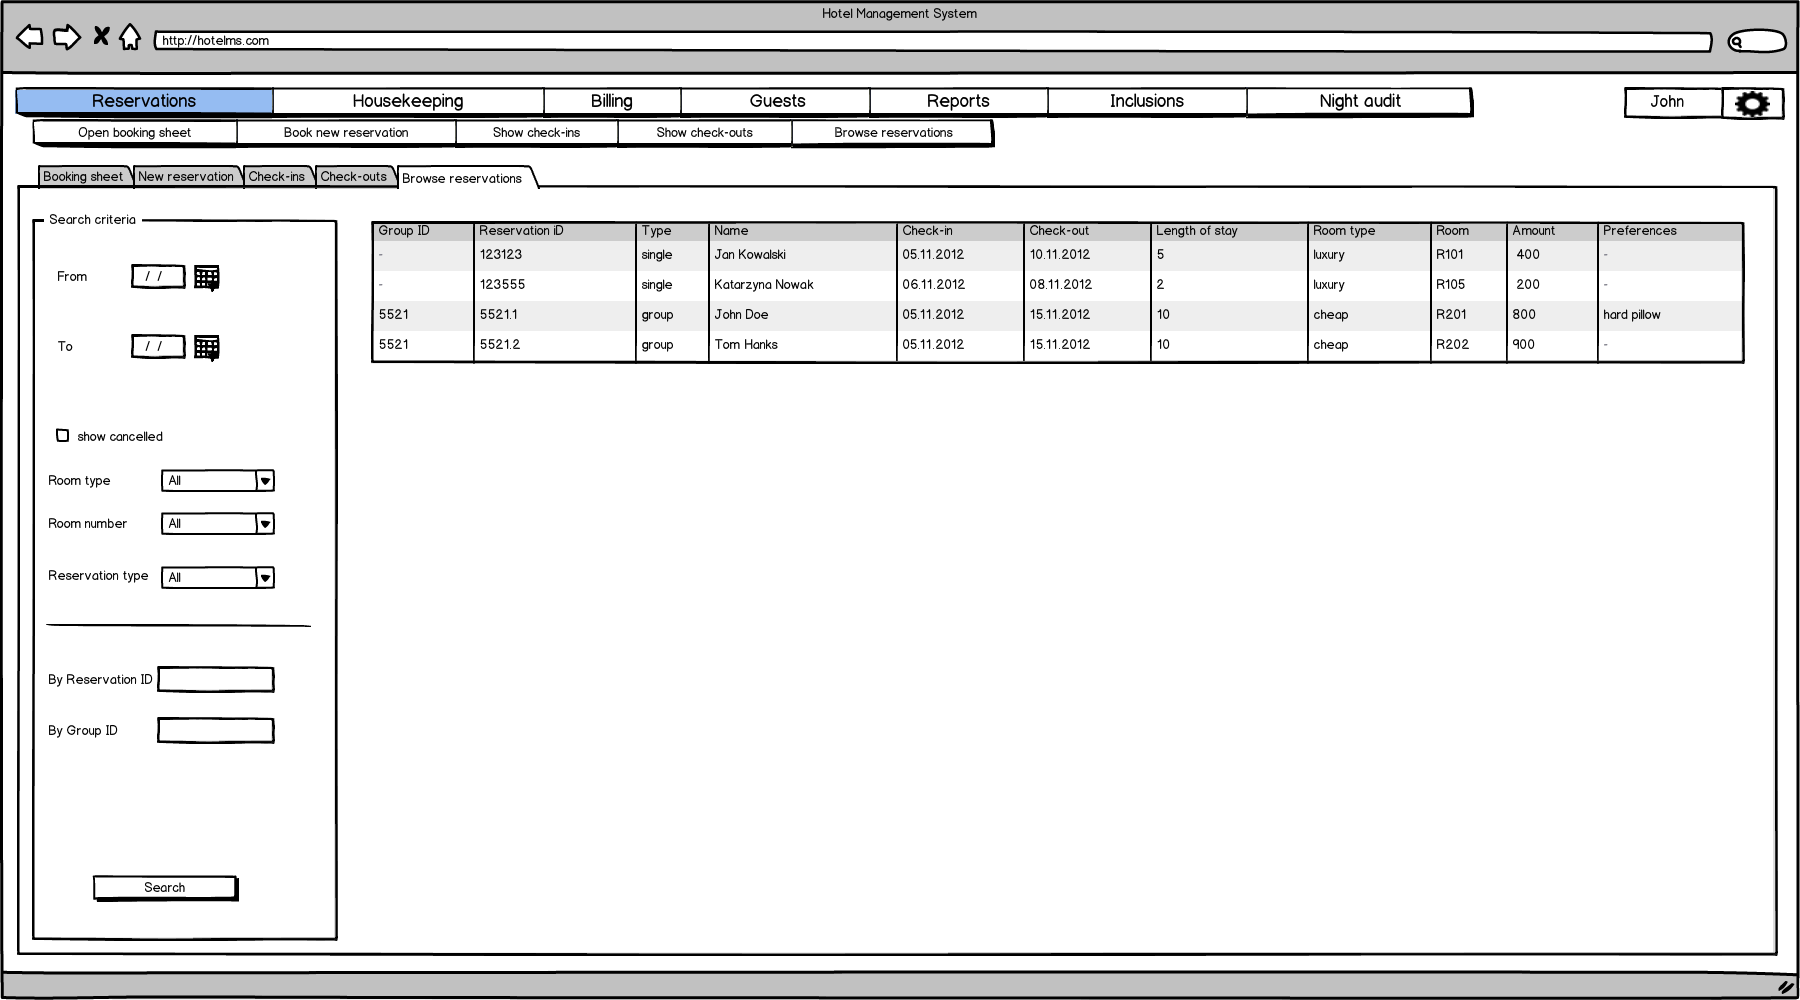
\includegraphics[scale=0.35, angle=270]{../img/mockups/browse-reservations.png}
  }
  \end{center}
  \caption{Ekran z przeglądarką rezerwacji}
  \label{fig:mockups-browse-reservations}
\end{figure}



\chapter{Wygląd aplikacji}


\begin{figure}[H]
  \begin{center}
  \fbox{
    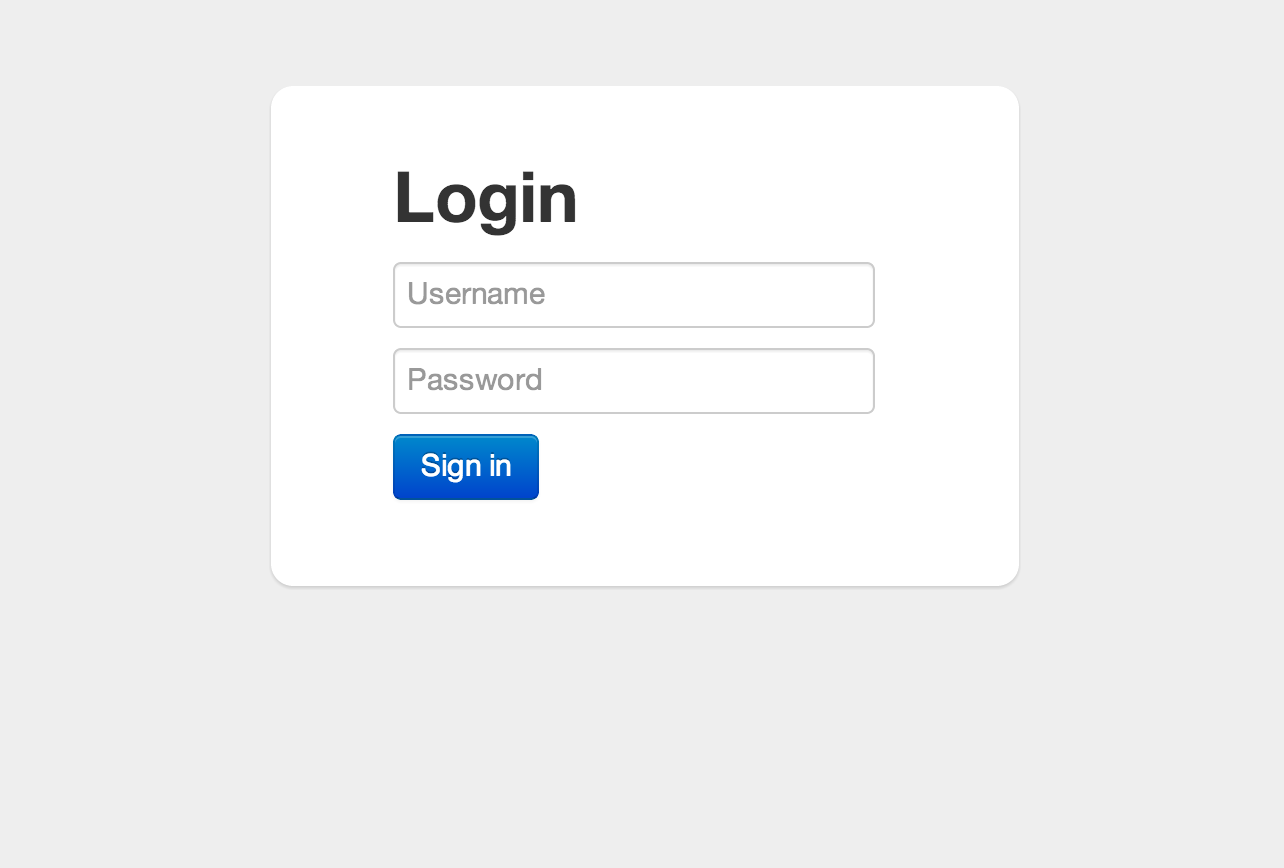
\includegraphics[scale=0.3, angle=270]{../img/wyglad/login-form.png}
  }
  \end{center}
  \caption{Ekran logowania}
  \label{fig:app-login-form}
\end{figure}

\begin{figure}[H]
  \begin{center}
  \fbox{
    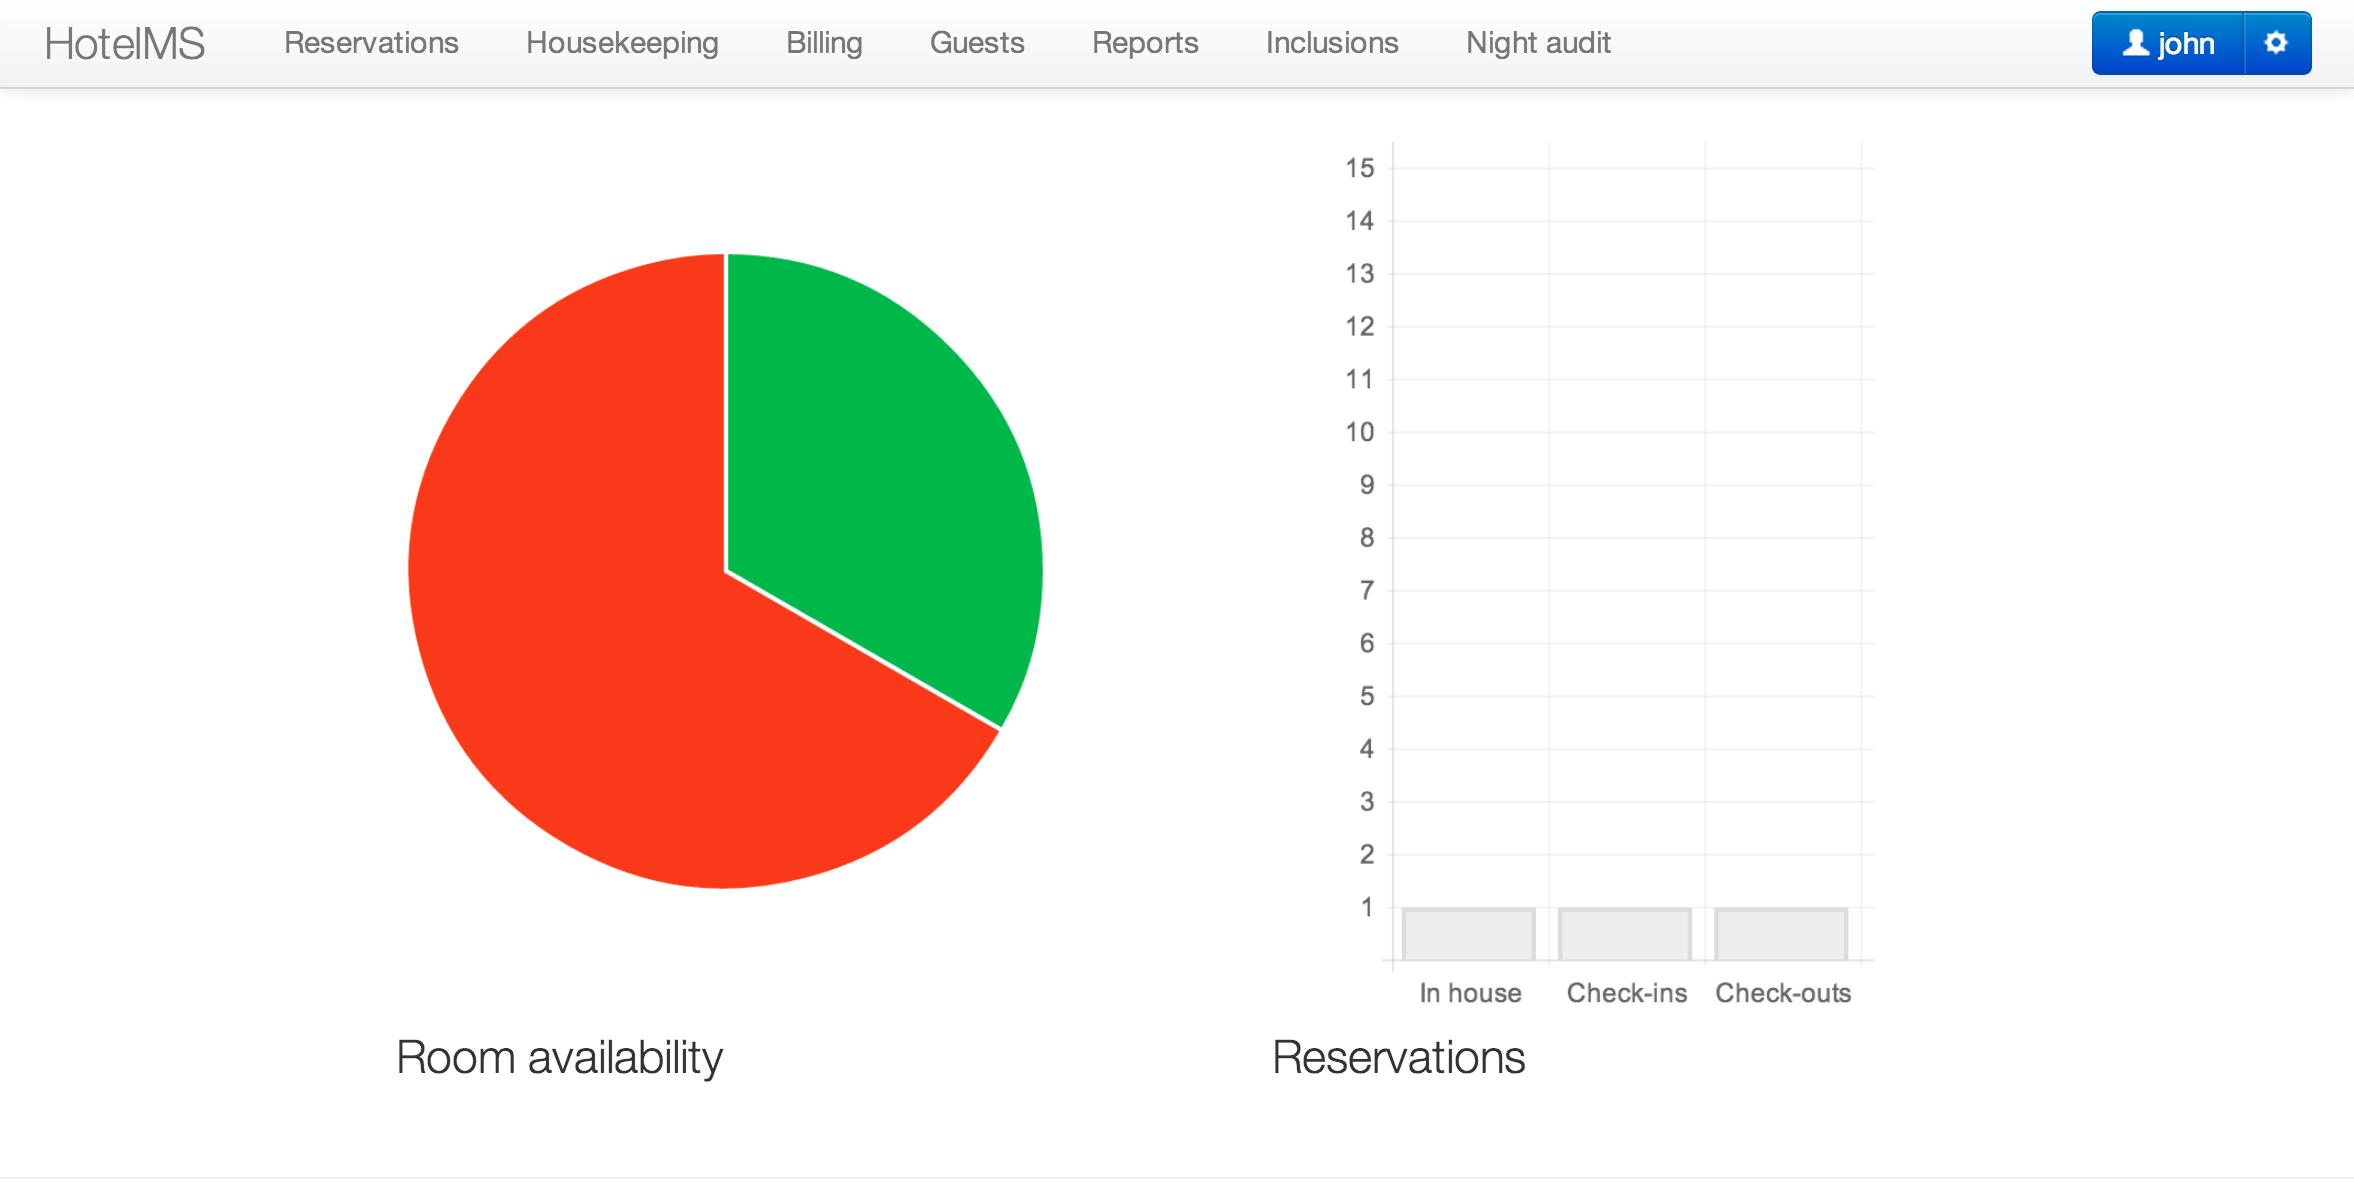
\includegraphics[scale=0.25, angle=270]{../img/wyglad/dashboard.png}
  }
  \end{center}
  \caption{Dashboard aplikacji ze statystykami}
  \label{fig:app-dashboard}
\end{figure}

\begin{figure}[H]
  \begin{center}
  \fbox{
    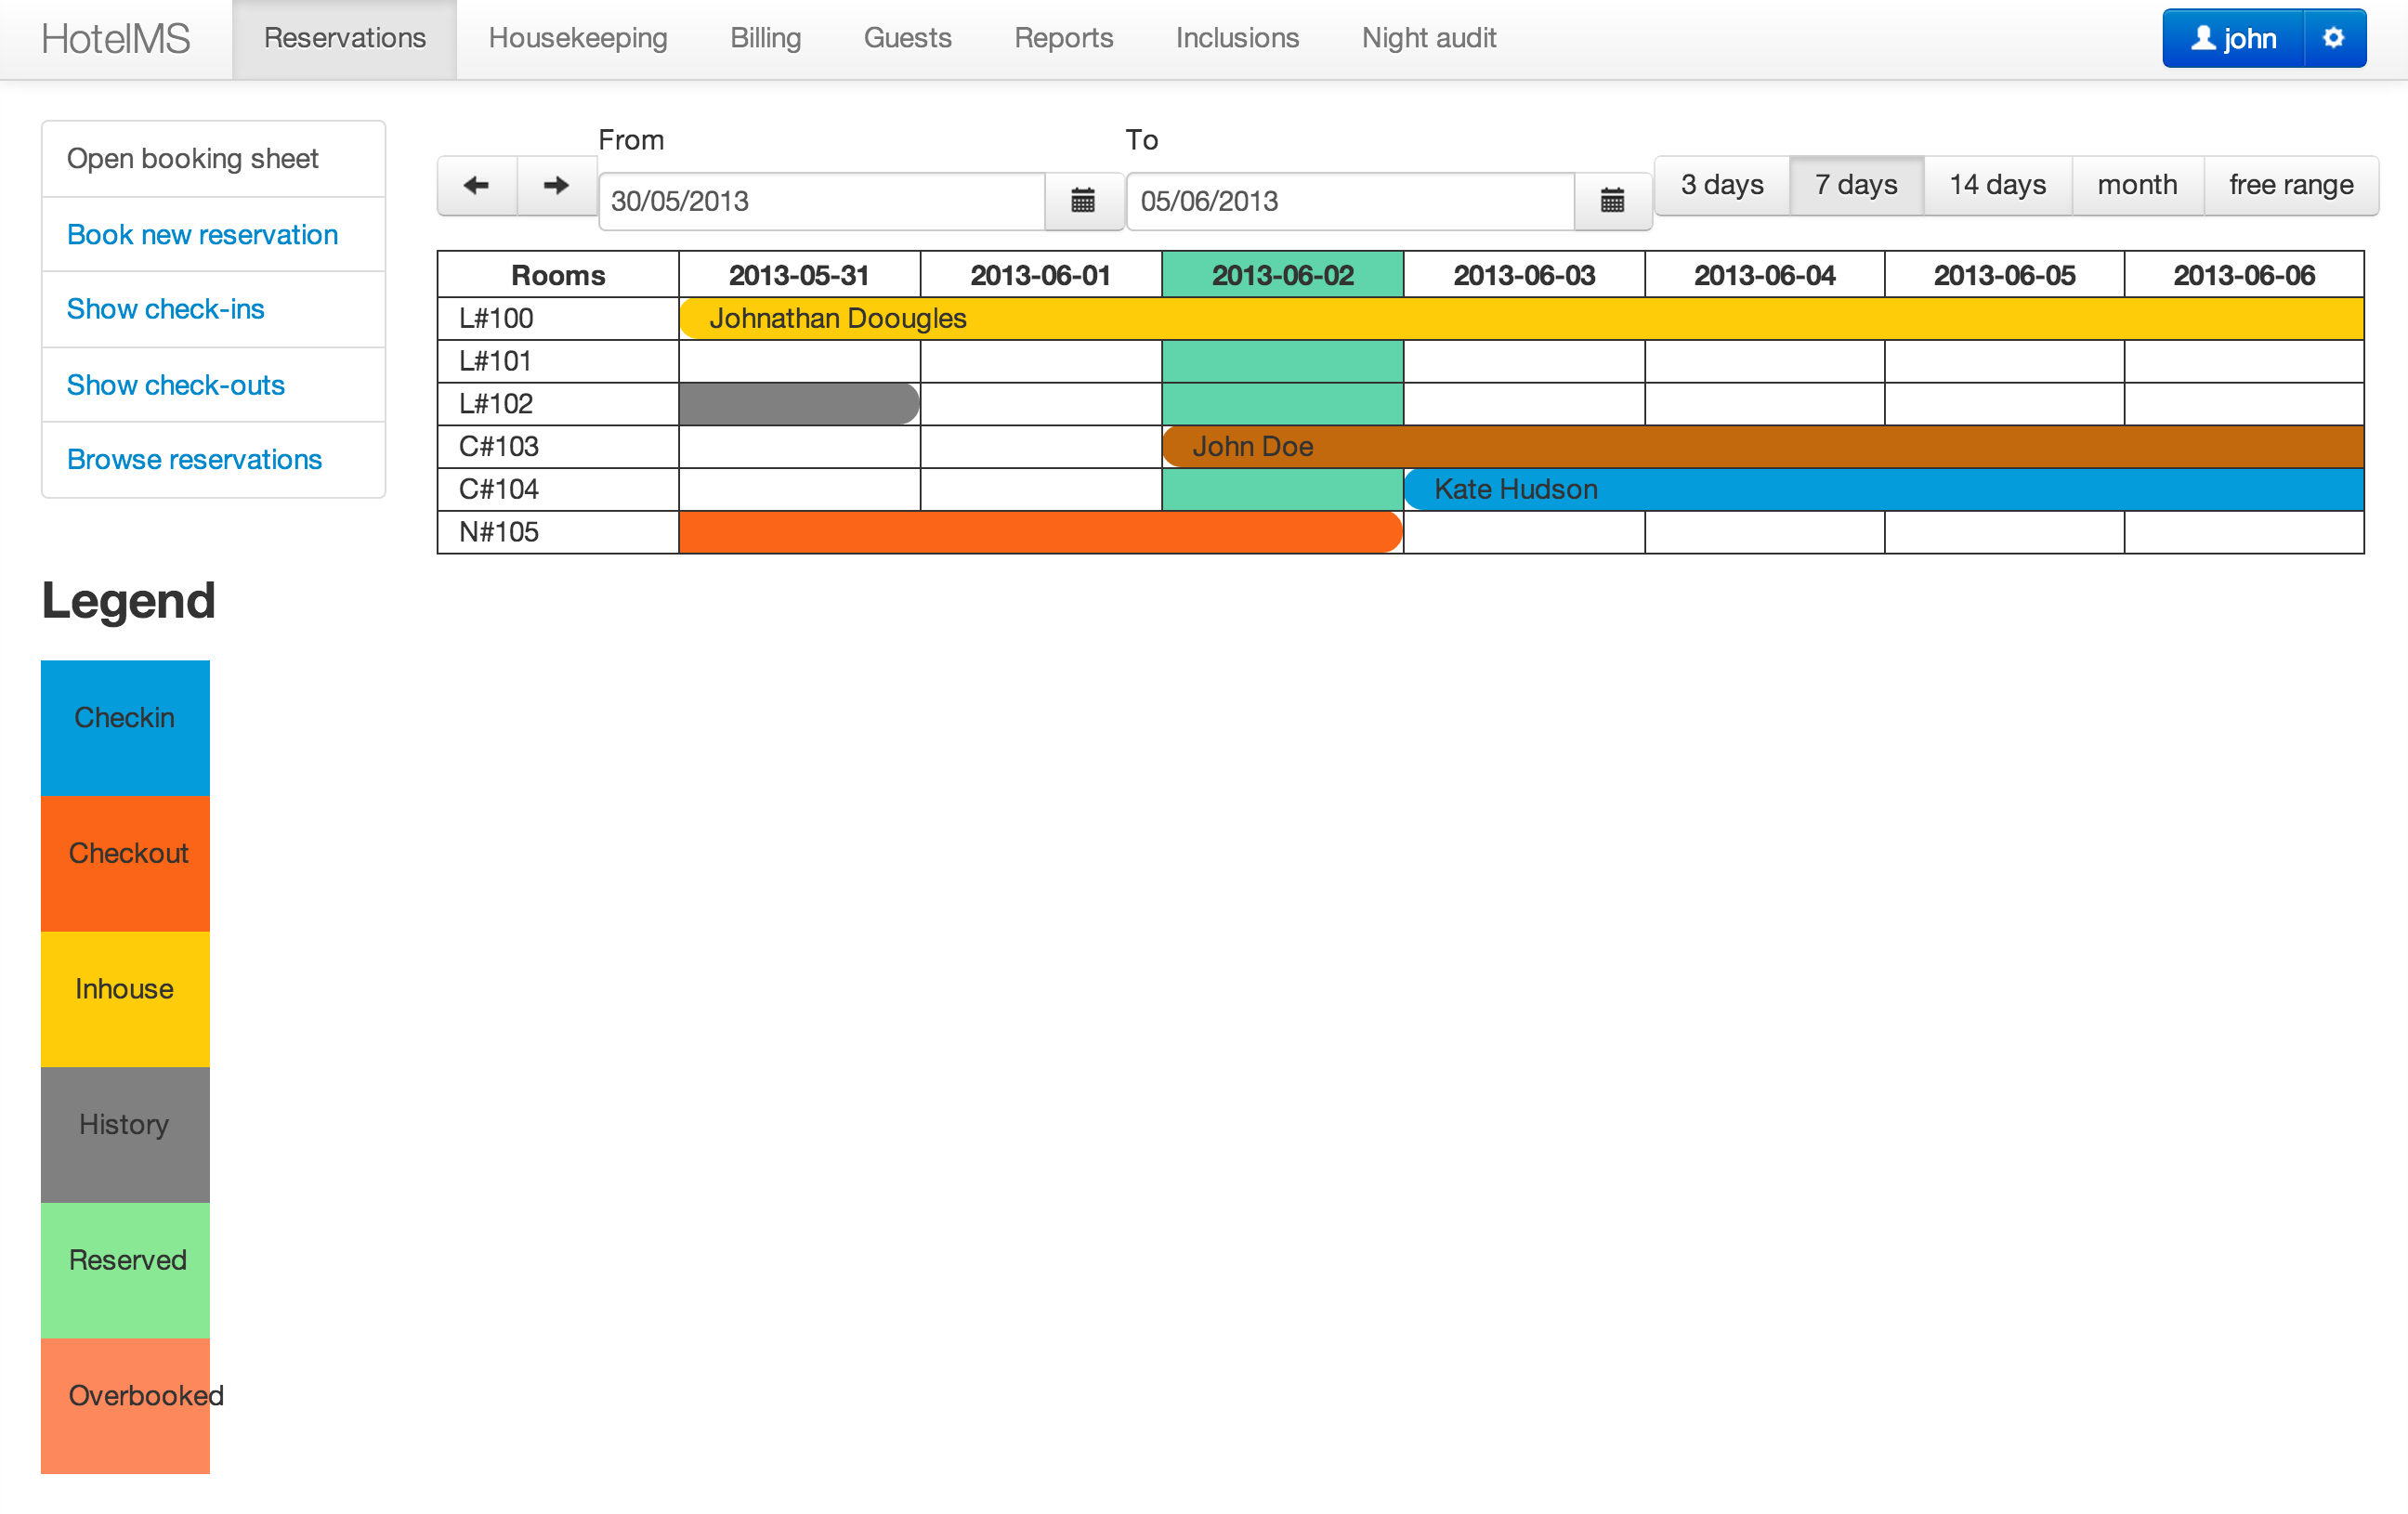
\includegraphics[scale=0.25, angle=270]{../img/wyglad/booking-sheet.png}
  }
  \end{center}
  \caption{Podgląd obłożenia hotelu}
  \label{fig:app-booking-sheet}
\end{figure}

\begin{figure}[H]
  \begin{center}
  \fbox{
    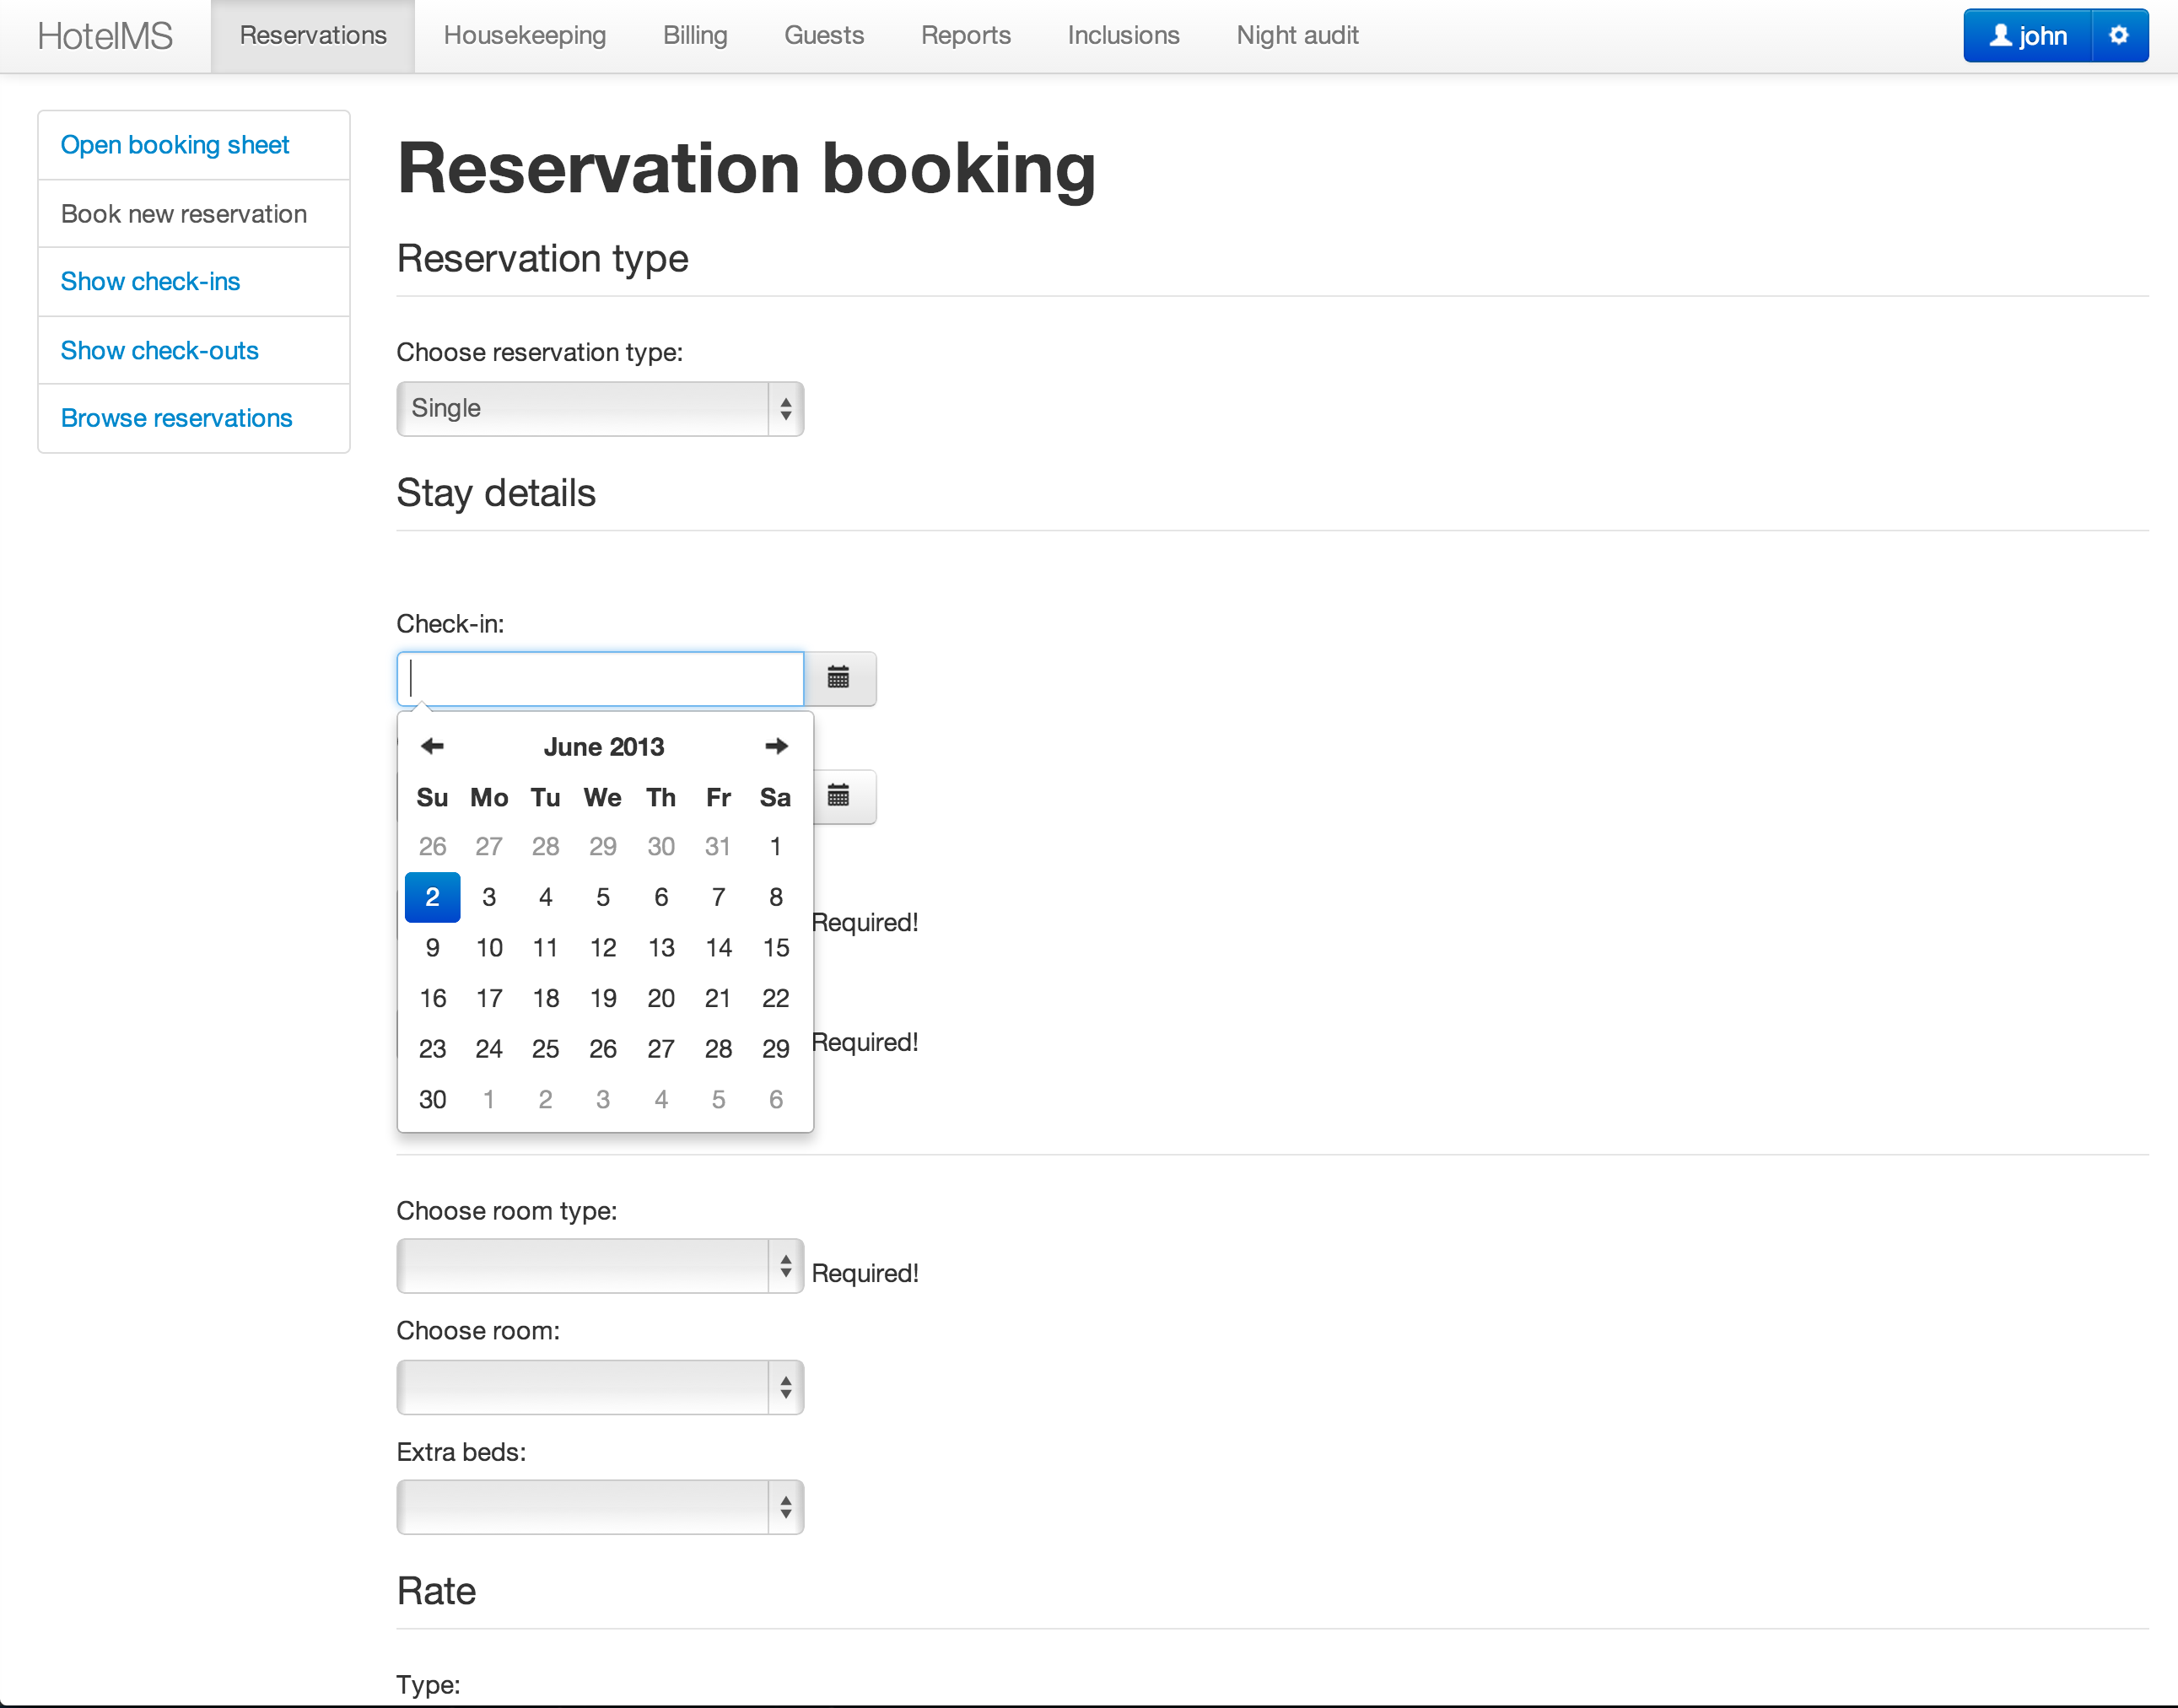
\includegraphics[scale=0.2, angle=270]{../img/wyglad/new-res-p1.png}
  }
  \end{center}
  \caption{Część I formularza nowej rezerwacji}
  \label{fig:app-new-reservation-p1}
\end{figure}

\begin{figure}[H]
  \begin{center}
  \fbox{
    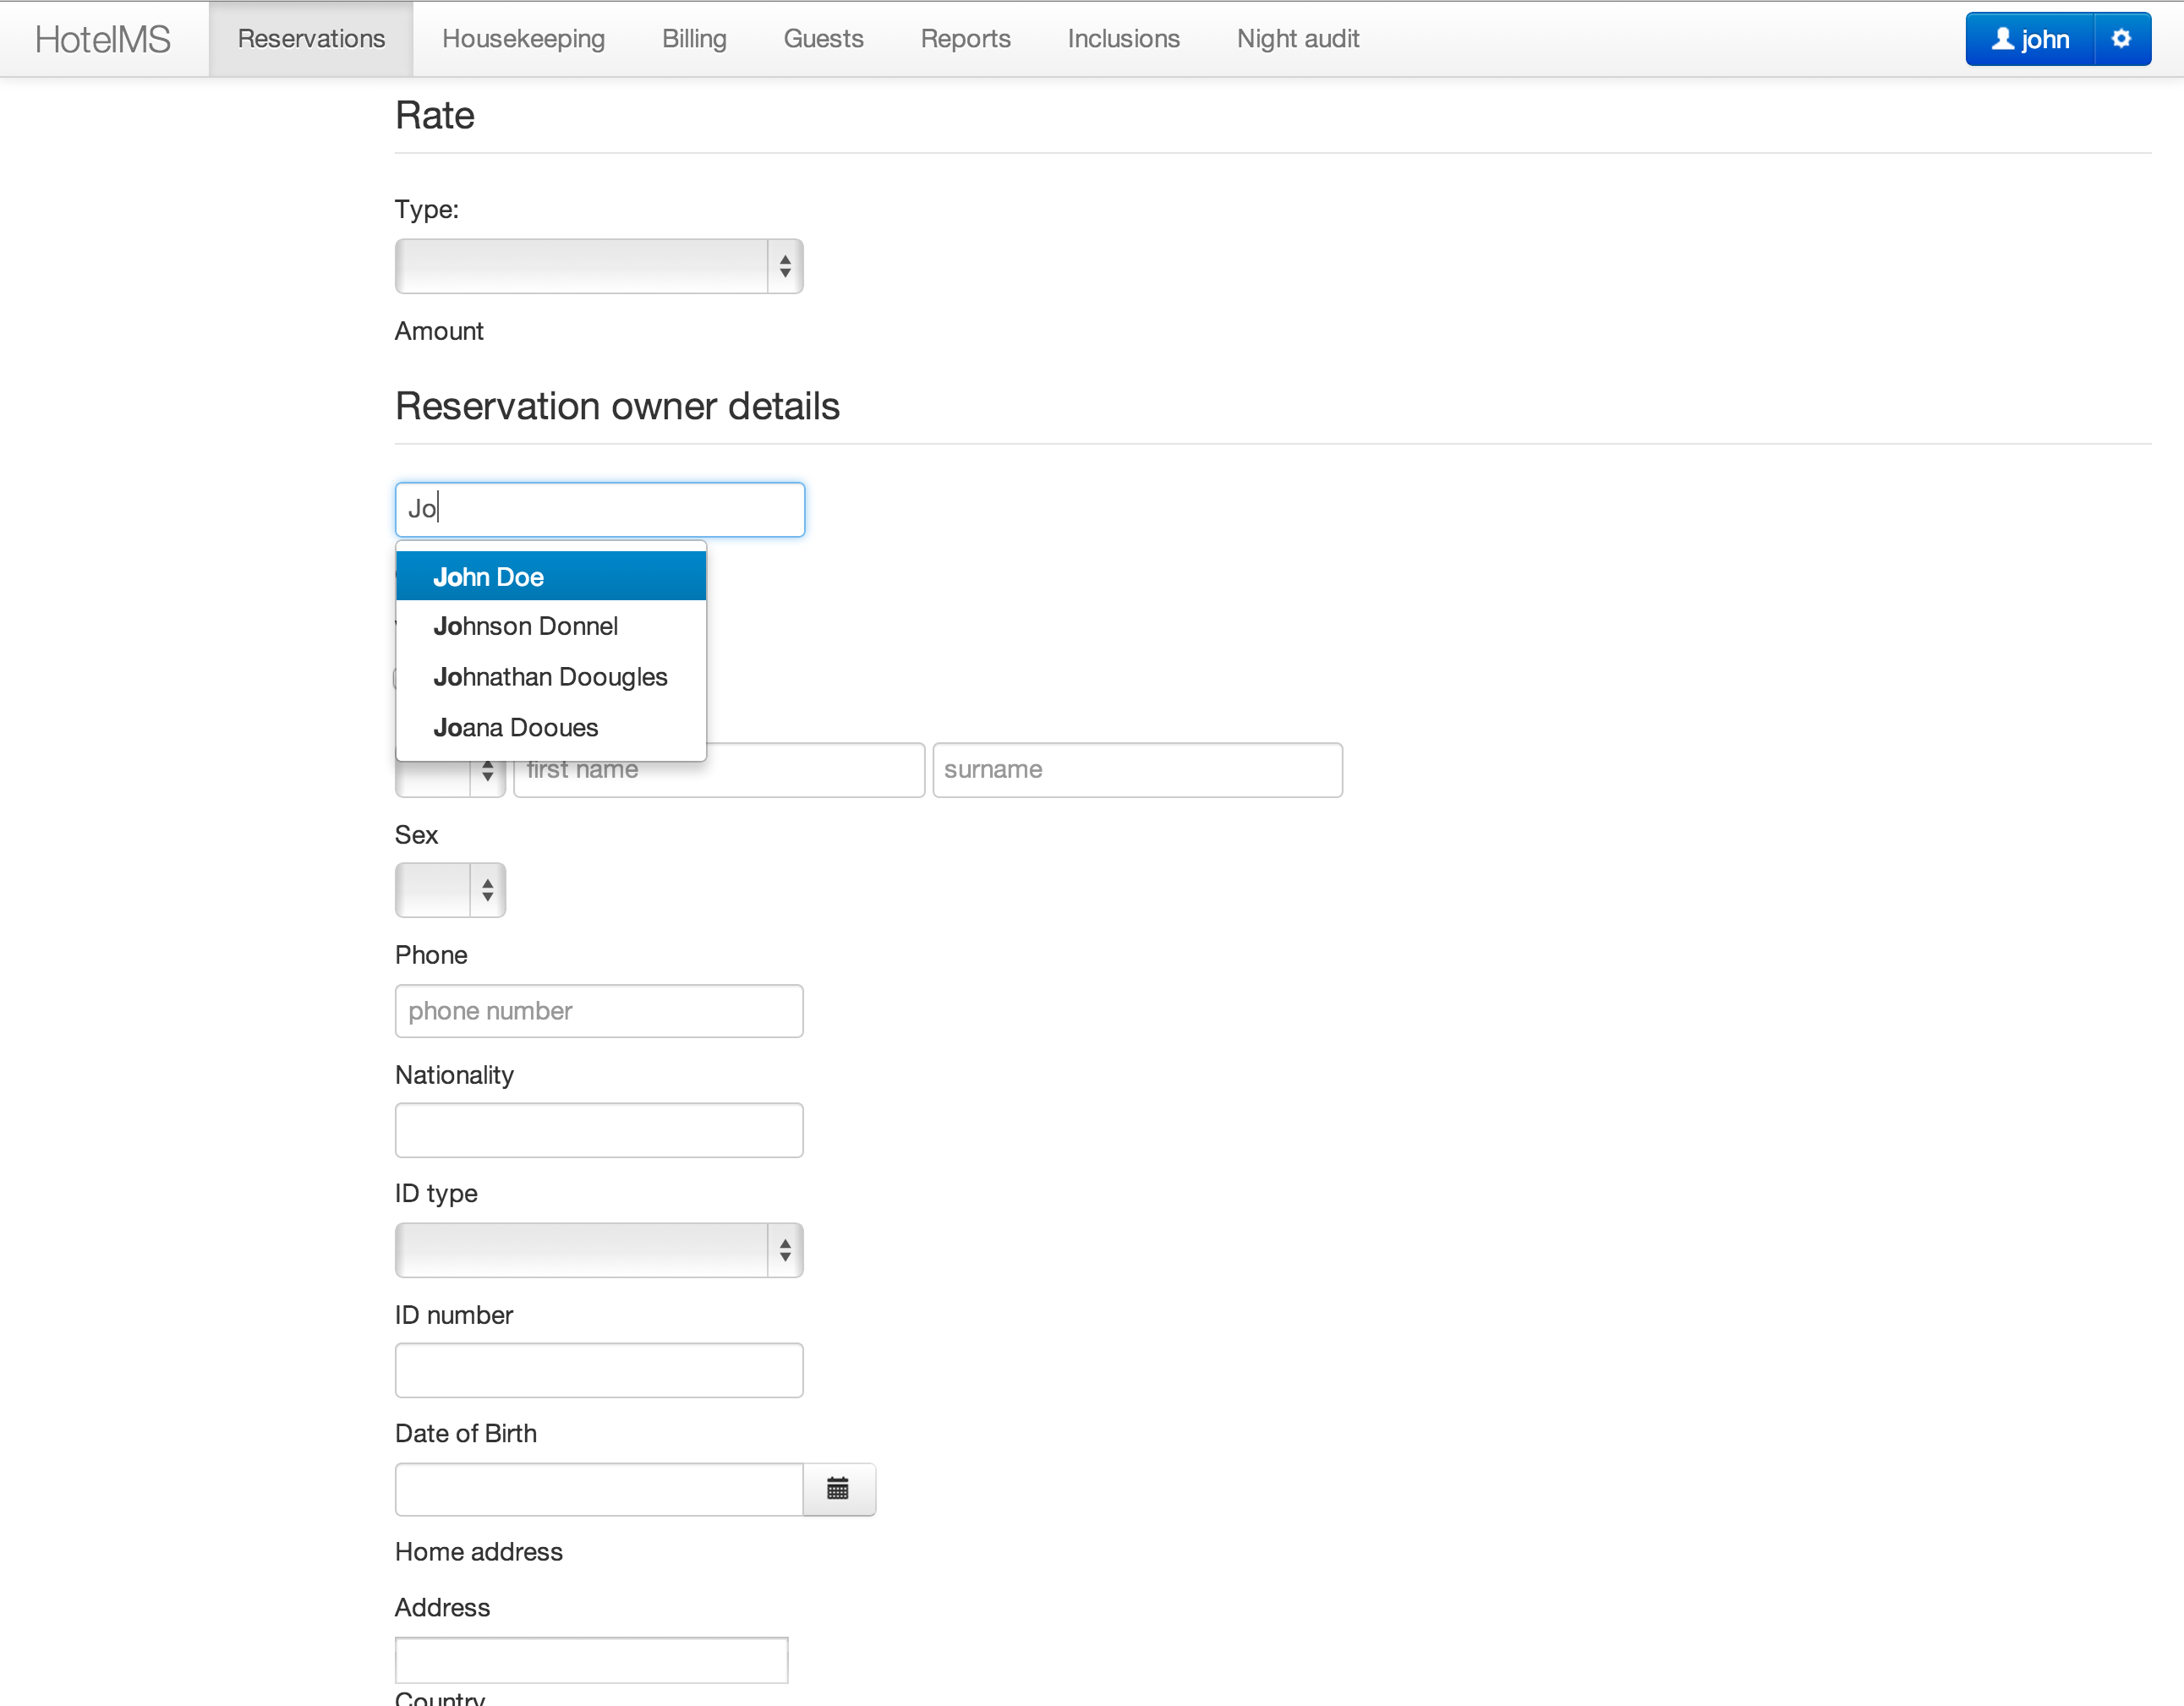
\includegraphics[scale=0.2, angle=270]{../img/wyglad/new-res-p2.png}
  }
  \end{center}
  \caption{Część II formularza nowej rezerwacji}
  \label{fig:app-new-reservation-p2}
\end{figure}

\begin{figure}[H]
  \begin{center}
  \fbox{
    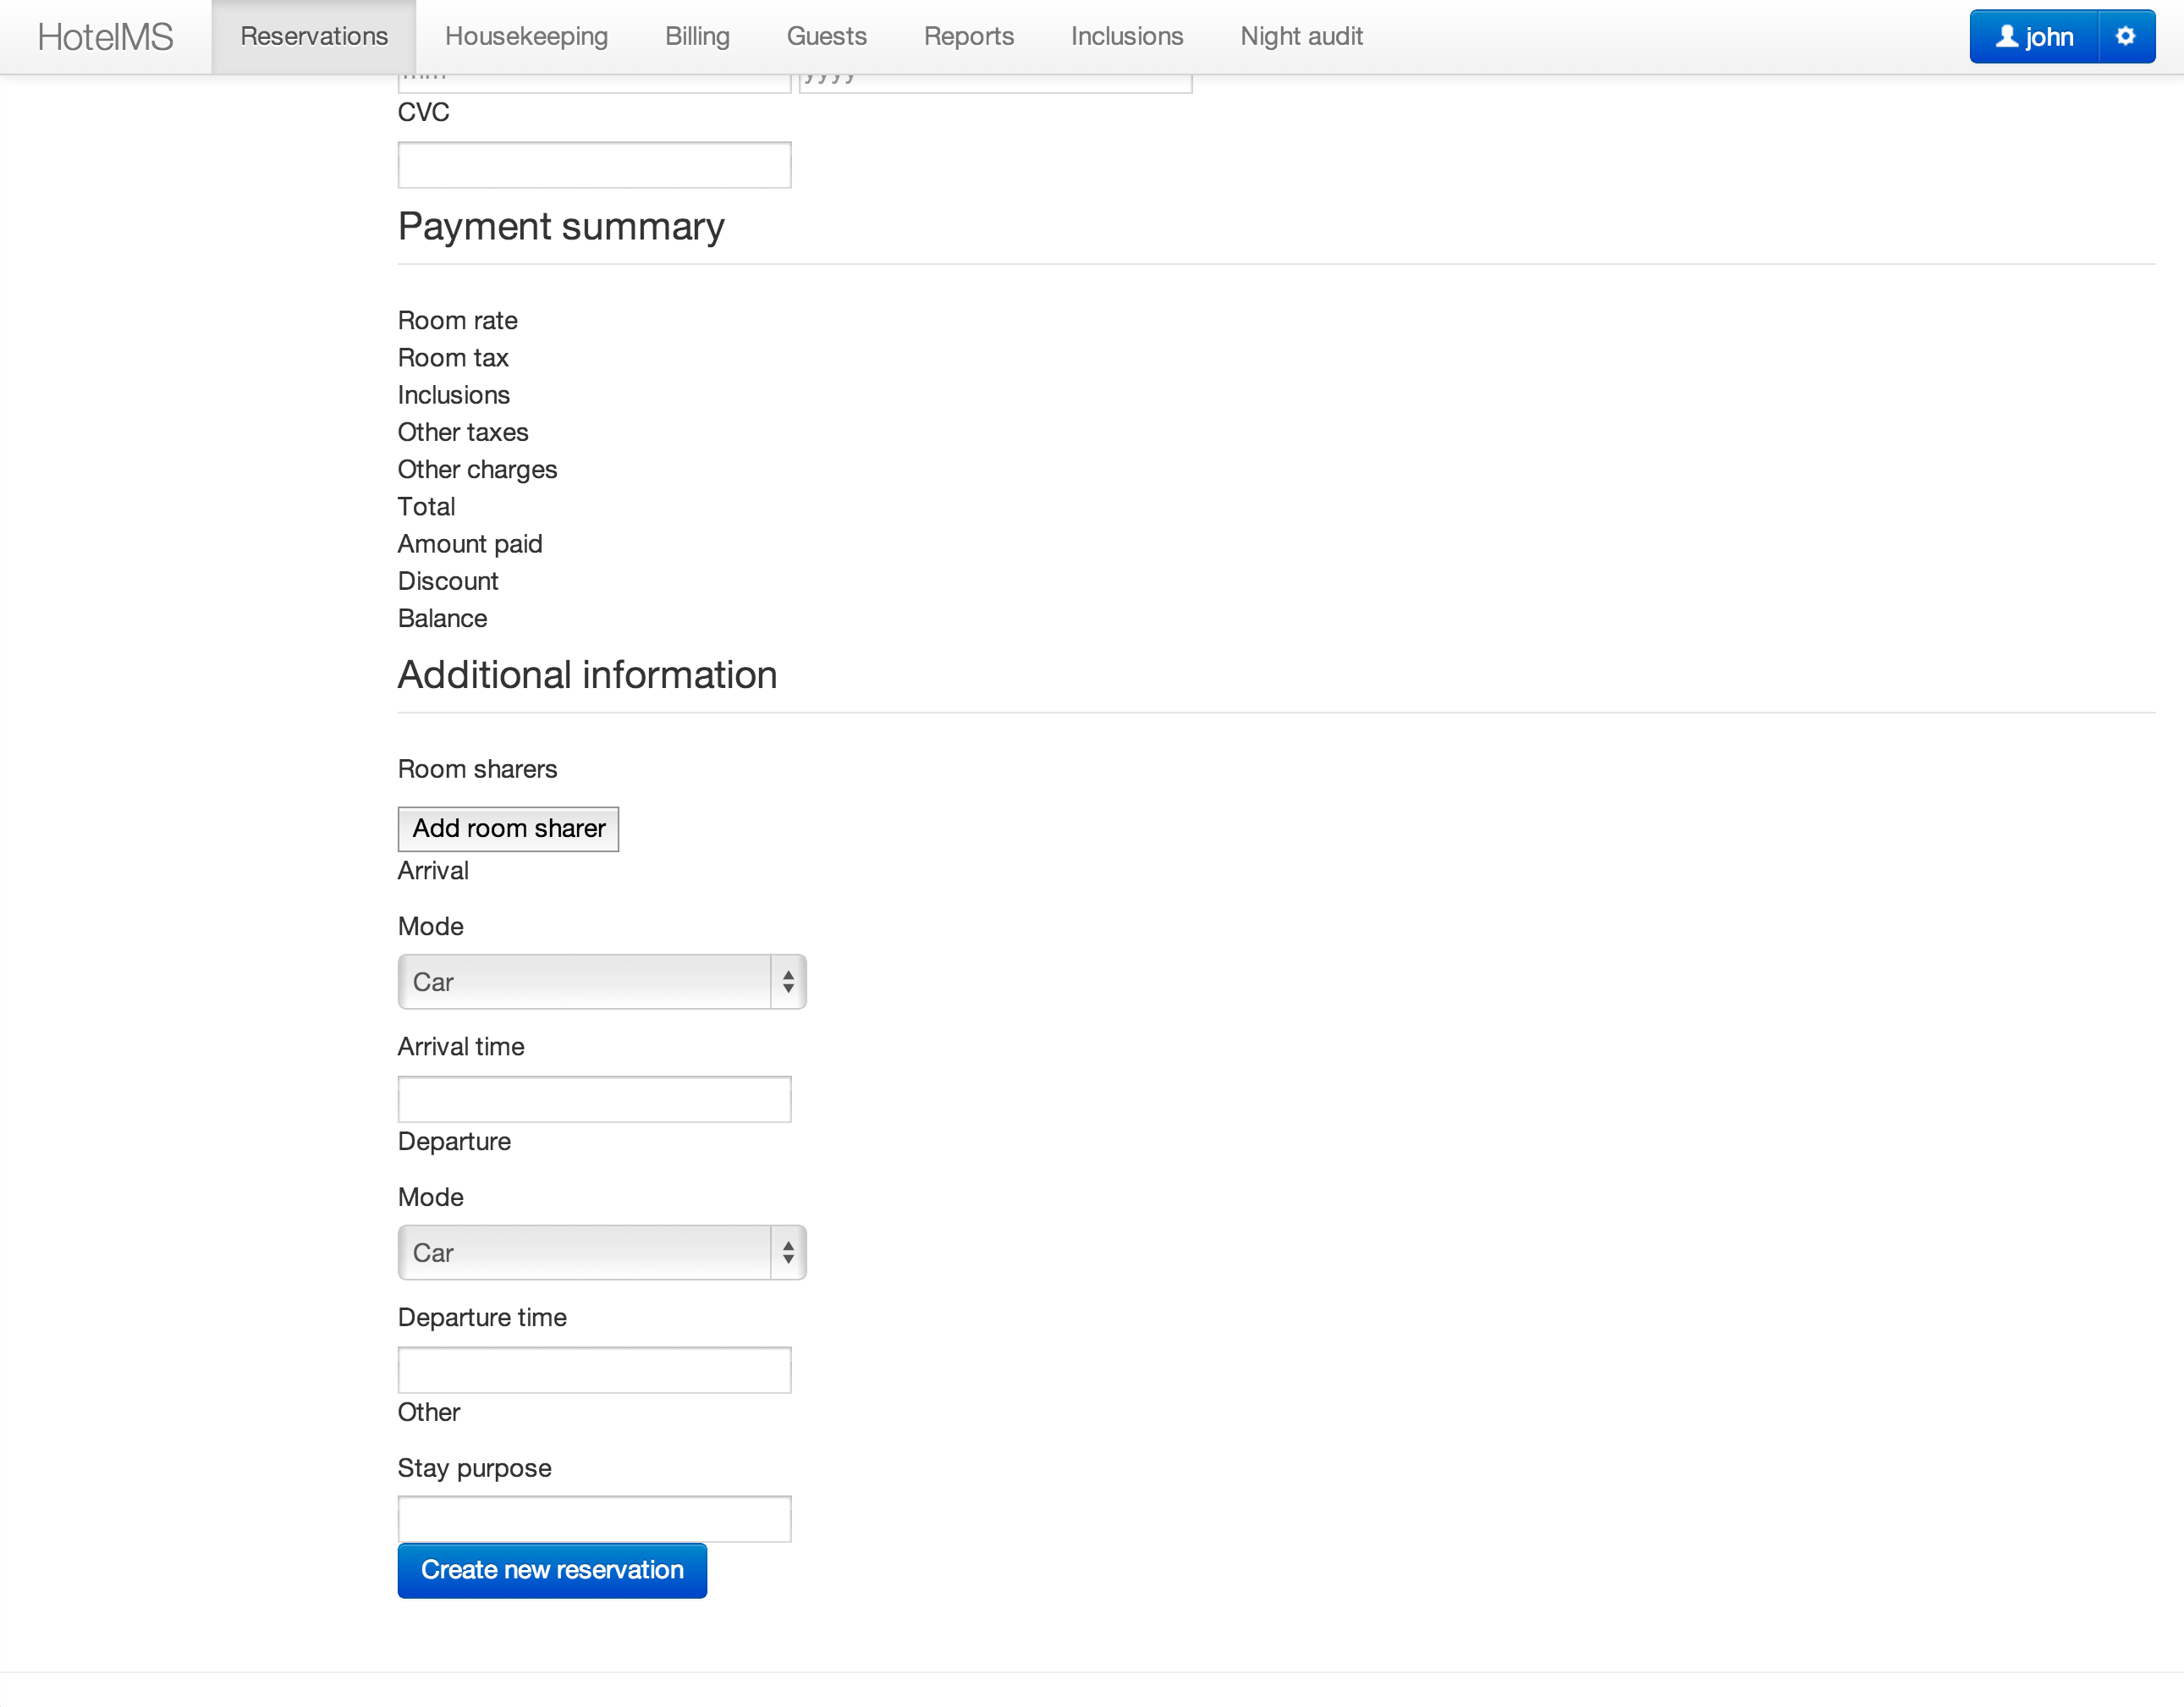
\includegraphics[scale=0.2, angle=270]{../img/wyglad/new-res-p3.png}
  }
  \end{center}
  \caption{Część III formularza nowej rezerwacji}
  \label{fig:app-new-reservation-p3}
\end{figure}

\begin{figure}[H]
  \begin{center}
  \fbox{
    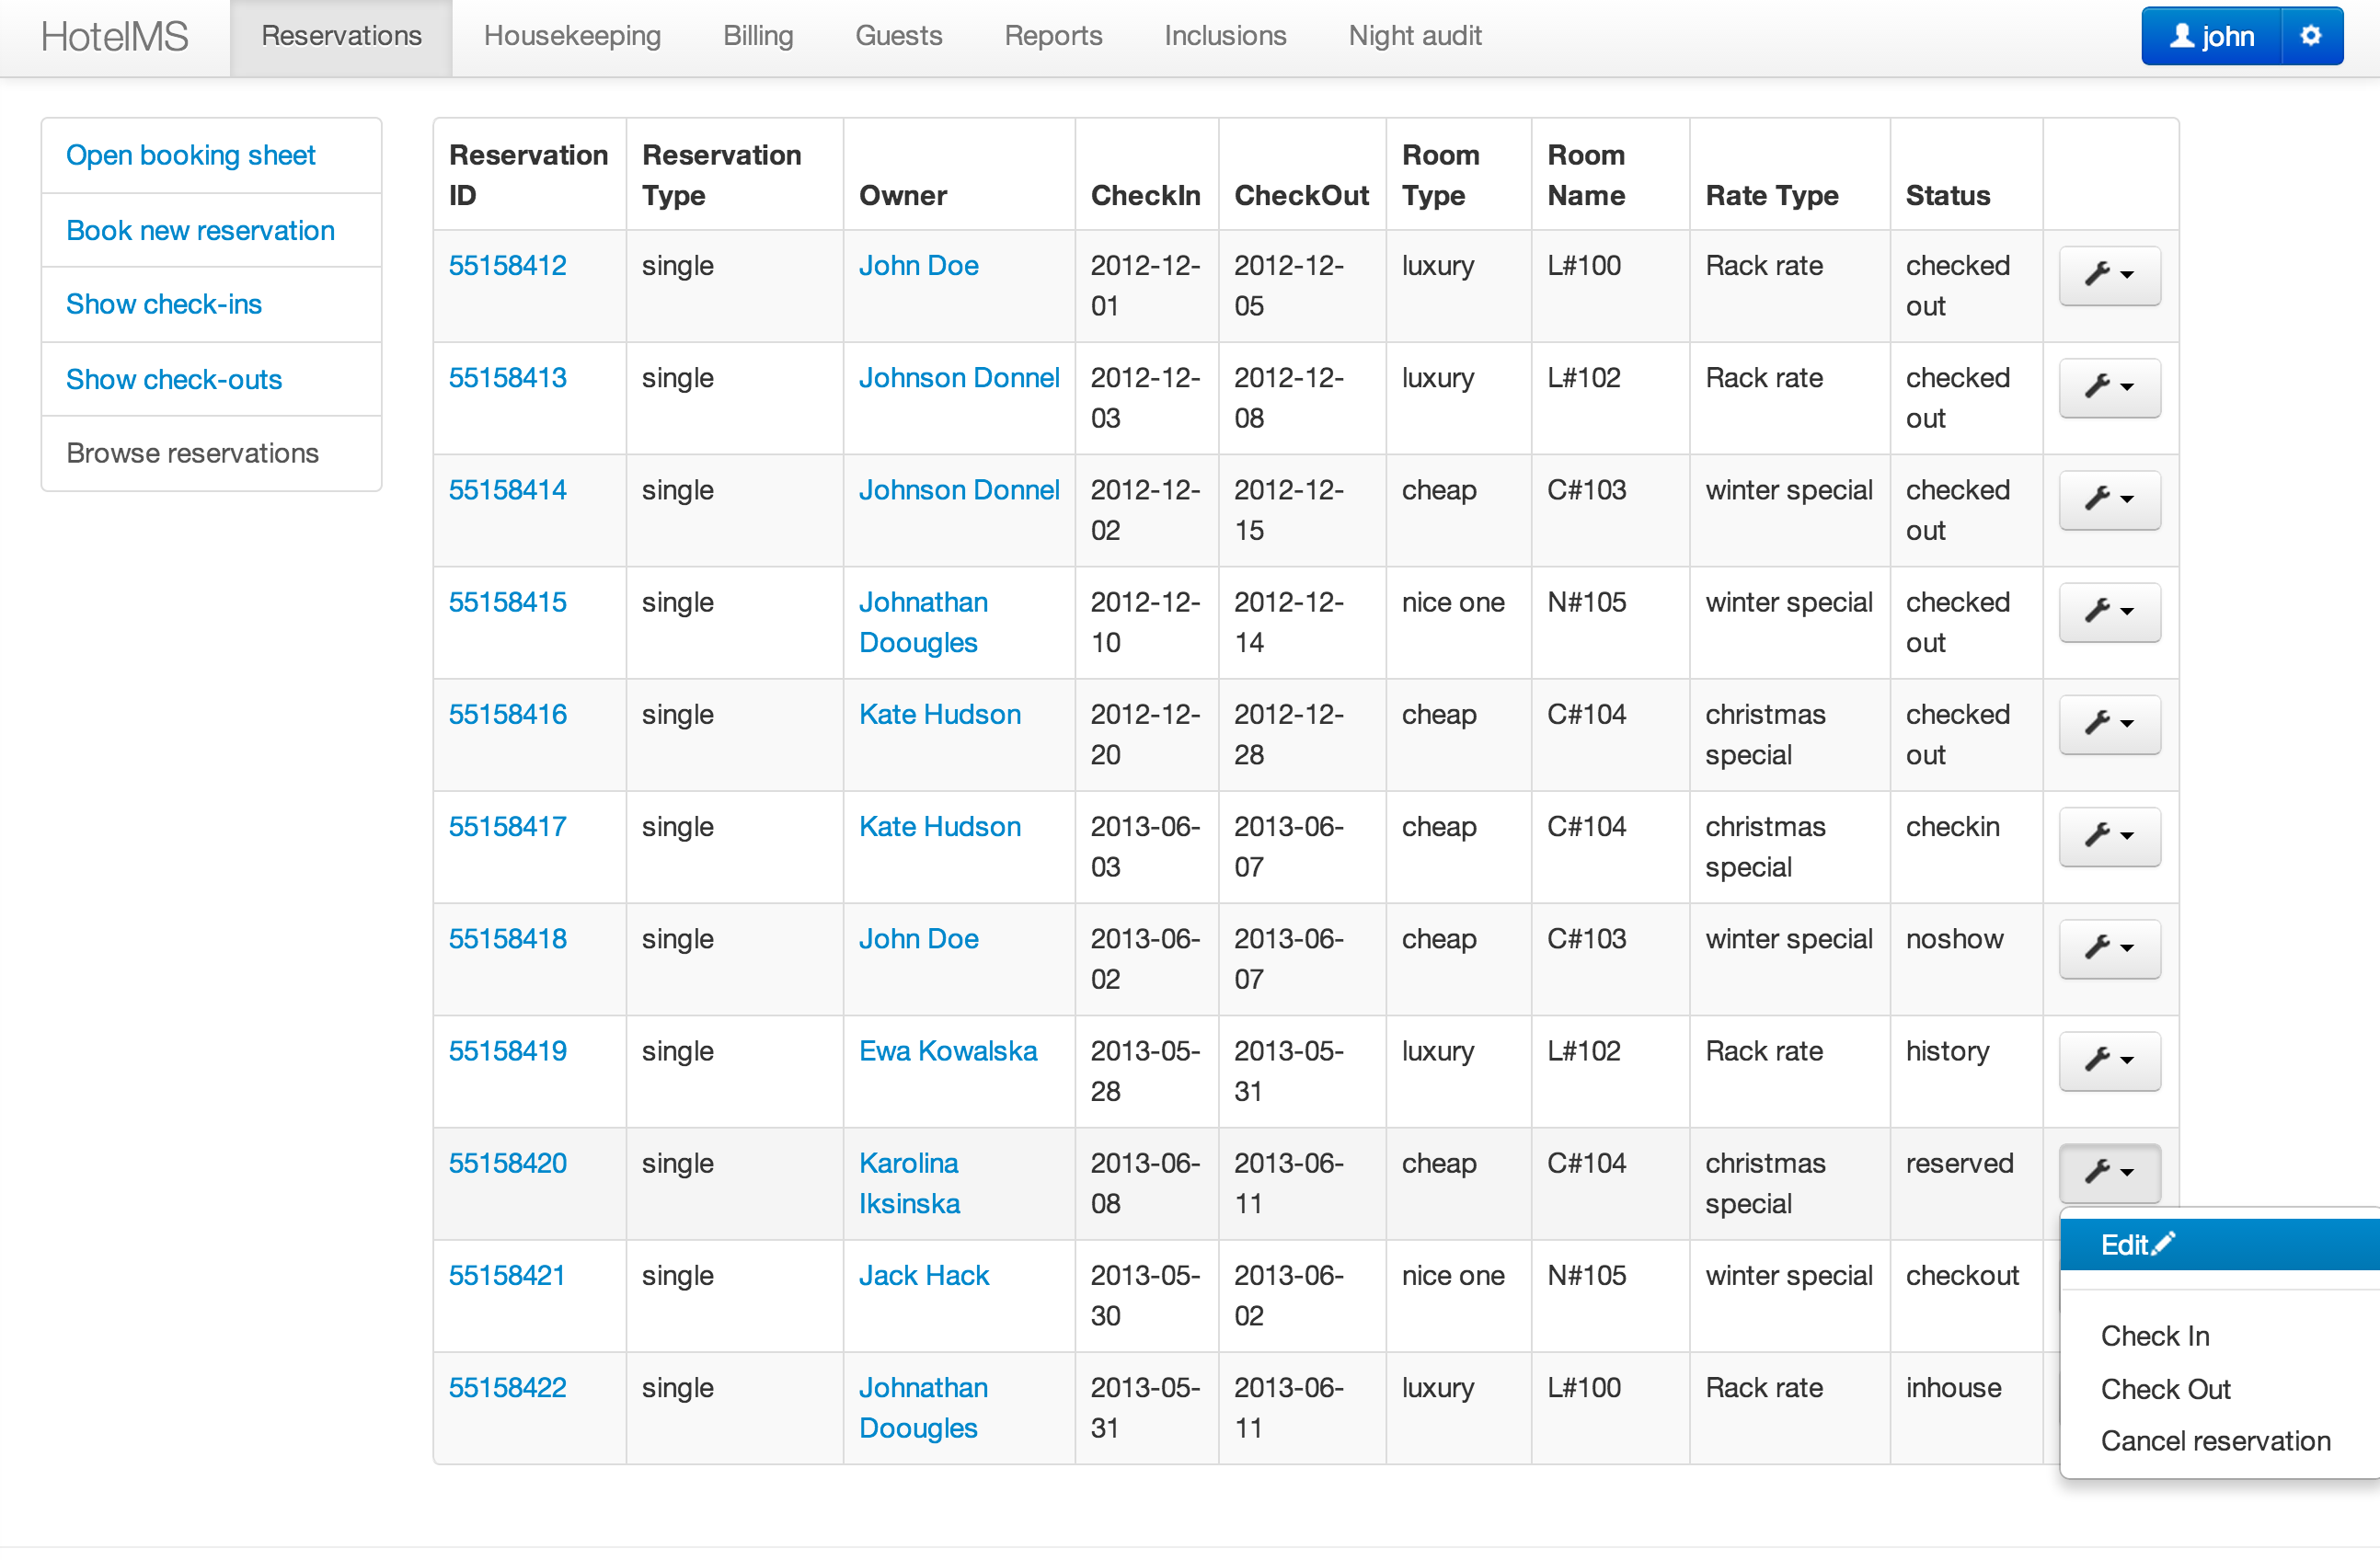
\includegraphics[scale=0.2, angle=270]{../img/wyglad/browse-reservations.png}
  }
  \end{center}
  \caption{Przegląd rezerwacji}
  \label{fig:app-browse-reservations}
\end{figure}

\begin{figure}[H]
  \begin{center}
  \fbox{
    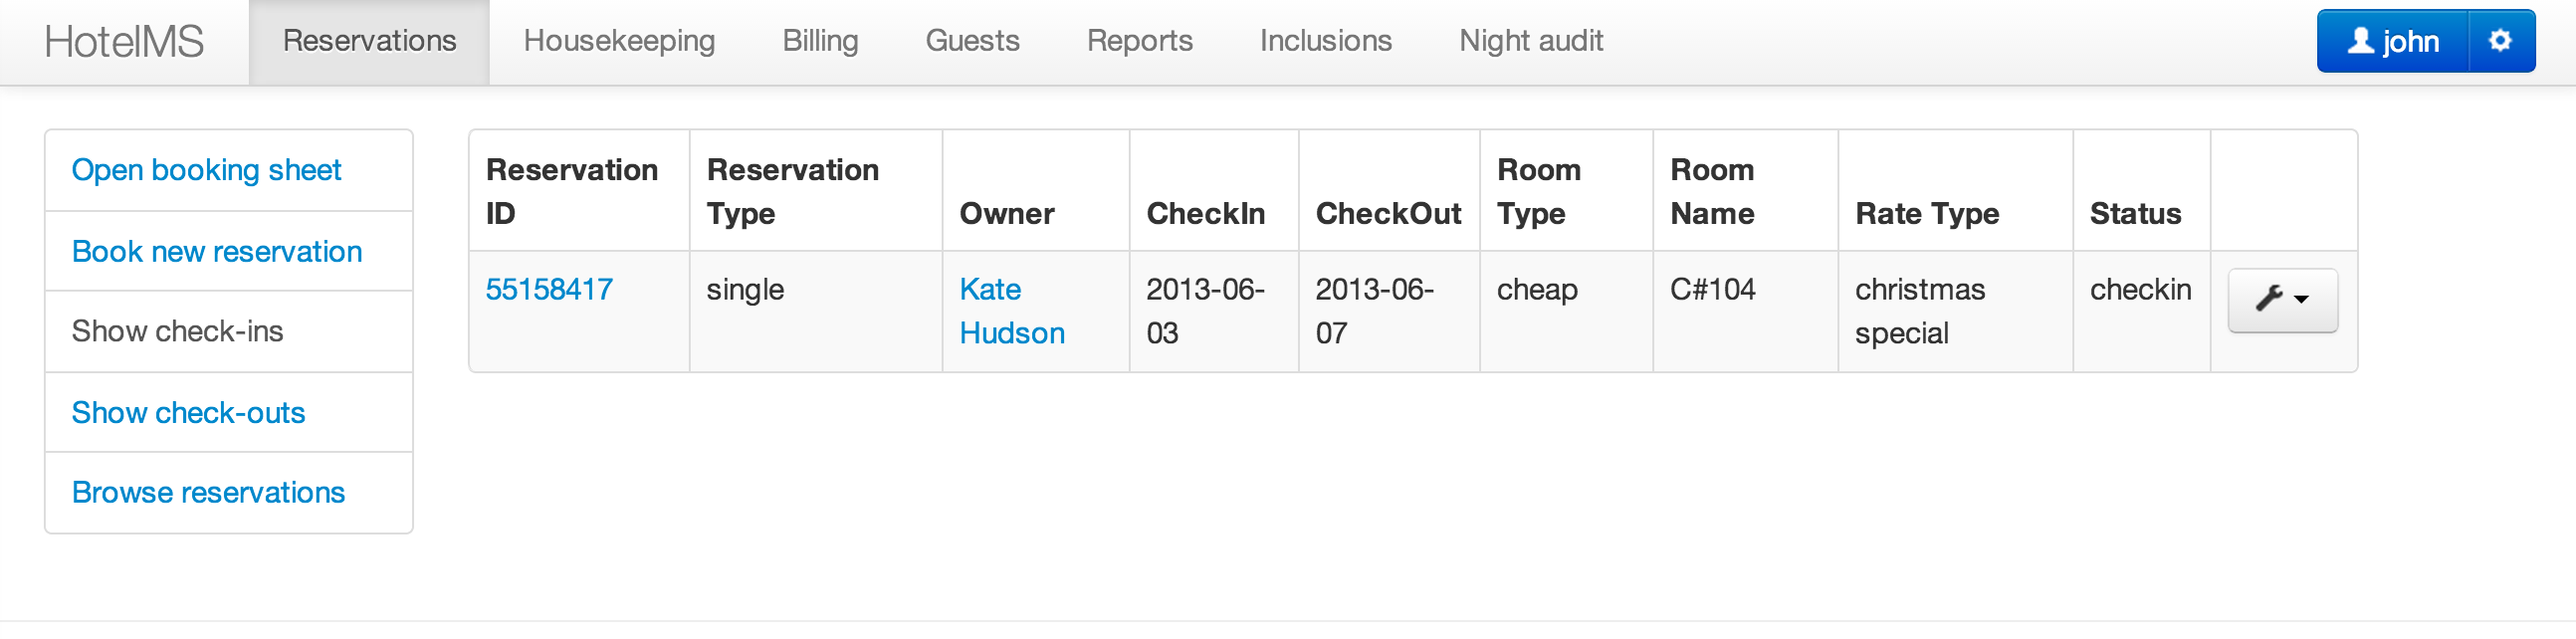
\includegraphics[scale=0.2, angle=270]{../img/wyglad/checkins.png}
  }
  \end{center}
  \caption{Lista przyjazdów}
  \label{fig:app-checkins}
\end{figure}

\begin{figure}[H]
  \begin{center}
  \fbox{
    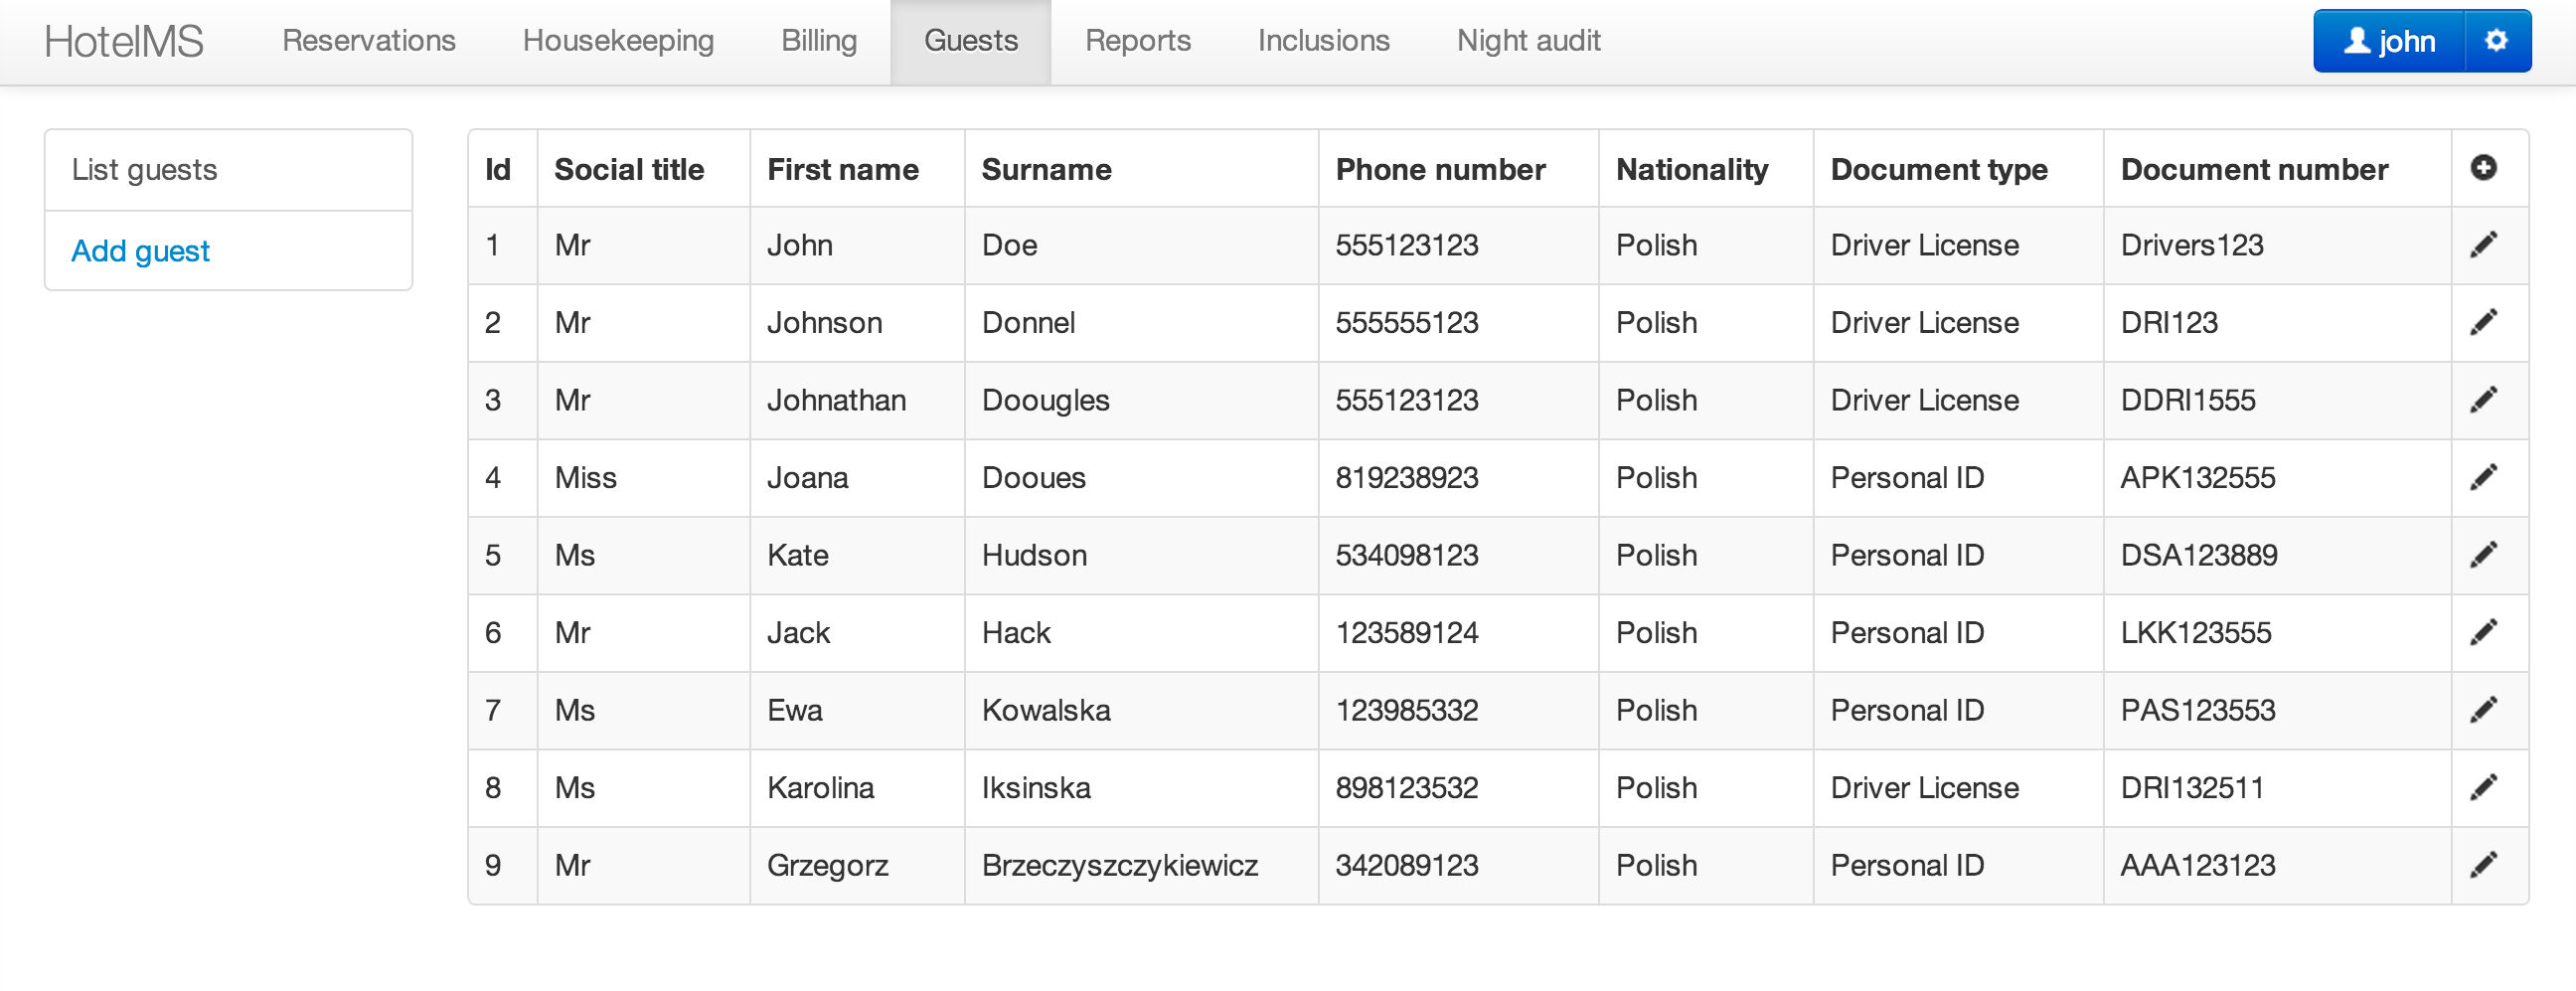
\includegraphics[scale=0.2, angle=270]{../img/wyglad/guest-list.png}
  }
  \end{center}
  \caption{Lista gości}
  \label{fig:app-guest-list}
\end{figure}

\begin{figure}[H]
  \begin{center}
  \fbox{
    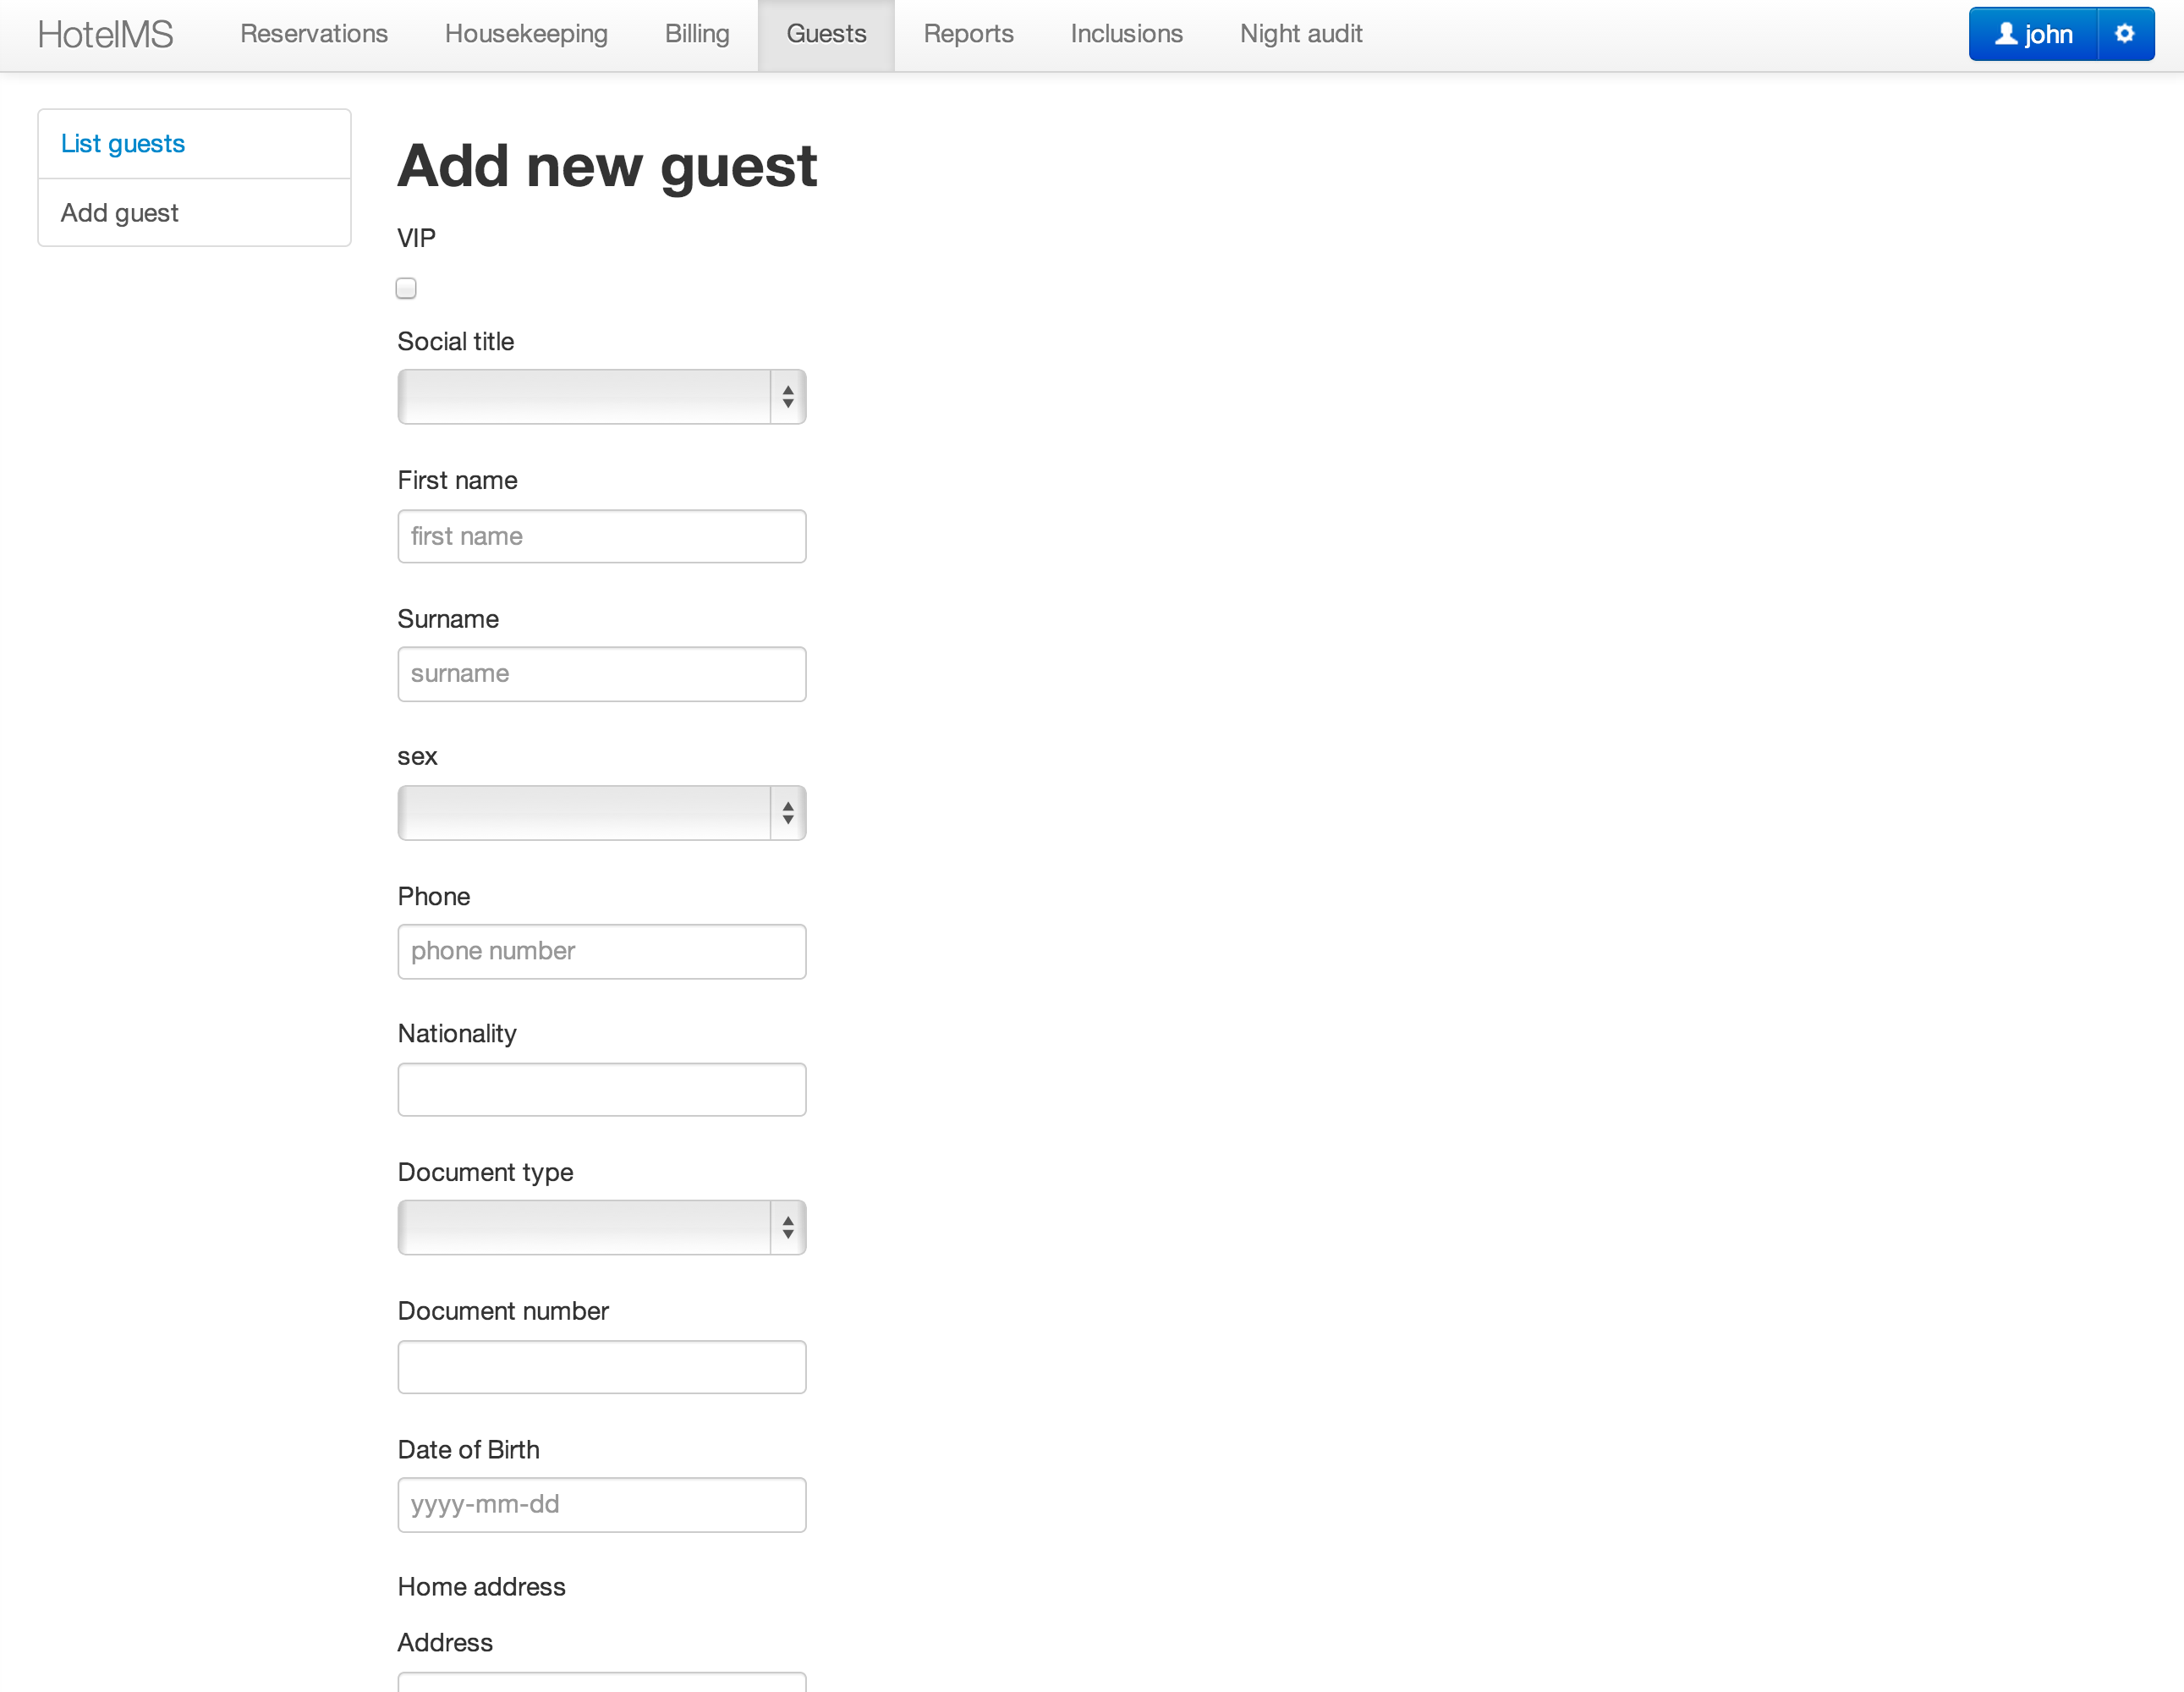
\includegraphics[scale=0.2, angle=270]{../img/wyglad/guest-form-part.png}
  }
  \end{center}
  \caption{Formularz nowego gościa}
  \label{fig:app-new-guest-form}
\end{figure}

\begin{figure}[H]
  \begin{center}
  \fbox{
    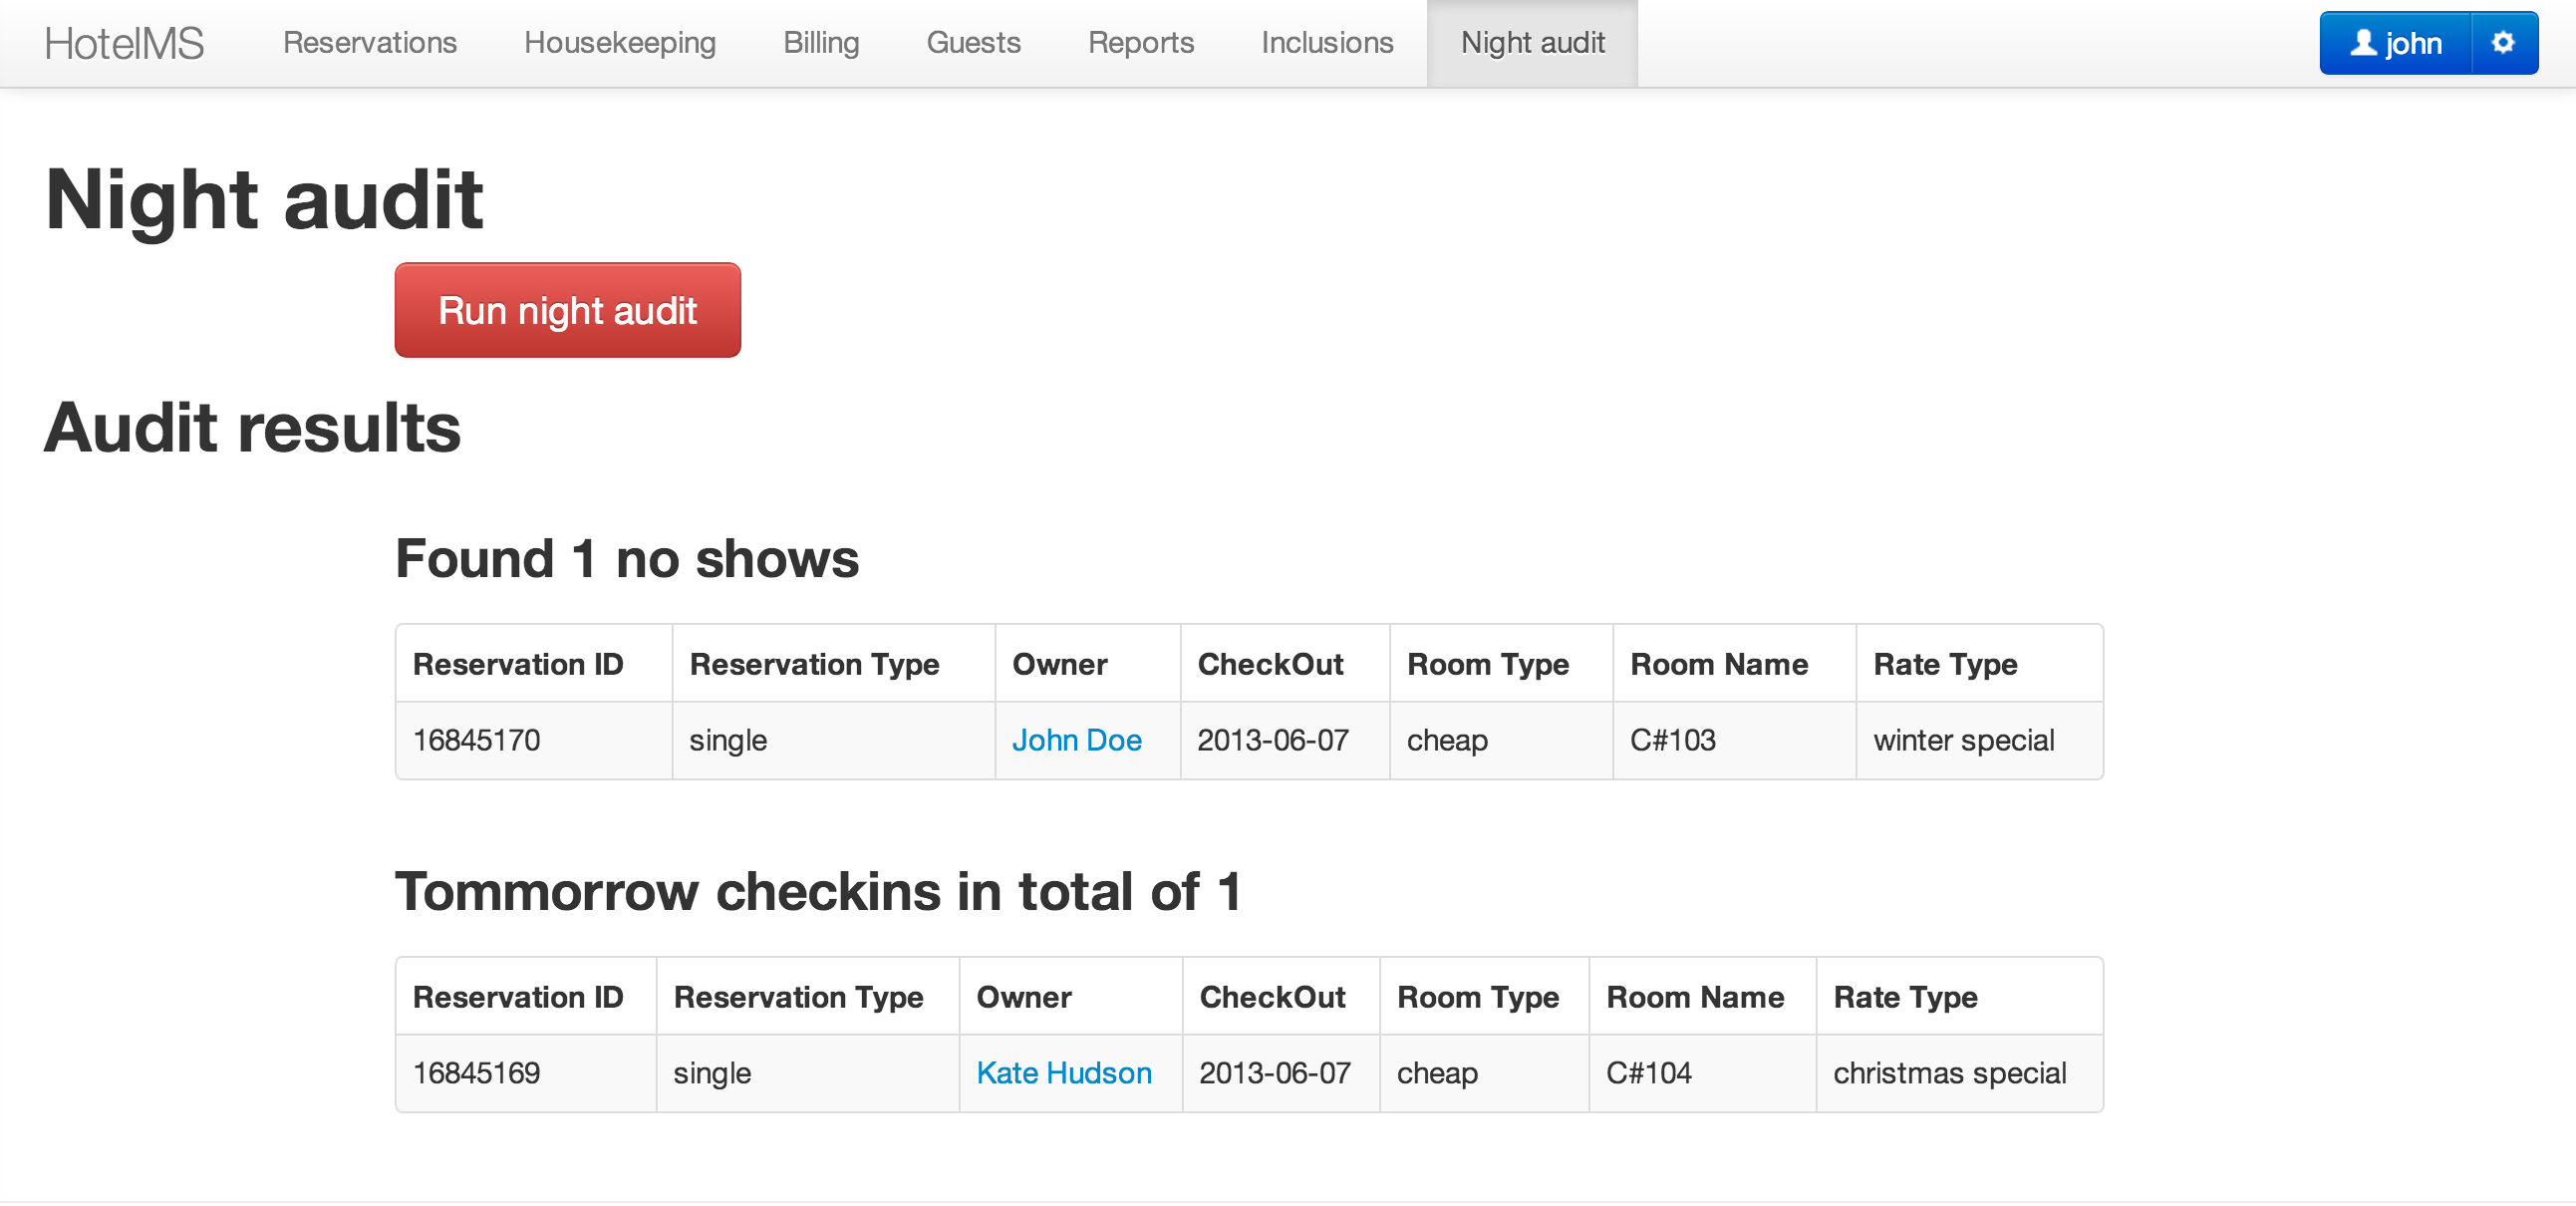
\includegraphics[scale=0.2, angle=270]{../img/wyglad/nightaudit.png}
  }
  \end{center}
  \caption{Wyniki nocnego audytu}
  \label{fig:app-nightaudit}
\end{figure}

% \begin{figure}[H]
%   \begin{center}
%   \fbox{
%     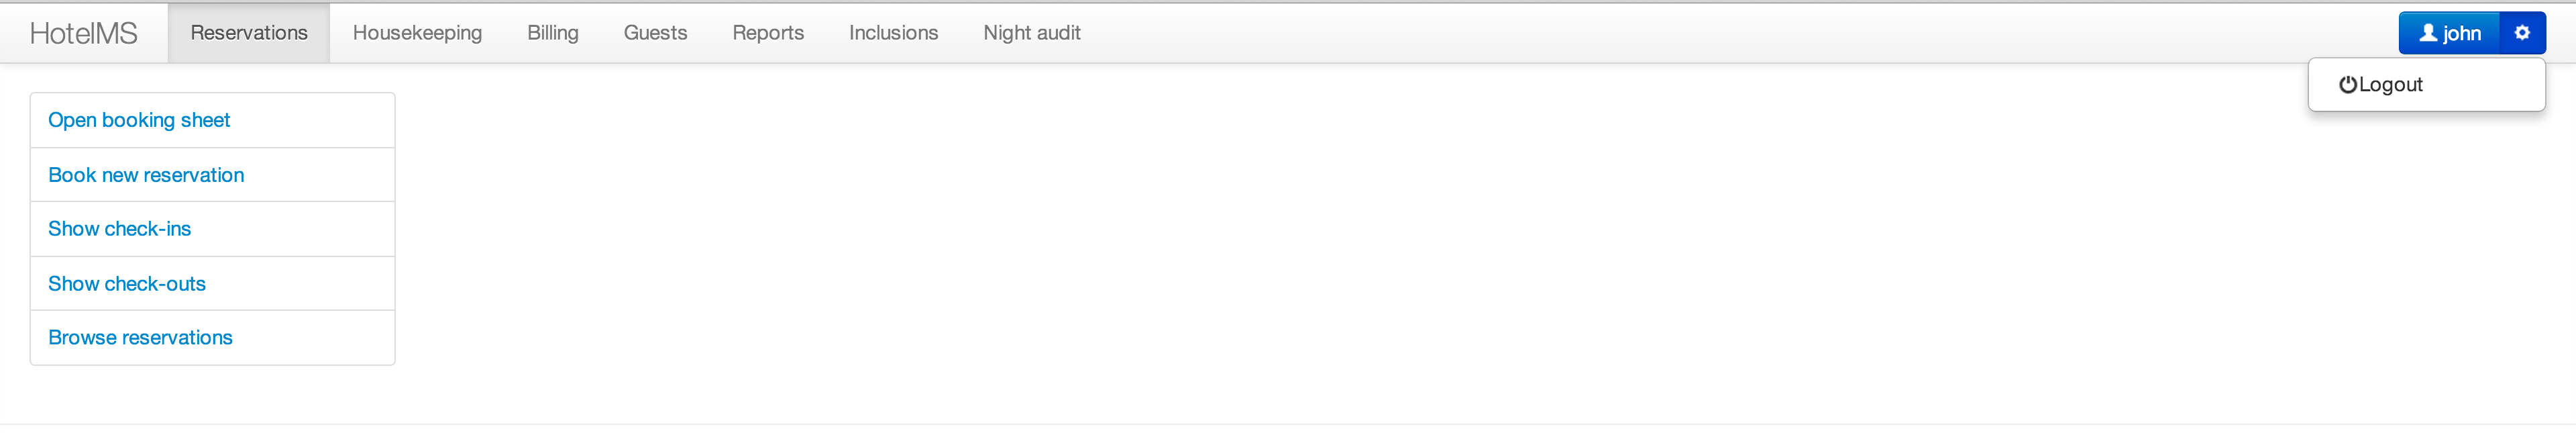
\includegraphics[scale=0.1, angle=270]{../img/wyglad/reservation-module-selected.png}
%   }
%   \end{center}
%   \caption{Główny ekran aplikacji z wybranym modułem rezerwacyjnym}
%   \label{fig:app-main}
% \end{figure}


% tutaj załączniki

%\chapter*{Bibliografia}
\nocite{*}
\bibliographystyle{plplain}
%\bibliographystylebk{plplain}
%\bibliographystylest{plplain}
%\bibliographystyledoc{plplain}
% \bibliographystyleweb{plplain}
%\bibliographybk{BIB/books}
%\bibliographyst{BIB/books}
%\bibliographydoc{BIB/books}
% \bibliographyweb{BIB/books}

% \bibliography{bib/verificard,bib/jml,bib/daikon}
\bibliography{../bib/daikon,../bib/statistics,../bib/other}

\end{document}

% ex: set tabstop=4 shiftwidth=4 softtabstop=4 noexpandtab fileformat=unix filetype=tex spelllang=pl,en spell:

